\documentclass[a4paper,11pt,twoside]{report}
\usepackage[english,polish]{babel}
\usepackage[utf8]{inputenc}
\usepackage[T1]{fontenc}
\usepackage[inner=3cm,outer=2cm,top=2.5cm,bottom=2.5cm]{geometry}
\usepackage{polski}
\usepackage{lipsum}
\usepackage{graphicx}
\usepackage{amsmath}   
\usepackage{nameref}
\usepackage{wrapfig}
\usepackage{hyperref}
\usepackage{gensymb}
\usepackage{textcomp}
\usepackage{float}
\usepackage{listings}
\usepackage{caption}
\usepackage{cleveref}
\usepackage{icomma}
\usepackage{dirtree}
\usepackage{fancyhdr}
\usepackage{minted}
\usepackage{siunitx}

%numercja stron
\fancypagestyle{plain}{%
\fancyhf{} % clear all header and footer fields
\fancyfoot[LE,RO]{\thepage}}
\renewcommand{\headrulewidth}{0pt}
\pagestyle{plain}

%czcionka bezszeryfowa
\renewcommand{\familydefault}{\sfdefault}


% Naprawa nazw z angielskiego
\def\figureautorefname{Rysunek}

%Strona streszczenia
\newenvironment{abstractpage}
  {\cleardoublepage\vspace*{\fill}\thispagestyle{empty}}
  {\vfill\cleardoublepage}
  
%Samo streszczenie
\newenvironment{abstractsection}[1]
  {\bigskip\selectlanguage{#1}%
   \begin{center}\bfseries\abstractname\end{center}}
  {\par\bigskip}

%Ładne ułamki w jednostkach fizycznych
\sisetup{per-mode=symbol}%


\begin{document}
\begin{titlepage}
\pagestyle{empty}

\noindent
\begin{large}
\begin{table}[t]
\centering
\begin{tabular}[t]{lcr}
 
\includegraphics[width=70pt,height=70pt]{graphics/pw_logo.jpg} & Politechnika Warszawska & 
\includegraphics[width=70pt,height=70pt]{graphics/weiti_logo.pdf}\\
& Wydział Elektroniki i & \\
& Technik Informacyjnych &
\end{tabular}
\end{table}

\begin{center}Sprawozdanie z Pracowni Dyplomowej \\ Inżynierskiej I --- PDI2\end{center}
\begin{center}Informatyka\end{center}\end{large}

\vfill
\begin{center}
\large
Tytuł: \\
\Huge
Symulacja dookólnej bazy mobilnej
\end{center}

\vfill
\begin{center}
\large
Autor: \\
\Large
Radosław Świątkiewicz
\end{center}

\vfill
\begin{center}
\large
Opiekun naukowy: \\
\Large
dr hab. inż. Wojciech Szynkiewicz
\end{center}

\vfill
\begin{center}
Warszawa, \today
\end{center}

\end{titlepage}
\begin{abstract}
Ta praca opisuje projektowanie i budowę środowiska symulacyjnego dla wielokierunkowej platformy mobilnej, poruszającej się za pomocą kół szwedzkich.

Platforma jest bazą mobilną dla dwuramiennego robota Velma. 
Celem pracy jest stworzenie możliwie dokładnego modelu symulacyjnego rzeczywistej bazy mobilnej.
Model ten ma służyć do wstępnych badań algorytmów planowania ruchu i sterowania robotem mobilnym.

Rozpatrzone są tutaj wymagania i problemy przy tworzeniu każdego ze składników środowiska.
Na system składają się wirtualne efektory i receptory obsługujące odpowiednią maszynę symulacyjną, a także komponenty wspomagające symulację.
\end{abstract}
 


\tableofcontents

\chapter{Wstęp}
\section{Cel}
Celem tej pracy inżynierskiej jest budowa środowiska robota mobilnego w przestrzeni wirtualnej.
Za zadanie jest stworzyć oprogramowanie modelu 3D, oraz modelu dynamiki wielokierunkowej platformy mobilnej z kołami szwedzkimi. 
Wymaga się, aby model i obsługujące go oprogramowanie było dokładną kopią prawdziwego robota, dzięki czemu zachowanie symulacji będzie jak najbardziej zbliżone do zachowania fizycznego obiektu.
Opisywana platforma będzie używana jako baza wielokierunkowa do przemieszczania dwuramiennego robota manipulującego Velma.

Należy tak opisać model, aby reagował na siły podobnie do rzeczywistej wersji i przyjmował to samo sterowanie z zewnątrz, co rzeczywisty obiekt.
To spowoduje, że możliwe będzie stworzenie jednego wspólnego programu sterującego do użycia zarówno w wirtualnej wersji, jak i fizycznej.

Testowanie oprogramowania na prawdziwym obiekcie może prowadzić do jego uszkodzeń, dlatego wpierw trzeba się upewnić o poprawności projektowanych rozwiązań na bezpiecznej kopii wirtualnej.
Rzeczywistość nie pozwala także na przeprowadzanie zaawansowanych scenariuszy środowiska testowego.
Szybciej i taniej jest stworzyć wirtualne środowisko testowe, niż fizyczne, w dodatku porażka sterowników przy symulacji nie wpływa na zniszczenie robota w rzeczywistości.
Dopiero przy osiągnięciu satysfakcjonującej jakości sterowania w symulacji wirtualnej można zastosować algorytmy sterowania do oryginalnego obiektu bez ryzyka uszkodzeń urządzenia.

Należy także móc obsługiwać czujniki, za pomocą których oprogramowanie orientuje się w przestrzeni i generuje sterowanie.
Wirtualizacja czujników polega na generowaniu danych na podstawie symulacji.
W celu przybliżenia wyjścia takiego programu do rzeczywistego urządzenia, do generowanych danych zwykle dodaje się szum, oraz błędy.
%%%
\section{Wielokierunkowa platforma mobilna}
\begin{figure}
\centering
 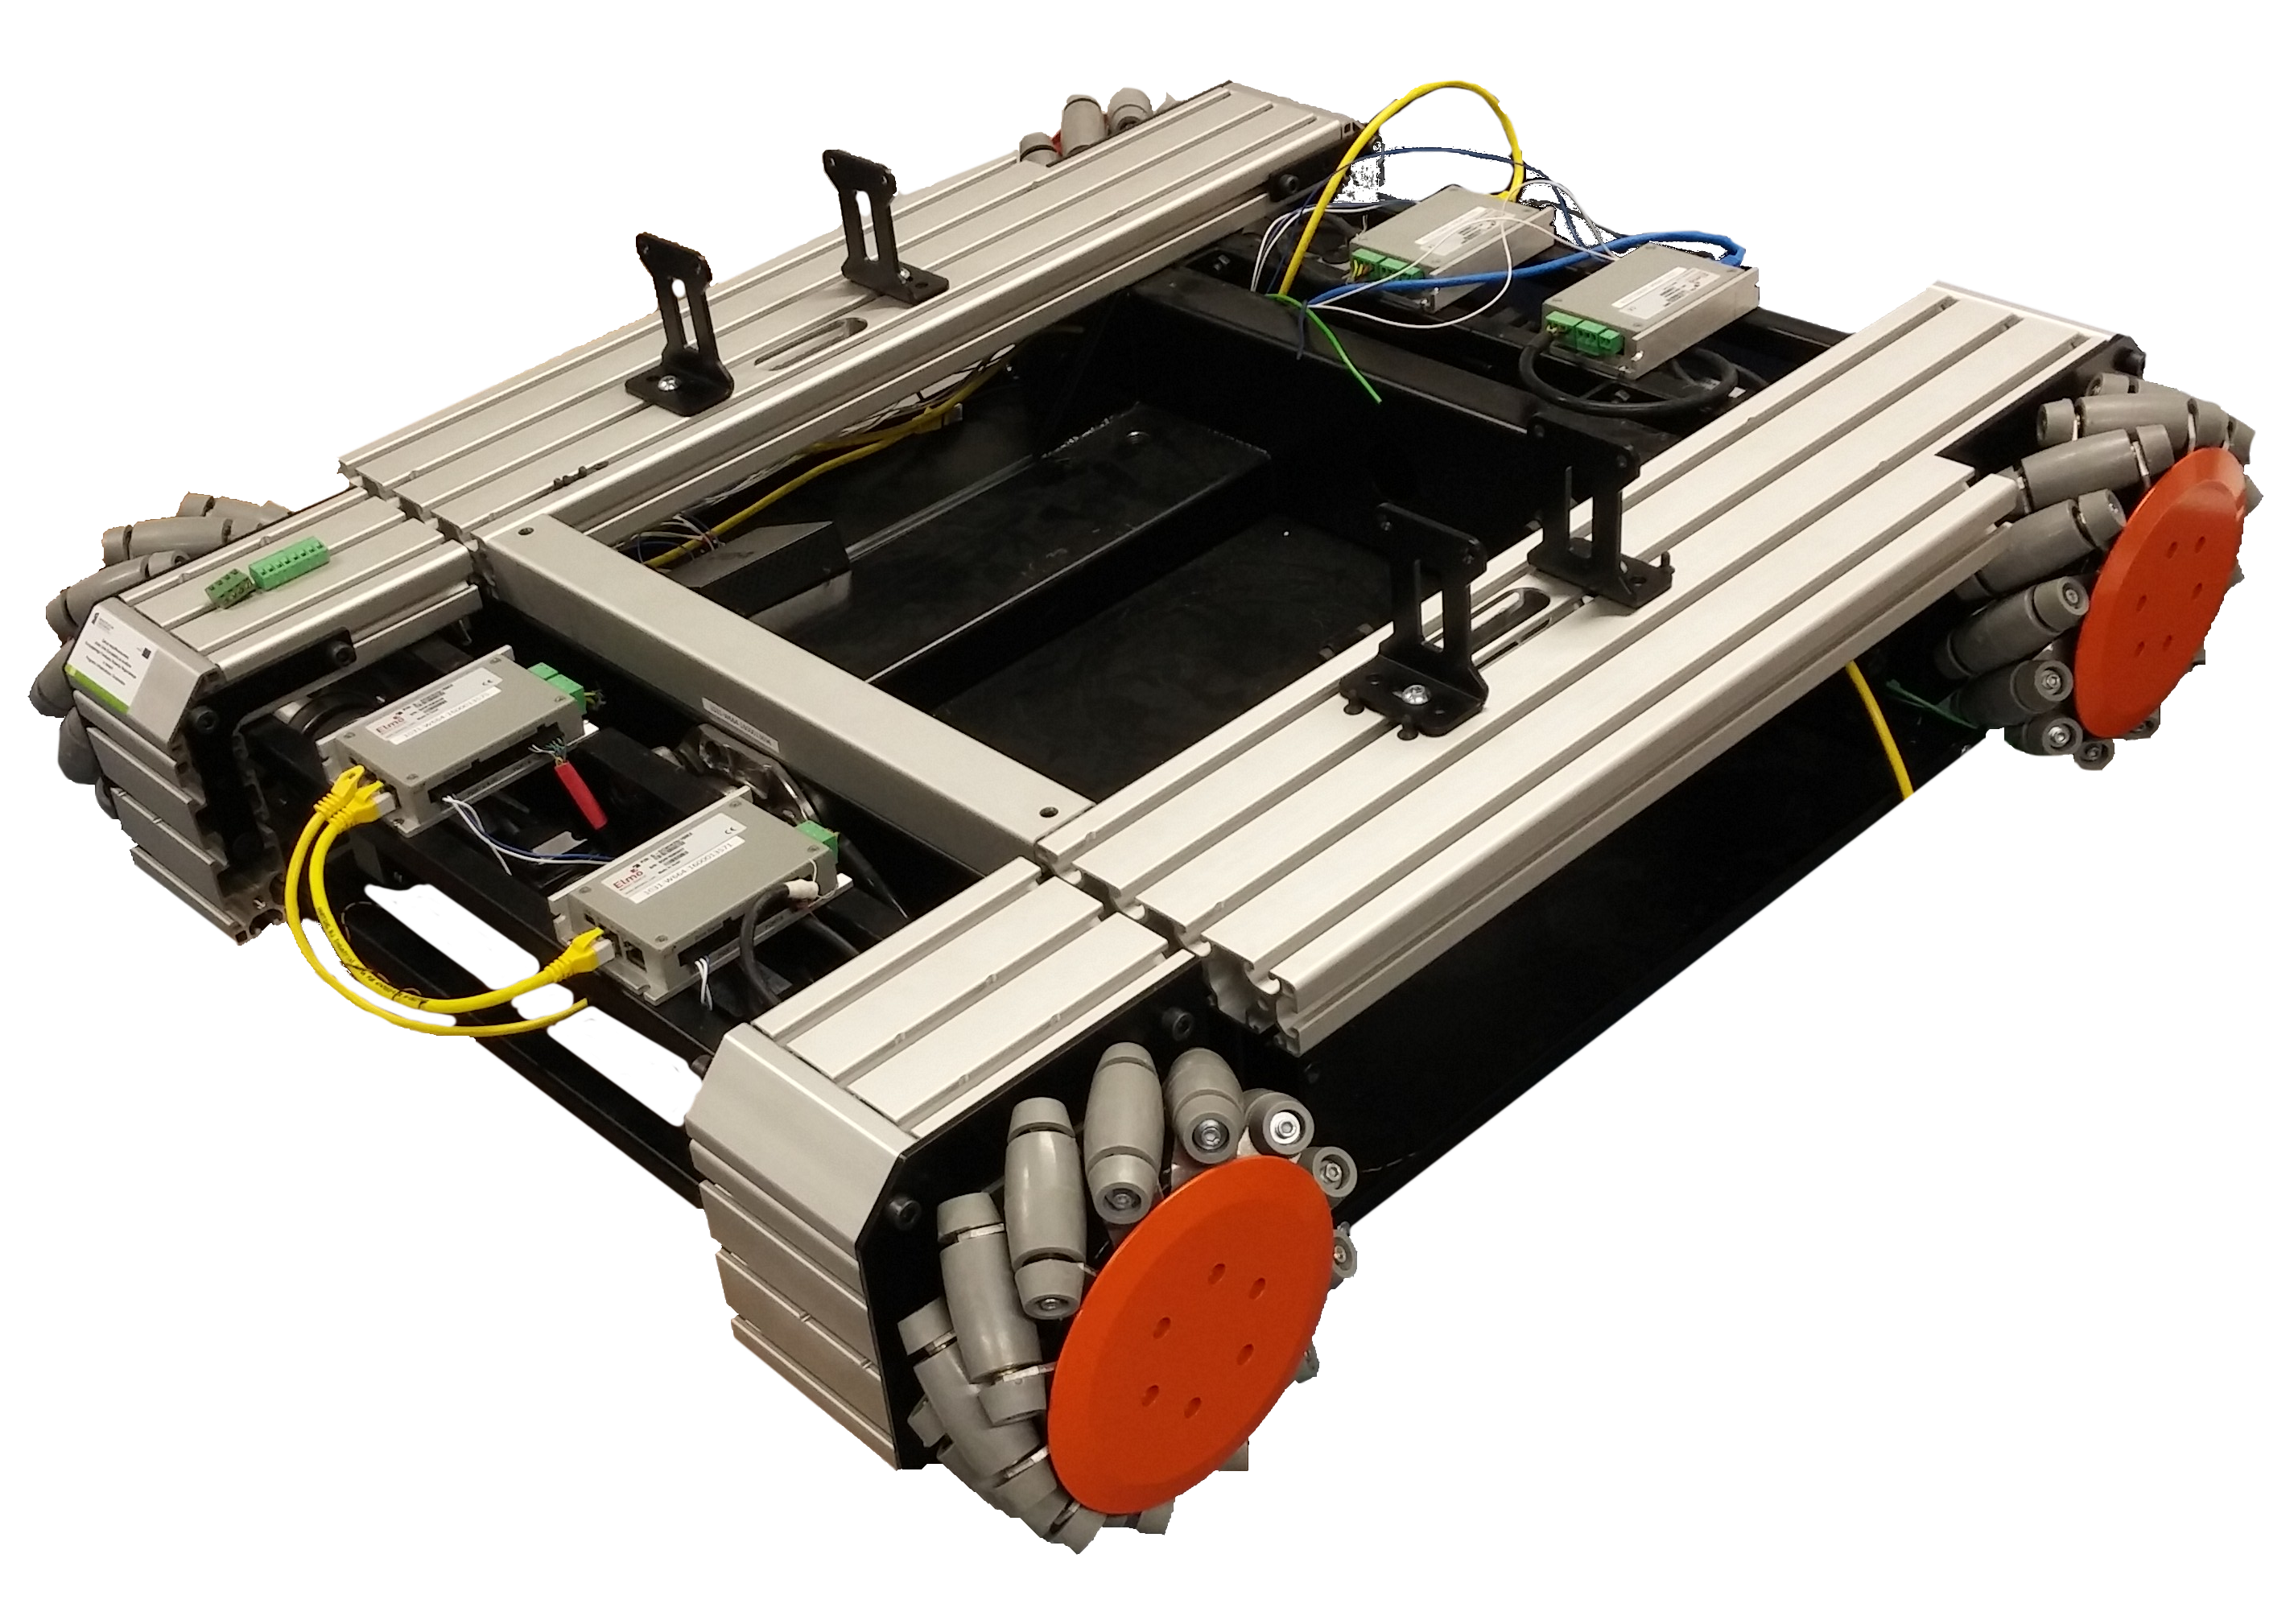
\includegraphics[width=0.8\textwidth]{graphics/base_photo.png}
\caption{Fotografia platformy z perspektywy. Niebieskie urządzenia na szczycie to czujniki laserowe.}
\end{figure} 
Jest to duża, prostokątna podstawa dookólna jeżdżąca na czterech kołach szwedzkich.
Koła są stałe, parami przyczepione do dwóch osi.
Każde koło jest sterowane osobno przez serwomotor, może mieć prędkość i kierunek niezależny od reszty kół i kierunku poruszania się robota.
Każdy z serwomotorów ma także wbudowany enkoder do sprawdzania rzeczywistego kąta obrotu.

Koła szwedzkie, zwane także kołami Mecanum, to specjalne koła z dodatkowymi rolkami na obwodzie ustawionymi pod kątem $45^\circ$ do osi koła.
Rolki nie mają silników i obracają się niezależnie od siebie.
Ich osie ustawione są tak, że osie rolek dwóch kół z tej samej strony robota są pod kątem prostym i przecinają się pośrodku urządzenia.
Innymi słowy, robot ma identycznie ustawione koła na przeciwległych wierzchołkach, i razem ustawione są w kształt litery \emph{X}.

Odpowiedni obrót kół względem siebie pozwala na ruch platformy w dowolnym kierunku niezależnie od kąta obrotu robota.
Za ich pomocą da się także obracać całością w czasie jazdy.
Jeśli na przykład obracać tylko przeciwległymi kołami po przekątnej, system zacznie się poruszać po skosie.
A jeśli do tego dodamy obrót kół drugiej przekątnej w odwrotnym kierunku, wtedy pojazd pojedzie w bok pomimo faktu, że koła nie zmieniły swojej osi i się nie przekręciły.

Podstawa ma za zadanie wozić wydziałowego robota manipulującego Velma.
Jest to wysoki i bardzo ciężki robot wyposażony w dwa chwytaki na ramionach o licznych przegubach.
Konstrukcja powoduje, że sama podstawa potrzebuje mieć sporą nośność i szerokość, aby zachować środek ciężkości bezpiecznie nisko.
Jeżdżąc na tej podstawie robot może się przemieszczać i obracać w dowolnym kierunku, aby uzyskać lepszy dostęp do manipulowanych przedmiotów.

Z jednej strony platformy znajduje się zawias oddzielający główną część od drugiej nieco mniejszej.
Części łączy wspólna oś, wygląda to tak, jakby przeciąć podstawę w poprzek i połączyć obie części przegubem na środku.

Ma to za zadanie zapewnić, aby każde koło dociskało do podłoża z taką samą siłą, jak to po drugiej stronie osi.
Pozwala to także na pokonywanie drobnych nierówności terenu.
Bez tego zawiasu nierówna podłoga spowodowała by, że na przykład tylko trzy koła dotykałyby podłoża w danym momencie uniemożliwiając sprawne sterowanie.
Niedeterministyczne tarcie kół jest niewykrywalne w bezpośredni sposób, więc należy je wyeliminować w jeden z tych sposobów.

\begin{figure}
\centering
 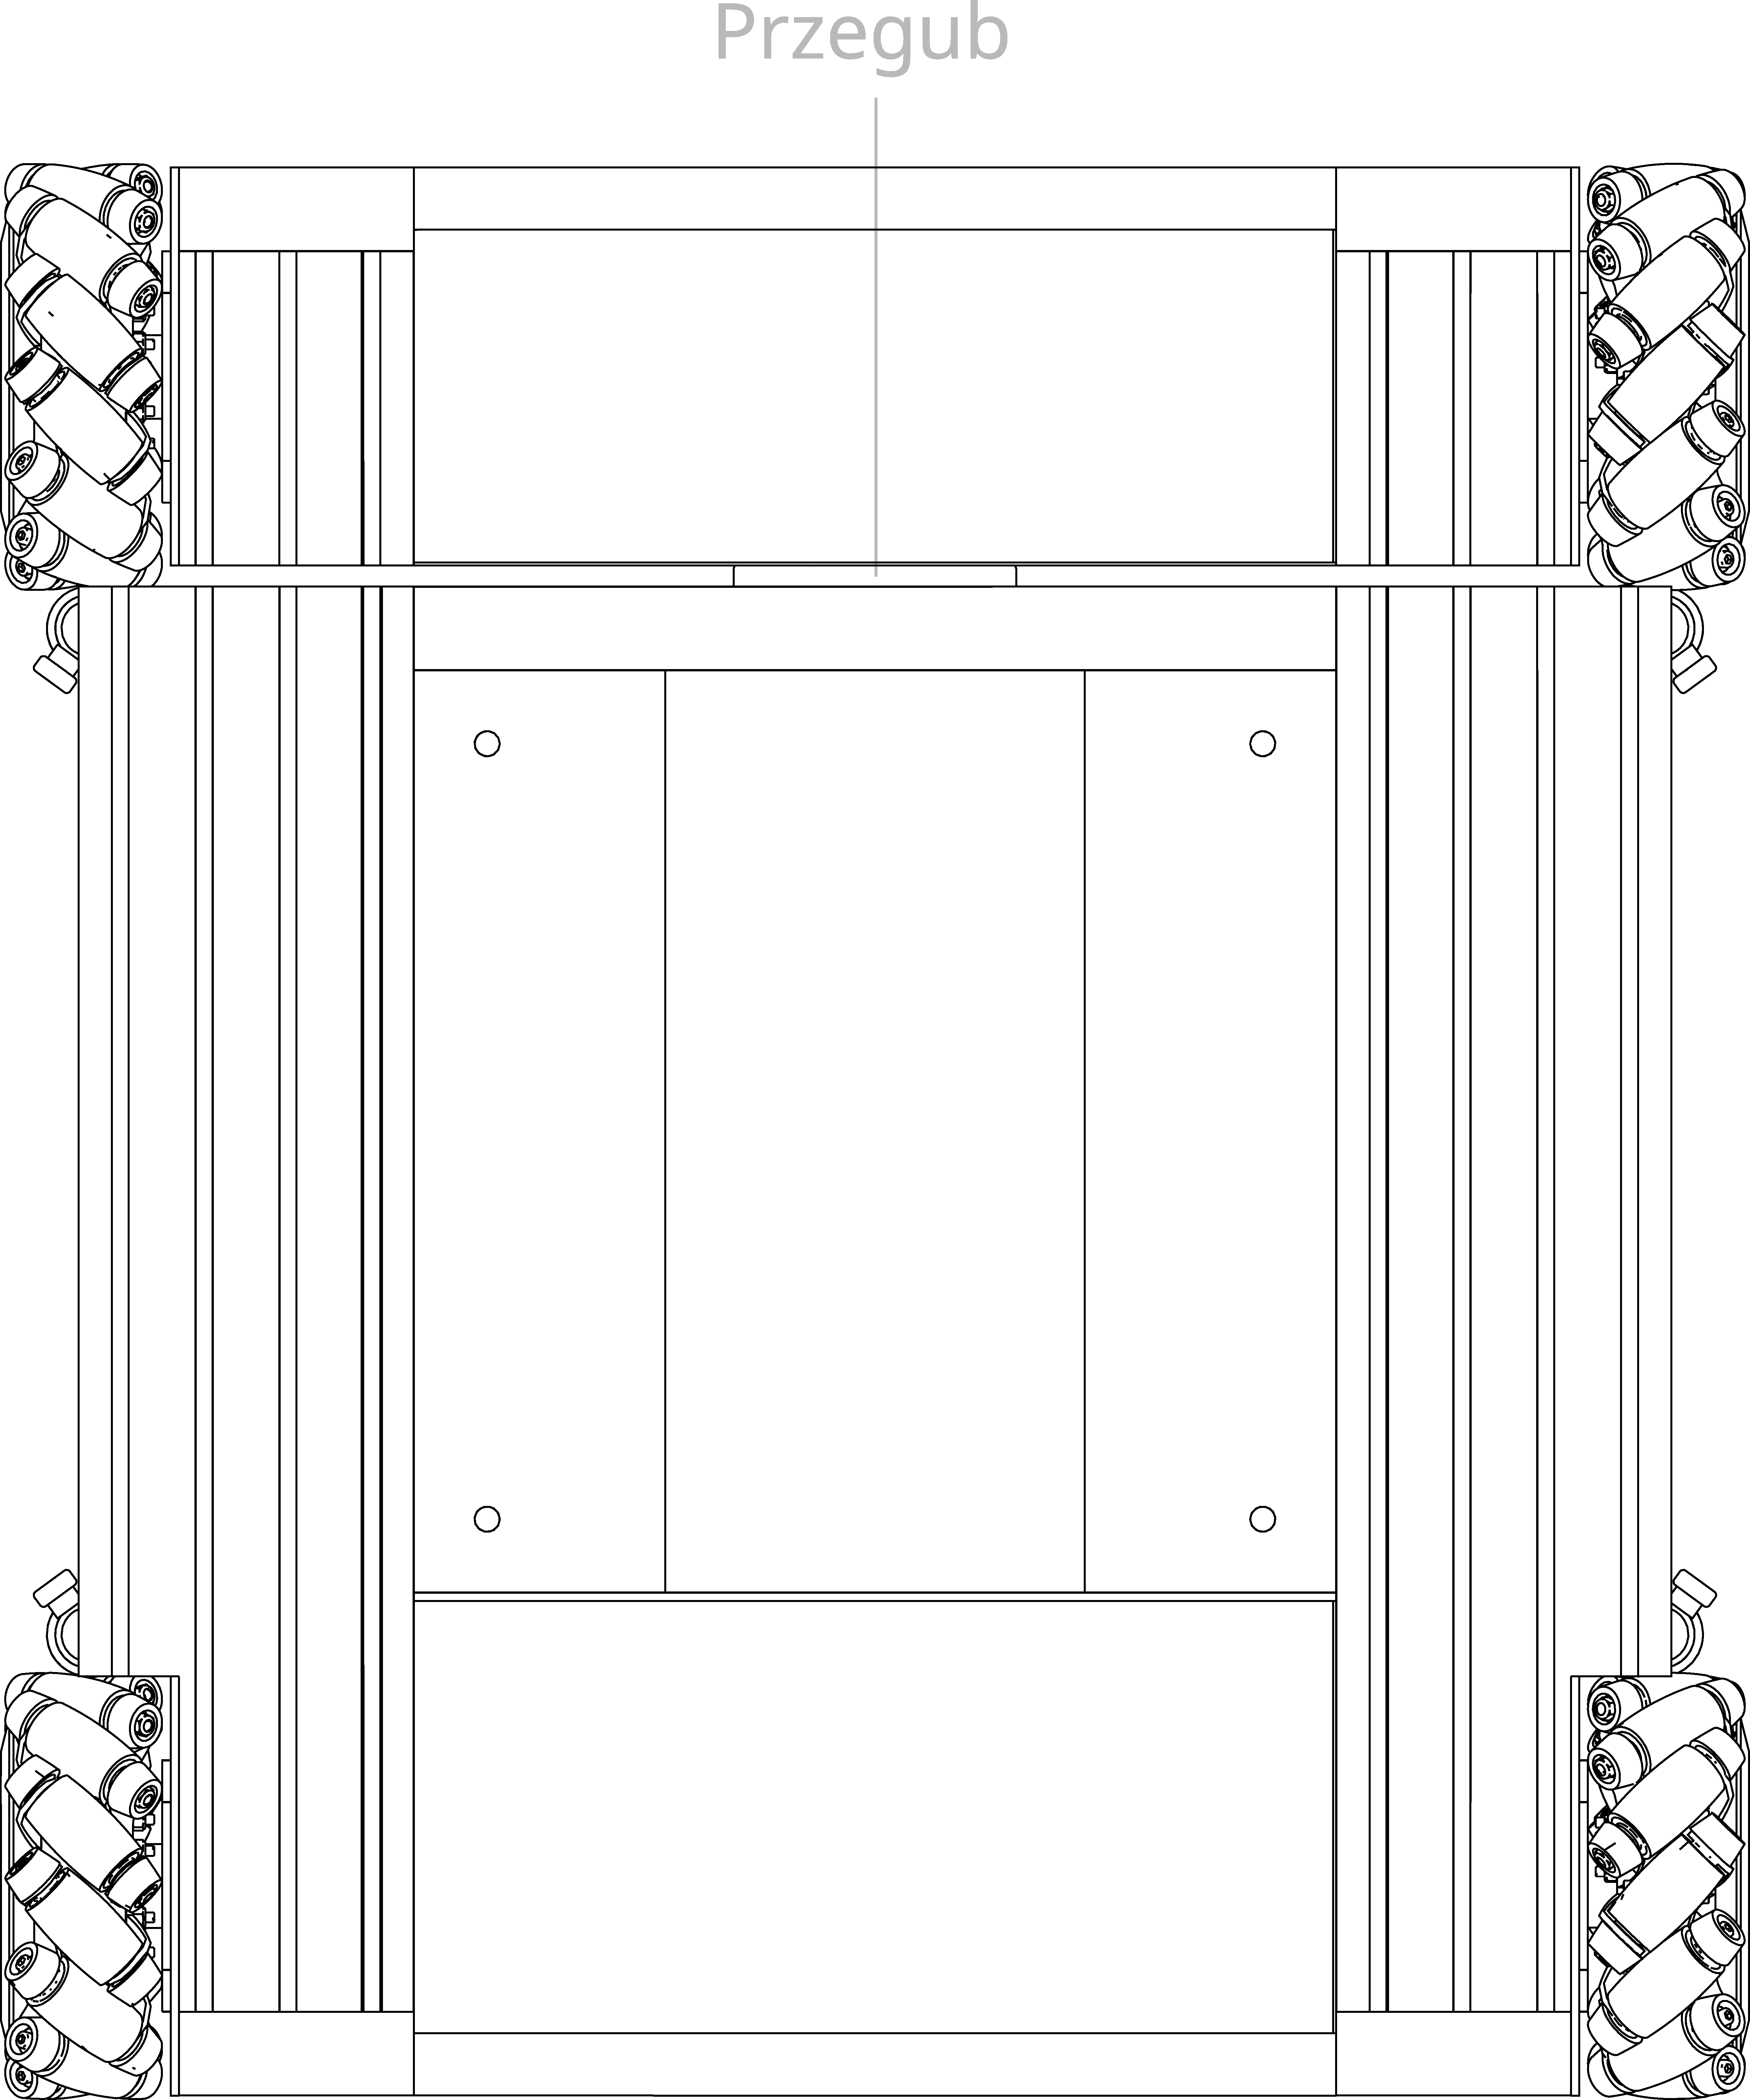
\includegraphics[width=0.5\textwidth]{graphics/base_top.pdf}
\caption{Platforma mobilna widziana od góry.}
\end{figure} 

\begin{figure}
\centering
 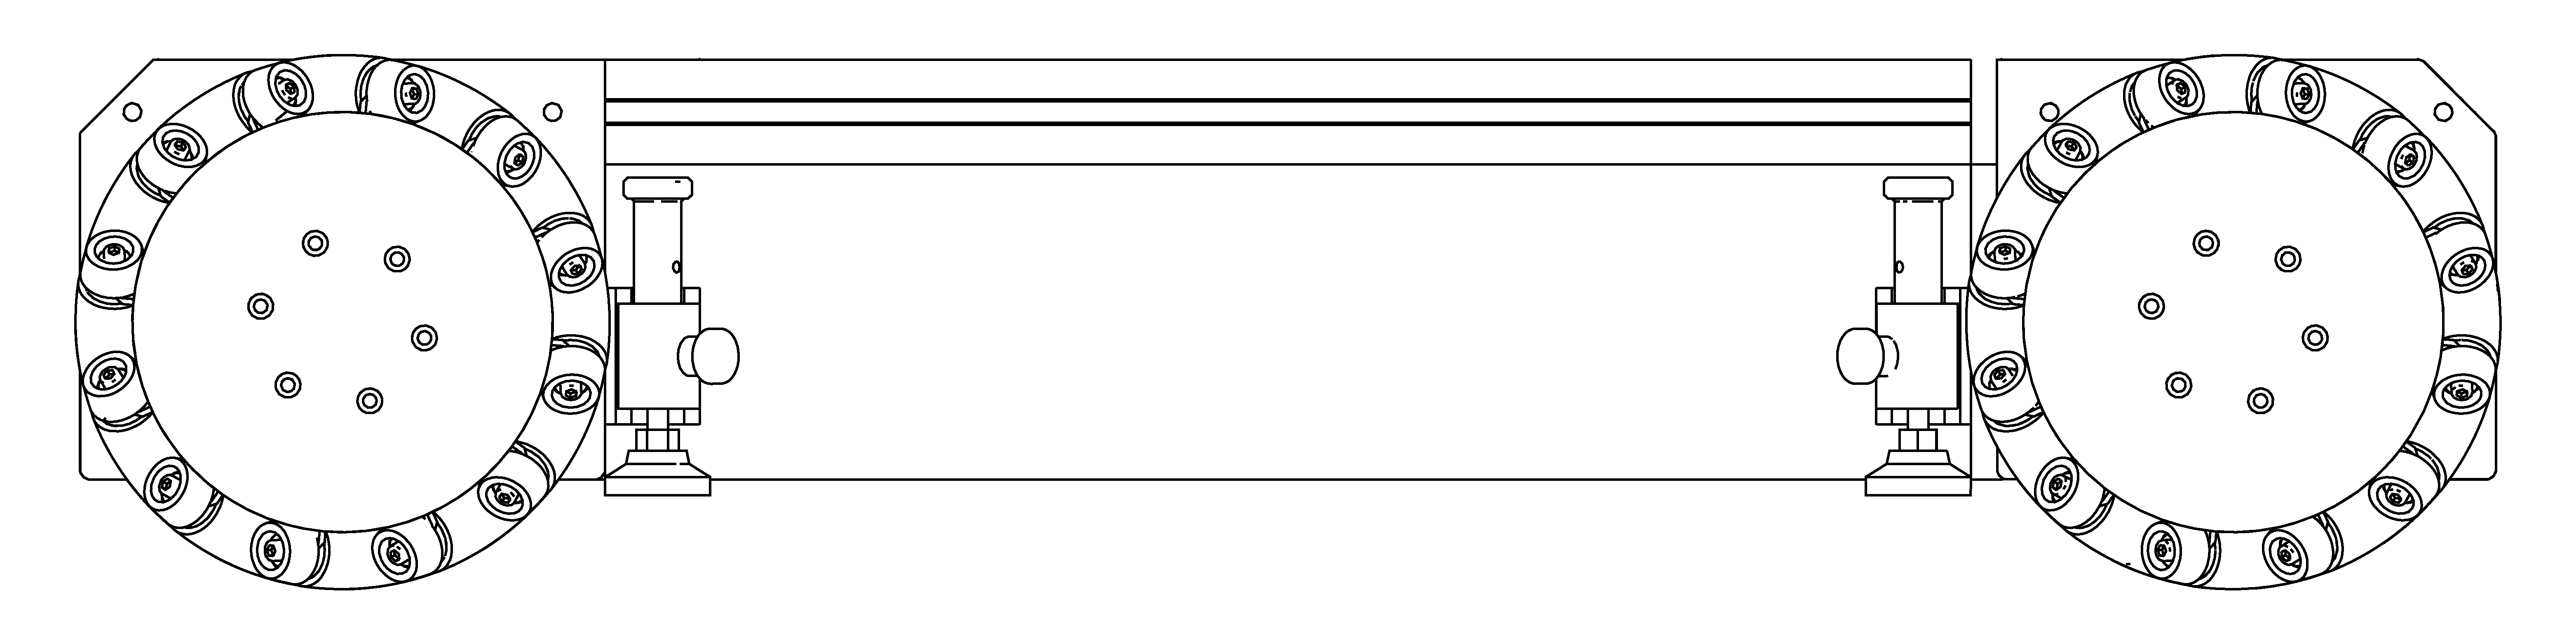
\includegraphics[width=0.5\textwidth]{graphics/base_side.pdf}
\caption{Platforma mobilna widziana od prawej strony.}
\end{figure} 

\begin{figure}
\centering
 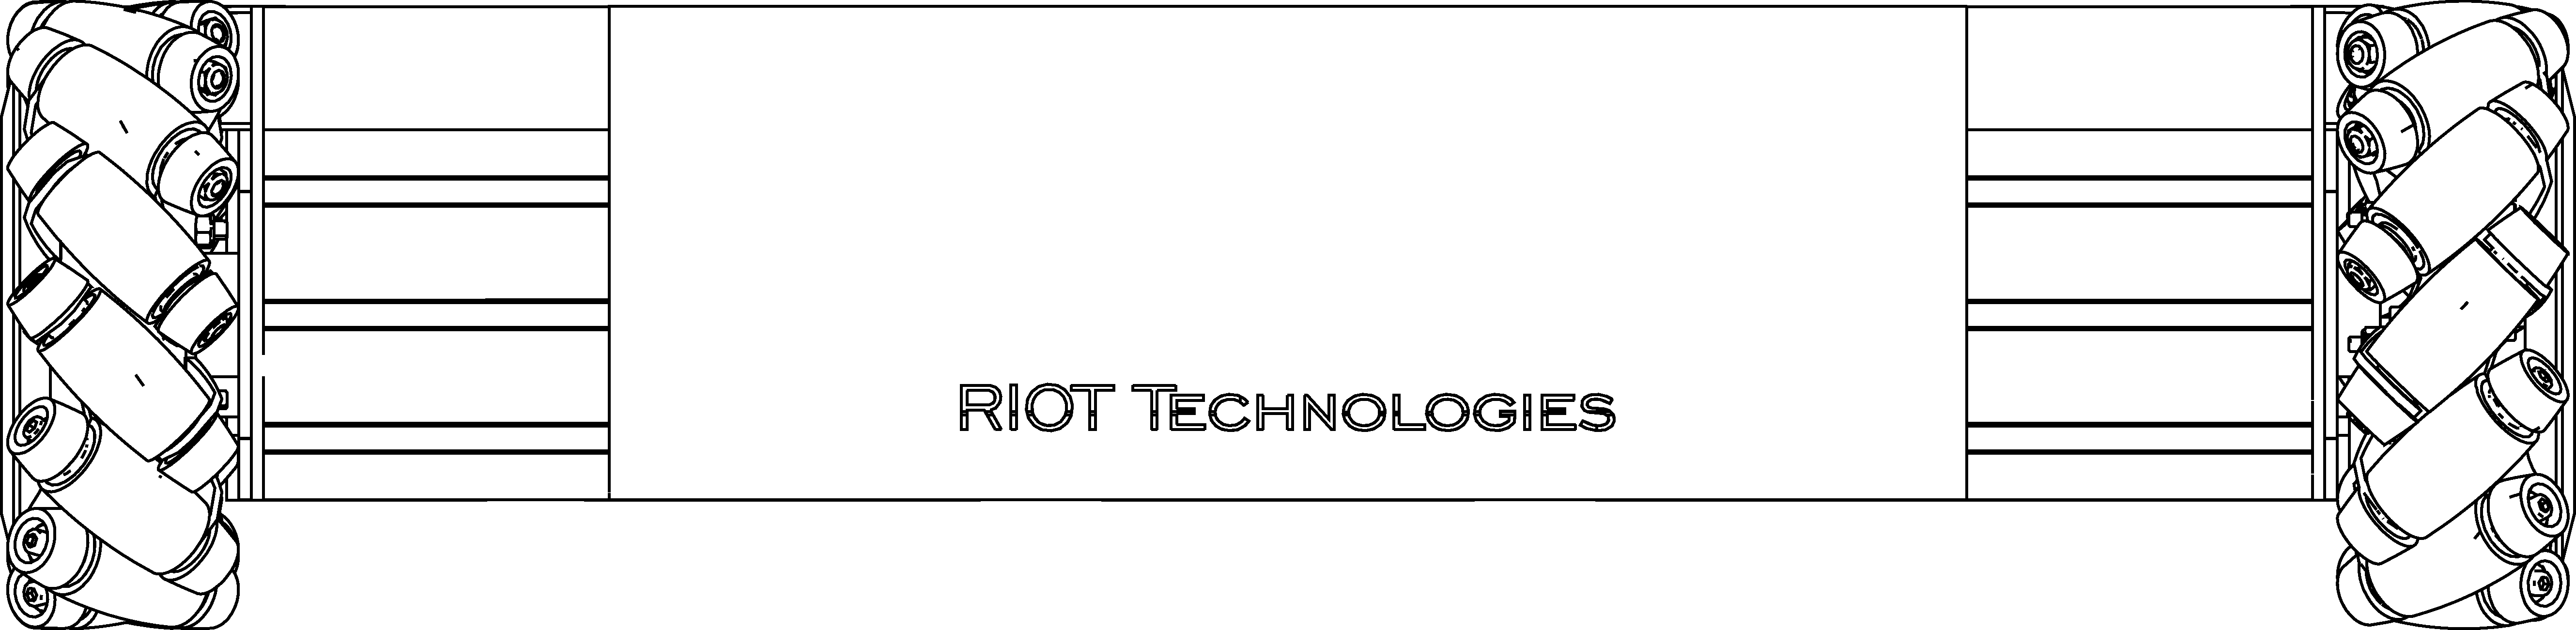
\includegraphics[width=0.5\textwidth]{graphics/base_front.pdf}
\caption{Platforma mobilna widziana od tyłu.}
\end{figure} 



\section{Składniki systemu}
Symulacja składa się z kilku odrębnych składników, które komunikują się ze sobą poprzez specjalne interfejsy oparte o kolejki wiadomości.
To pozwala zamieniać i przepisywać elementy zachowując tę samą komunikację między składnikami i nie tracąc kompatybilności.

\subsection{Model}
 Odpowiednio opisany równaniami powinien być jak najdokładniejszą kopią fizycznego robota.
 Musi brać pod uwagę masy i momenty bezwładności elementów składowych, a także możliwe tarcia.
 Model posiada także więzy na ruchome elementy, jak koła i rolki, aby obracały się w określony sposób.
 
 Ta część systemu oddziałuje bezpośrednio z silnikiem fizycznym. 
 To kształt, masy i momenty bezwładności brył są argumentami funkcji liczących.
 Także silnik manipuluje z powrotem podanymi obiektami nadając im odpowiednie prędkości w czasie.
 
 Do modelu doczepia się wirtualne czujniki generujące odpowiednie dane na podstawie symulacji i rozkładu losowego.
 Nie są to pełne dane o stanie modelu, jakie posiada silnik, gdyż w rzeczywistości również nigdy nie mamy pełnej informacji o stanie urządzenia.
 
 Dla ozdoby można mu nadać wygląd zbliżony do prawdziwego robota poprzez wymodelowanie siatki w programie graficznym i nałożeniu wymaganych materiałów.

 \subsection{Driver silników}
 Ma taką samą funkcjonalność, jak pokładowy driver niskopoziomowy na robocie.
 W rzeczywistości najczęściej implementowany w formie mikrokontrolera, lub podobnego systemu czasu rzeczywistego.
 Zadaniem pokładowego sterownika jest przyjęcie wartości sterowania od zewnętrznego programu i podanie odpowiednich wartości napięcia na silniki kół.
 Może także wprowadzać niezależne zabezpieczenia przed zniszczeniem urządzenia przez nieprawidłowe wejście.
 Taki program jest najczęściej dostarczony przez producenta robota i nie znany użytkownikowi.
 Zależy ściśle od budowy urządzenia i nie może być prosto wymienialny z innym obiektem.
 
 Cel polega na stworzeniu alternatywnego programu pobierającego podobne, co w fizycznej wersji dane i obracającego kołami w odpowiedni sposób.
 Tutaj polega to na wywoływaniu funkcji silnika fizycznego z odpowiednio przygotowanymi argumentami.
 Silnik fizyczny symulatora przekłada te siły na odpowiednie prędkości w przestrzeni wirtualnej biorąc pod uwagę charakterystykę modelu i otoczenia.
 
 \subsection{Driver czujników}
 Normalny driver na urządzeniu pobiera surowe dane i zamienia je na format możliwy do odczytania przez zewnętrzny program.
 Najczęściej polega to na próbkowaniu sygnału i wysyłaniu go dalej.
 Driver może także robić wstępne obrabianie danych w celach usuwania szumów, korekcji błędów, albo szybkiej obróbki na wyższy format, jak ma to miejsce na przykład w kamerze Kinect.
 
 Symulując ten element budujemy program generujący dane na podstawie aktualnego stanu symulacji. 
 W celu przybliżenia go do realizmu powinno także dodawać się do generowanych danych sztuczny szum i błędy, aby łatwiej można było go zamienić później na prawdziwy czujnik.
 
\subsection{Program sterujący}
 Cześć odpowiedzialna za logikę aplikacji. Tutaj podejmowane są decyzje, jakie wymusić prędkości kół, aby pojechać po wymaganej krzywej.
 Ten program także pobiera, obrabia i interpretuje przetworzone przez driver dane z czujników.
 
 W tej części używanych jest wiele zaawansowanych algorytmów, jak budowanie mapy, szukanie ścieżki, unikanie kolizji, wyznaczanie obiektów na obrazie itp.
 Zwykle działa to na dużych, wielowątkowych maszynach ze względu na spore wymagania obliczeniowe.
 Jeśli robot komunikuje się z użytkownikiem, to ma to miejsce tutaj.
 
 Sterownik składa się z wielu modułów, każdy odpowiedzialny za coś innego. Może być stworzony w językach wysokopoziomowych, a nawet po części skryptowych, gdyż nie ma wymagań czasowych.
 Zazwyczaj program ma wiele poziomów. Nadrzędne algorytmy decyzyjne wołają niższe funkcje odpowiedzialne np. za planowanie, a te z kolei jeszcze niższe od np. ruchu itp.

\section{Technologie}
Symulator daje użytkownikowi do dyspozycji odpowiedni silnik fizyczny w którym odbywa się symulacja modelu, oraz API do obsługi.
Zaawansowany silnik powinien obsługiwać odpowiednie tarcia, więzy, siły, materiały fizyczne i wszystko, co potrzebne do jak najwierniejszego odtworzenia prawdziwego zachowania obiektu.
Na rynku jest wiele różnych silników zarówno do symulacji w czasie rzeczywistym, jak i do wyznaczania tras obiektów po długich obliczeniach.
Jedne z technologii są otwartoźródłowe, inne mniej.

\subsection{Gazebo}
Ten silnik jest dość prosty w obsłudze i wydaje się mieć mało funkcji ze względu na prosty interfejs.
Jednak jego potencjał tkwi w argumentach linii poleceń i w czytaniu podanych plików.

Program symuluje podane obiekty używając jednego z czterech popularnych silników fizycznych: ODE, Bullet, Simbody lub DART.
Wszystkie te silniki są wolnym oprogramowaniem i używane także w innych programach, jak na przykład Blender.

Program oprócz symulatora ma wbudowany edytor modeli i budynków w którym możemy tworzyć nasze dzieła od razu w przestrzeni trójwymiarowej.
Jakość wykonania tych składników jest bardzo słaba, brak jest tak podstawowych funkcjonalności, jak cofanie ruchu.
Również tworząc modele w ten sposób nie mamy nad nimi pełnej kontroli i dokładności.

Zatem najlepszym sposobem jest tworzenie modelu w specjalnym formacie SDF. Jest to ustandaryzowany zdefiniowany zewnętrznie format do opisywania składników robotów i czujników.
Dzięki temu napisany w ten sposób model może być użyty także gdzie indziej, pod warunkiem przestrzegania standardu.
Składnia jest zwykłym plikiem XML, co znaczy, że może być tworzony na każdym edytorze tekstowym.

Wtyczka do sterowania modelem jest zwyczajną biblioteką dołączaną w czasie symulacji. 
Pisze się ją w C++ jako własna klasa dziedzicząca po klasie wtyczki Gazebo.
Dodatkowo tym sposobem może się łączyć z programem sterującym poprzez kolejki wiadomości udostępnione przez Gazebo, lub inne mechanizmy, nawet systemowe, jak gniazda, czy pamięć współdzielona.

Program działa domyślnie na dystrybucji Ubuntu, ale bez problemu można go także skompilować pod inne systemy.
Interfejs jest dopracowany i przestrzega wielu ustawień systemowych, jak DPI.
Uruchamianie jest proste i nie wymaga dodatkowych ustawień, tworzenia odpowiednich katalogów, czy definiowania zmiennych systemowych.
Podobnie do wszystkich tworzy ukryty katalog w katalogu domowym użytkownika, gdzie znajdują się wszystkie modele i logi.

\subsection{V-Rep}
Duży i skomplikowany silnik reklamujący się wieloma zaawansowanymi mechanizmami.
Bogaty interfejs graficzny zakłada budowę i symulację wszystkiego w tym jednym programie.

Używa dwóch z silników z Gazebo, czyli ODE i Bullet, oraz Vortex i Newton. Z tej czwórki tylko Vortex ma zamknięty kod.
Podobno symulacja fizyczna jest gorszej jakości, niż w Gazebo.

Problemem jest także zapisywanie utworzonych w programie modeli.
Program zapisuje drzewiastą strukturę modelu w pliku binarnym własnego formatu, co uniemożliwia edycję i oglądanie modelu bez posiadania całego programu i wczytywania pliku.
Brak przenośności, czy wsparcia kontroli wersji dla takich zbiorów bajtów także jest problemem.

Pisanie wtyczek najczęściej odbywa się w C. Są też dostępne inne języki skryptowe, jak Lua, Matlab, Java itp.
Komunikacja z innymi programami odbywa się poprzez specjalne mosty w formie dodatków.
API pozwala nam stworzyć mały interfejs graficzny do sterownia symulacją poprzez przyciski i suwaki.

Ze strony producenta pobieramy gotowe archiwum z programem, który nie wymaga żadnej instalacji i posiada wszystkie potrzebne zasoby do pracy i nauki, jak przykładowe modele istniejących komercyjnych robotów.
Program działa na trzech Najpopularniejszych systemach operacyjnych --- Windows, Linux i OS X.

Lepiej jednak jest używać do symulacji Gazebo głównie ze względu na jego otwartość, prostotę i elastyczność.

\subsection{ROS}
Najpopularniejsza biblioteka i gotowe algorytmy do budowania logiki sterowania.
Dostępne są tutaj programy do obróbki danych, wyznaczania ścieżek, tworzenia map itp.

Właściwie nie ma dobrej alternatywy do zbioru tych bibliotek, poza implementacją wszystkiego ręcznie na nowo i po swojemu.
Programy dla ROS pisze się w C++ i integruje z robotem za pomocą kilku gotowych struktur.

Instalacja programu na komputerze jest dużym problemem.
Z wyjątkiem Ubuntu nie ma łatwego sposobu na wgranie go do innych systemów.
Na przeszkodzie stoją błędy kompilacji dla nowszych wersji kompilatorów i inne problemy wykonania, jak naruszenie ochrony pamięci. 
Niektórym studentom wydziału się udało tego z wielkim trudem dokonać, lecz dużo prościej jest użyć Ubuntu na maszynie wirtualnej, bądź dysku USB.
Takie rozwiązanie także daje dostęp do najnowszej wersji \emph{Kinetic Kame} niedostępnej jeszcze na innych dystrybucjach.

Uruchomienie systemu wymaga wielu dodatkowych komend inicjalizujących, a także dopisywania wielu plików konfiguracyjnych za pomocą wielu skryptów do tworzonych projektów.
Używanie linii poleceń wymaga ustawienia kilku zmiennych systemowych.
Użycie niektórych funkcji wymaga uruchomionego demona serwera w tle.
Ogólnie instalacja i używanie ROS na systemie dużo śmieci, dlatego lepiej jest trzymać ją z dala od codziennego systemu operacyjnego na maszynie wirtualnej, lub dysku.

\section{Ogólny zarys pracy}
\begin{enumerate}
 \item Należy stworzyć model w SDF zachowując wszystkie rozmiary i momenty prawdziwego robota.
Należy ustawić bryły, aby przypominały kształtem podstawę i nadać im parametry fizyki.

\item Trzeba zdefiniować wszystkie więzy na koła i przegub i zamodelować je, aby silnik fizyczny dobrze współpracował.
Taki model powinien na tym stanie reagować na zewnętrzne siły, ale nie ruszać się własnymi silnikami.
Można go prosto przetestować działając siłą na elementy i patrząc, czy reaguje w poprawny sposób.

\item Wtyczka sterująca w Gazebo odczytuje dane z zewnątrz i odpowiednio obraca kołami.
Na tym poziomie można dobudować zamiennik programu sterującego jedynie do podawania prostego sterowania na koła, bez żadnej logiki.
Do komunikacji użyć struktur Gazebo, a nie ROS.
Model powinien poprawnie reagować na proste wejście, jak naprzemienne koła itp.

\item Wtyczki dla czujników, aby generowały dane z enkoderów, oraz ewentualnie innych urządzeń, dodawały błędy pomiarowe i wysyłały je na zewnątrz, aby program sterujący miał dane do działania.
Taki model jest w tym momencie kopią prawdziwego robota.

\item Program sterujący w ROS. Największy i najbardziej skomplikowany element, na szczęście wspólny dla obu bytów --- wirtualnego i rzeczywistego.
Zazwyczaj nie jest to praca jednego człowieka, a jego rozwój nie ustaje przez długi czas.
Ten program dostarczy funkcji ruchów wywoływanych przez wyższy sterownik Velmy.

\end{enumerate}

\section{Pomocne implementacje}
Istnieją już wcześniejsze modele jeżdżących robotów na kołach szwedzkich.
Można z nich brać przykład i sugerować się źródłami kodu i modelów.

Kuka Youbot jest popularnym robotem tego typu. Jego modele są domyślnie dostępne zarówno w Gazebo, jak i w V-Rep.
Tylko w przypadku V-Rep mamy wstępny sterownik do którego kierujemy zadane prędkości kół za pomocą graficznego interfejsu.
Wersja dla Gazebo symuluje kłodę drewna.

Te profesjonalne modele także pomogą przy wstępnej weryfikacji zachowania się naszego modelu, czy nie zachowuje się nadzwyczaj dziwnie.

\chapter{Budowa bazy}
\label{sec:robot}
\section{Dookólna platforma mobilna}
	\begin{figure}[H]
	\centering
	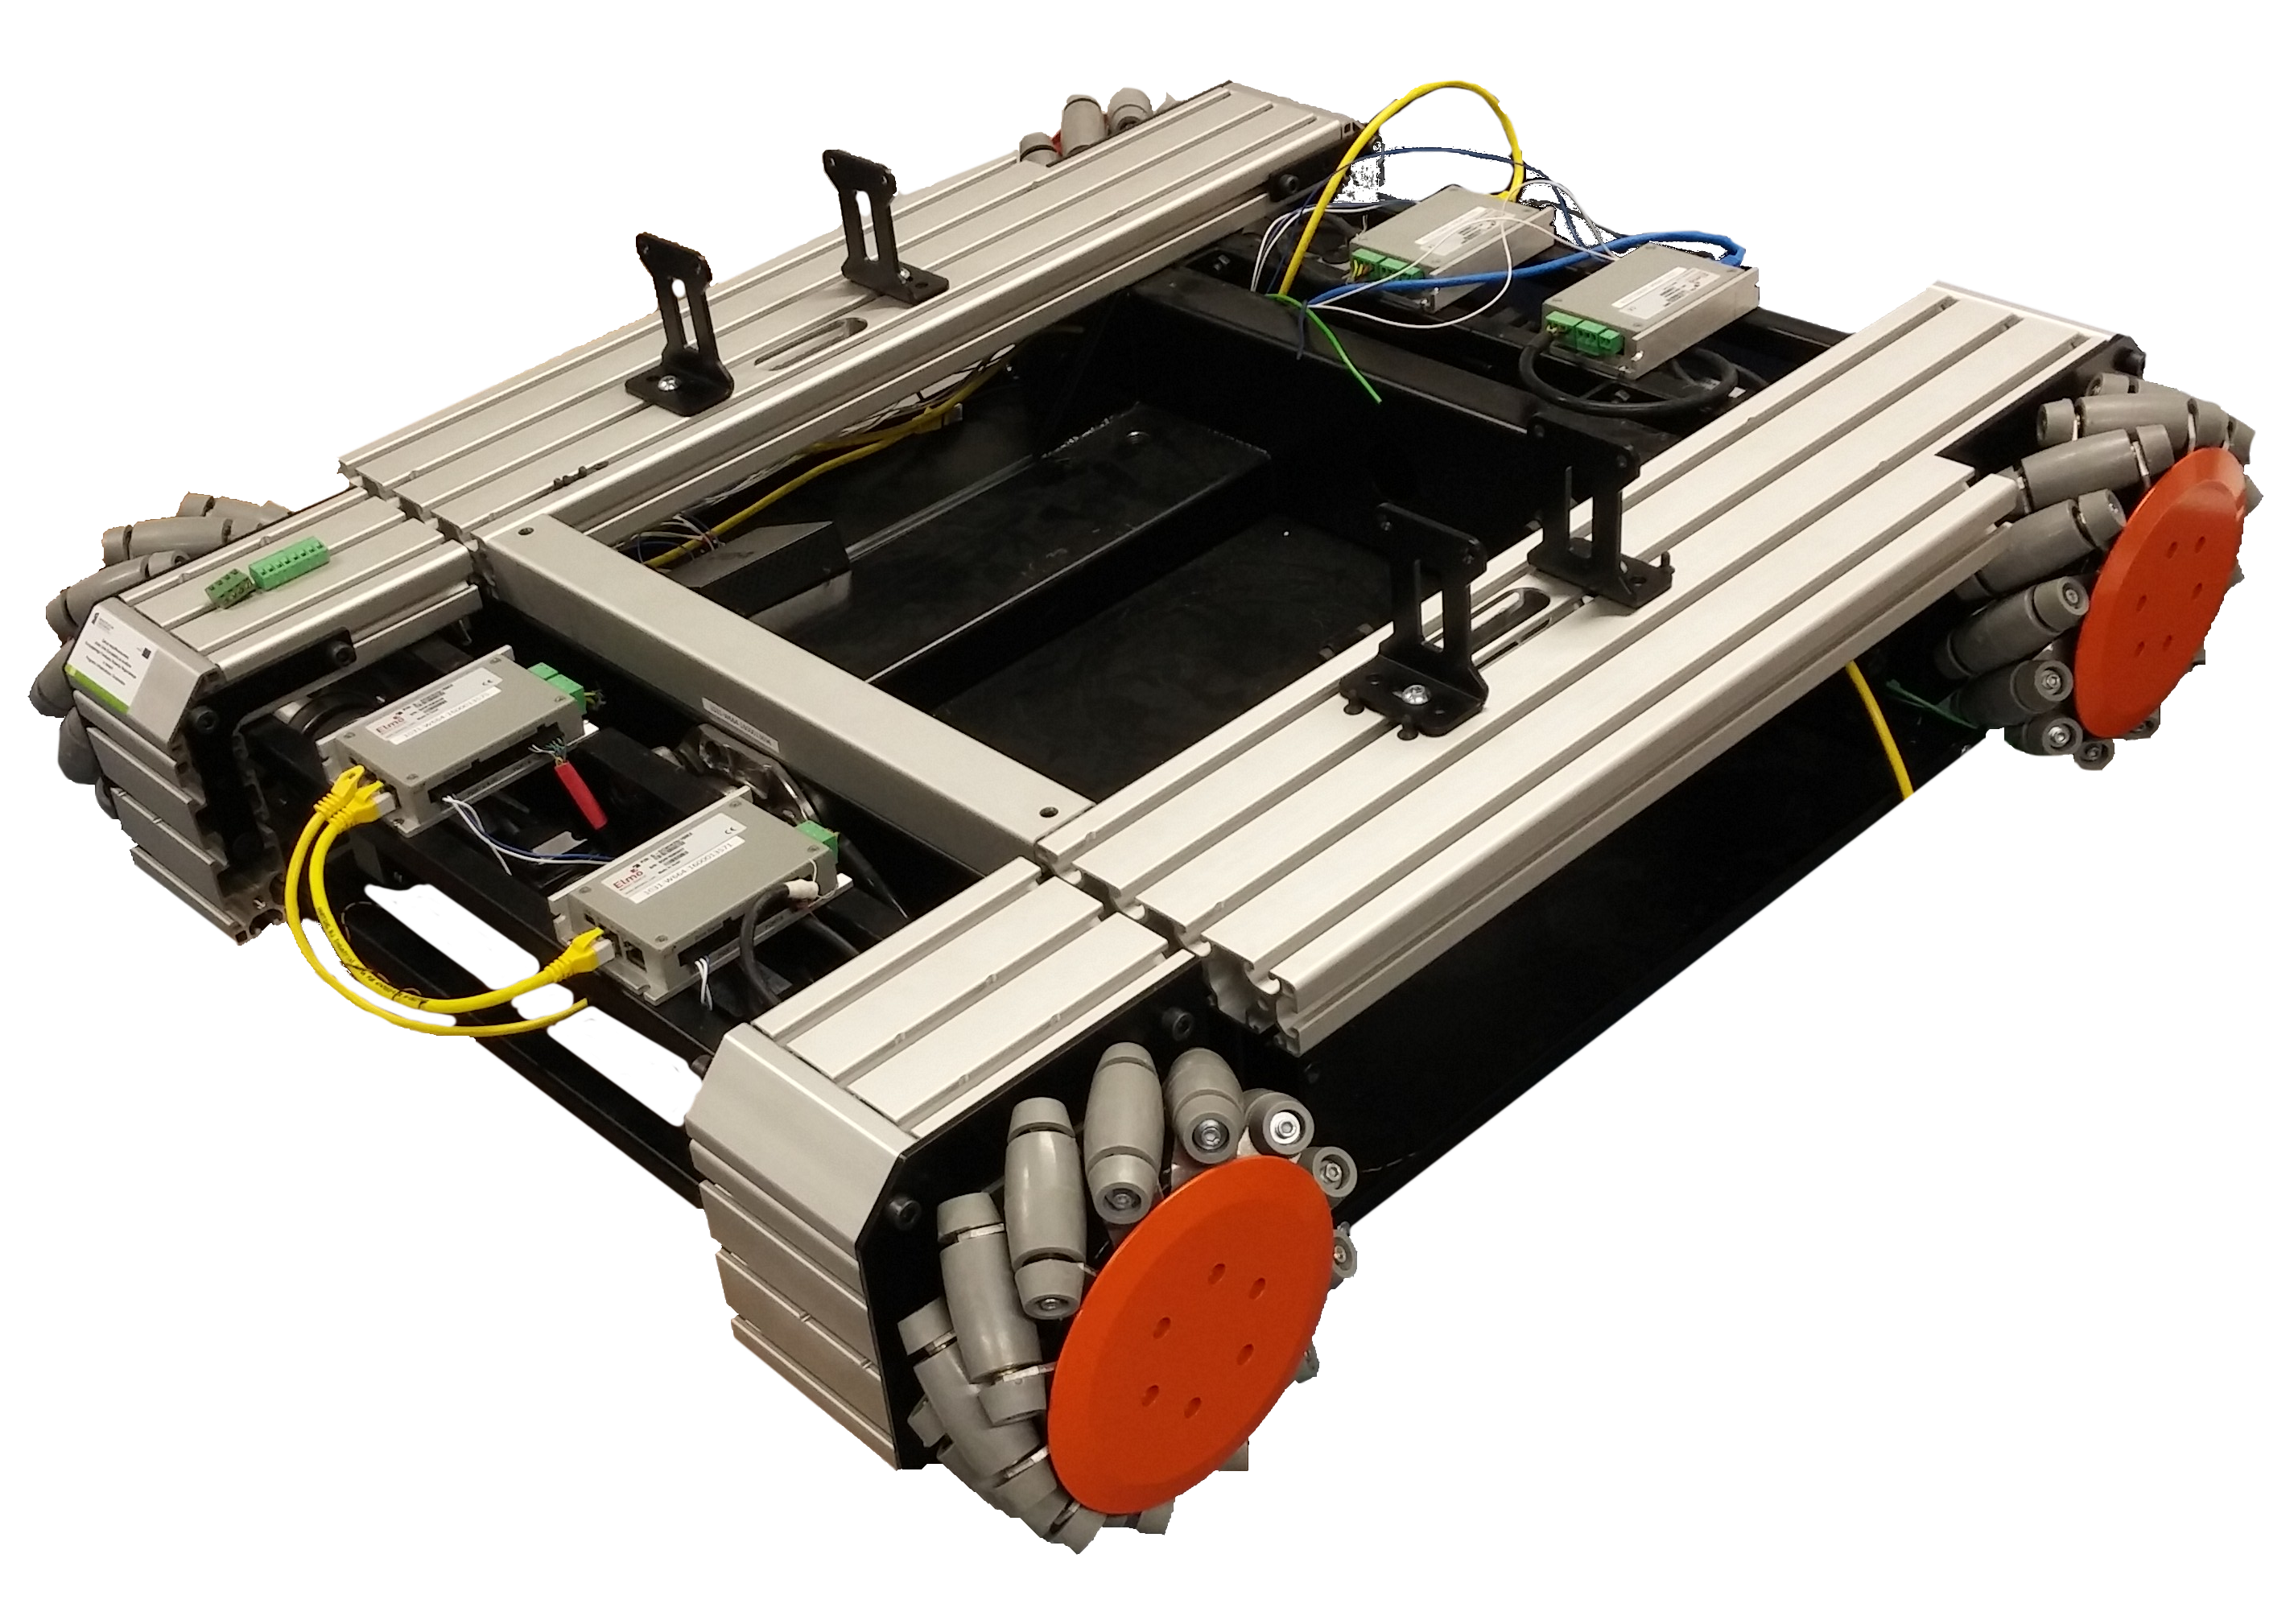
\includegraphics[width=0.8\textwidth]{graphics/base_photo.png}
	\caption{Dookólna baza mobilna na kołach szwedzkich.}
	\label{fig:base_photo}
	\end{figure} 

	Jest to duża, prostokątna baza dookólna, poruszająca się na czterech kołach szwedzkich, rysunek \ref{fig:base_photo}.
	Koła są stałe, parami przytwierdzone do dwóch osi.
	Każde koło jest napędzane osobno przez podłączony bezpośrednio serwomotor, 
	zatem może mieć prędkość i kierunek obrotu niezależny od pozostałych kół, kierunku poruszania się robota, oraz jego orientacji.
	Każdy z serwomotorów ma także wbudowany enkoder.
	Sterownik enkodera nadaje za pomocą sieci aktualny kąt i prędkość obrotu.

	Jest to jeden z najpopularniejszych typów dookólnych platform mobilnych, mających zastosowanie także w innych robotach, jak na przykład Kuka Youbot, rysunek \ref{fig:kuka_youbot}.
	Należy zwrócić uwagę na charakterystyczne ustawienie kół, identyczne jak w opisywanej platformie na rysunku \ref{fig:base_photo}.
	
	Istnieją także roboty z trzema kołami szwedzkimi, w których koła rozstawione są na wierzchołkach trójkąta równobocznego.
	Pomimo prostszej budowy i takiej samej liczby stopni swobody, jak czterokołowa wersja, stabilność takiej konstrukcji jest gorsza \cite{extra_axis}.
	Ponieważ jest to robot transportowy, to stabilność odgrywa tu ważną rolę i czterokołowa konstrukcja jest wskazana.

	\begin{figure}[H]
	\centering
	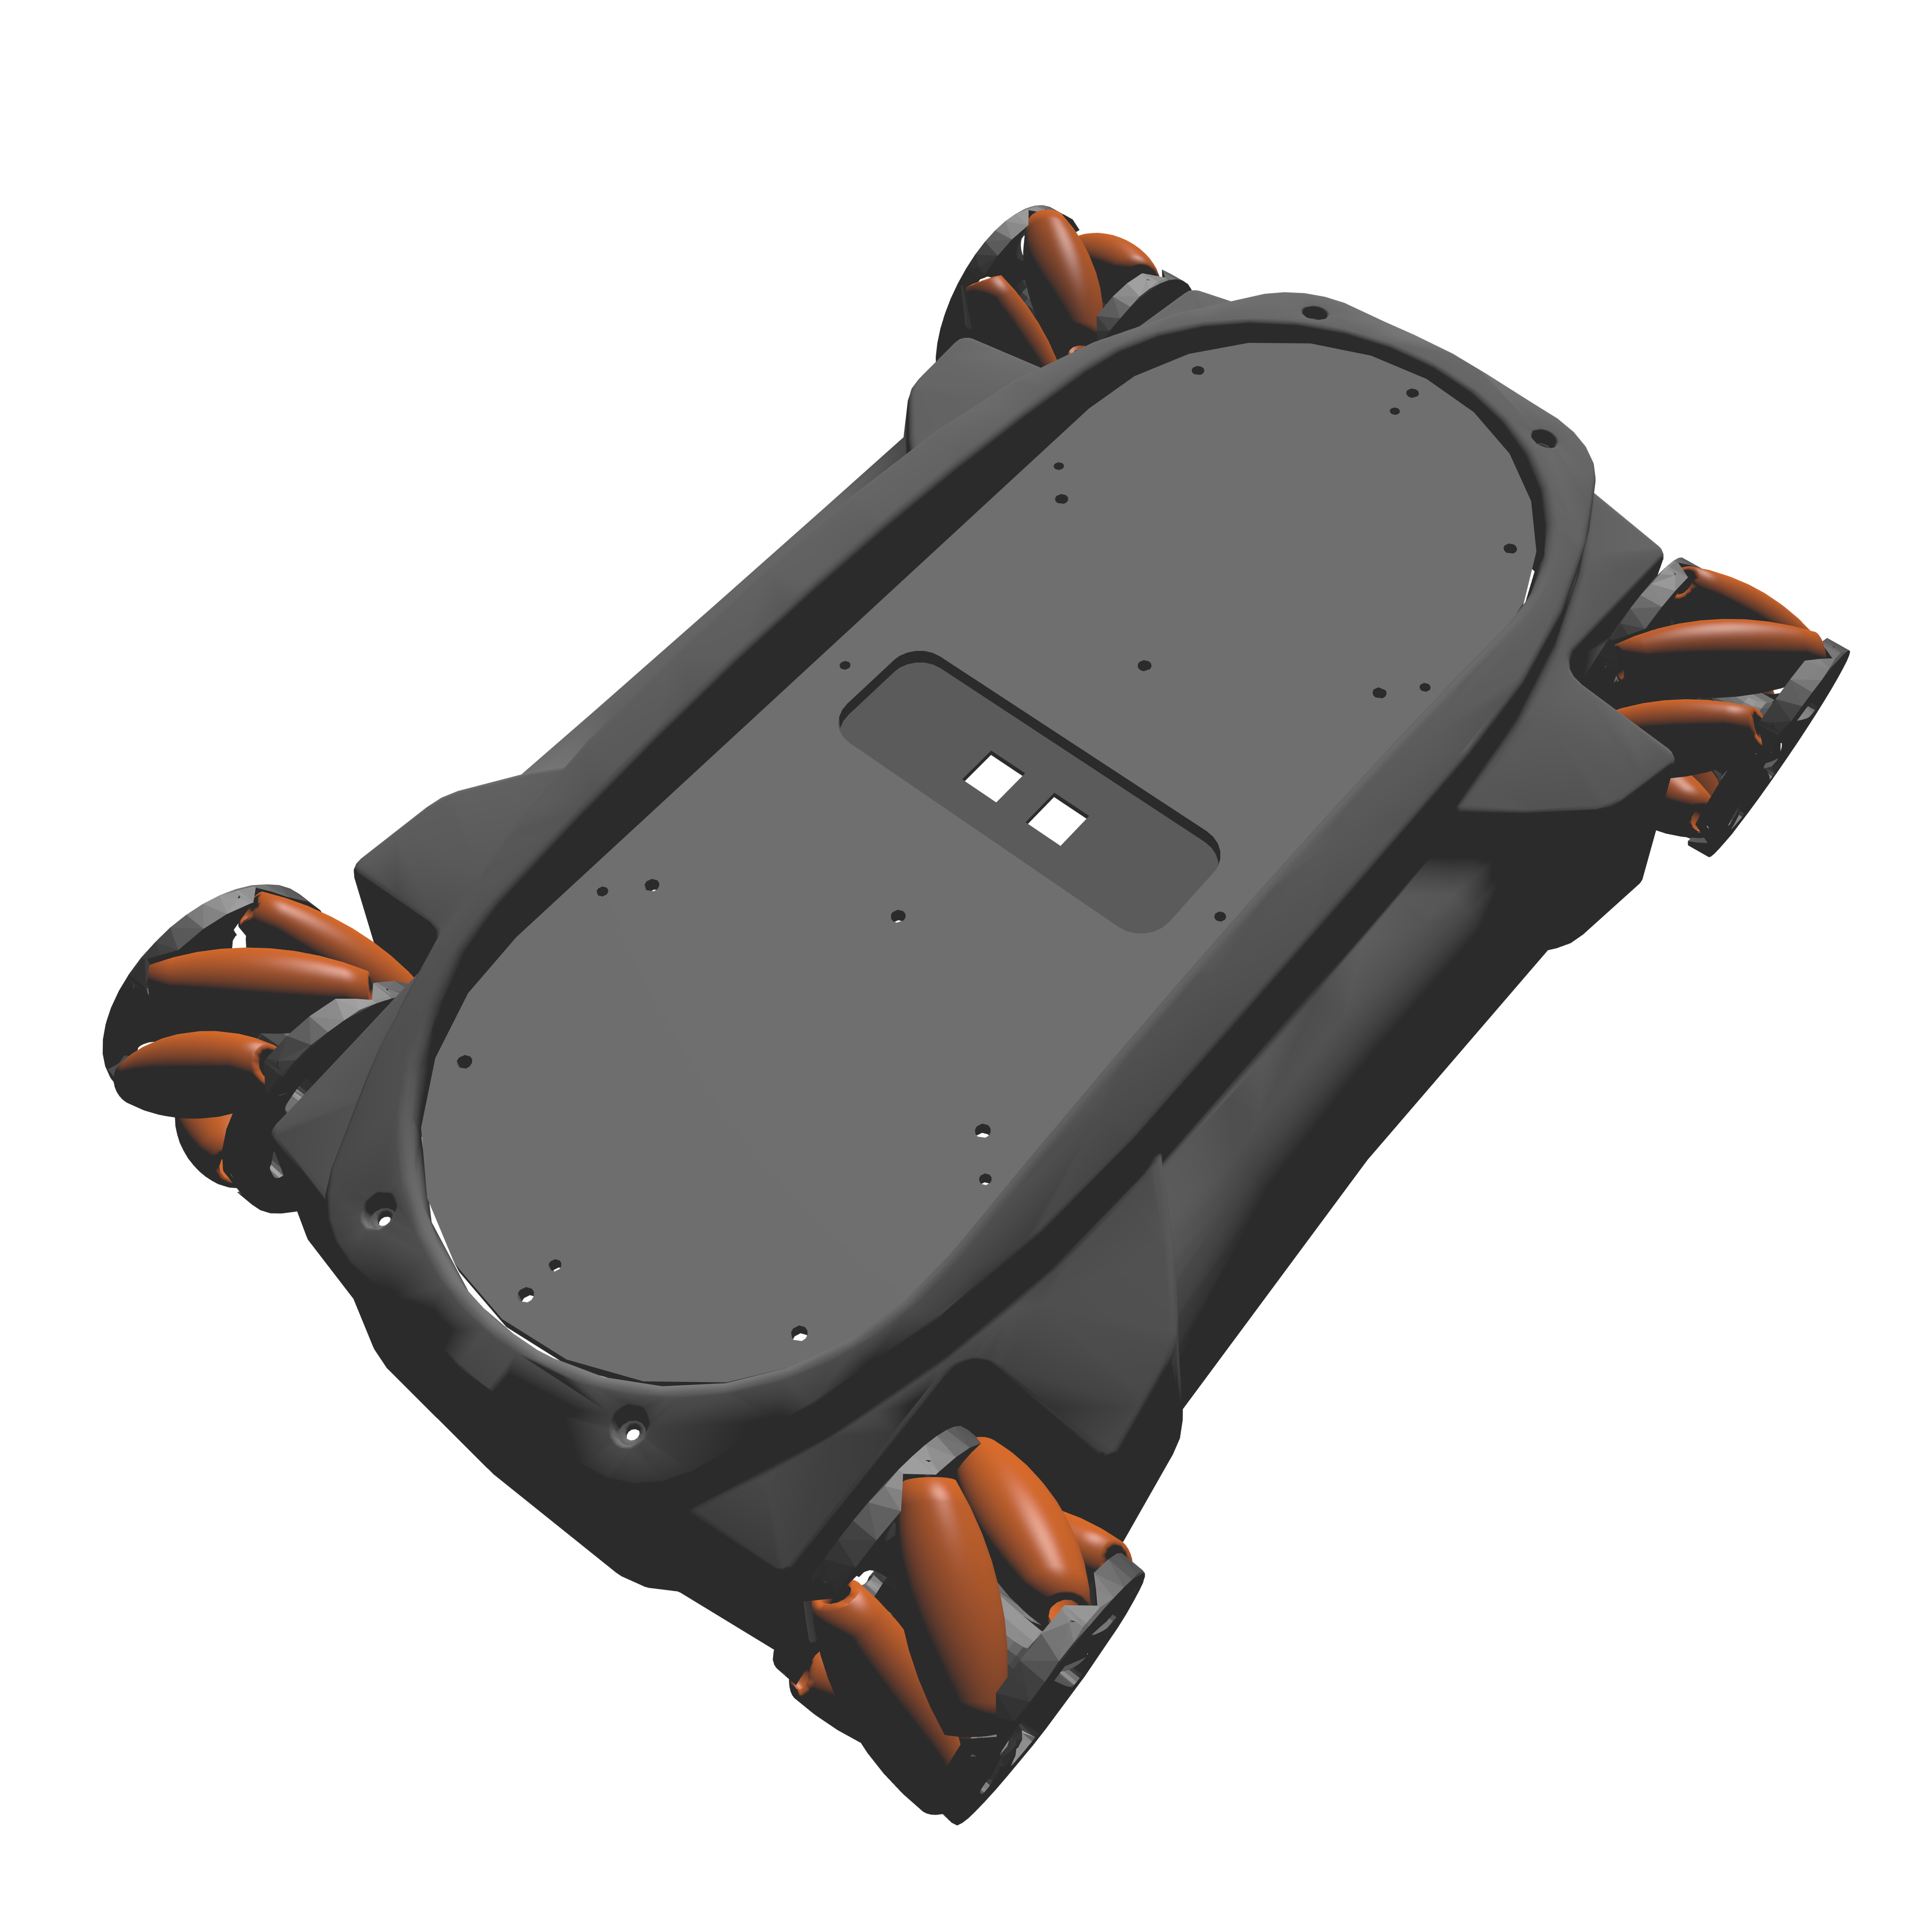
\includegraphics[width=0.5\textwidth]{graphics/kuka_youbot.png}
	\caption{Platforma wycofanego już ze sprzedaży robota Kuka Youbot.}
	\label{fig:kuka_youbot}
	\end{figure} 

	Odpowiedni obrót kół względem bazy, pozwala na jej ruch w dowolnym kierunku, niezależnym od orientacji robota, patrz rysunek \ref{fig:mecanum_dirs}.
	Jest możliwe także obracanie bazą, gdy ta porusza się w dowolnym kierunku, bądź stoi w miejscu.
	
	\begin{figure}[H]
	\centering
	
\includegraphics[width=0.8\textwidth]{graphics/mecanum_dirs.pdf}
	\caption{Podstawowe kierunki ruchu robota o napędzie wielokierunkowym.}
	\label{fig:mecanum_dirs}
	\end{figure} 
	
	Przykładowo, poruszając tylko przeciwległymi kołami po przekątnej, robot będzie mógł poruszać się po skosie, bez zmiany orientacji bazy.
	A jeśli do tego dodać obrót kół drugiej przekątnej, w odwrotnym kierunku, wtedy pojazd zacznie się poruszać w bok, pomimo faktu, że koła nie są skrętne i 
	nie mogą ustawić się zgodnie z kierunkiem jazdy.
	Trasa, po której porusza się robot, przy stałej prędkości kół, zawsze jest łukiem okręgu. W szczególnym przypadku można uznać prostą za okrąg o nieskończonym promieniu, a punkt za okręg o zerowym. 
	Wynika to z faktu, że każdy obiekt, który ma jednostajną prędkość i stały kierunek w lokalnym układzie współrzędnych oraz stałą prędkość kątową, będzie się poruszał po łuku.
	Zależność tego promienia okręgu $R$ od prędkości liniowej $v$ i prędkości kątowej $\omega$, wyraża się wzorem $R = \frac{v}{\omega}$.

	Baza mobilna będzie podstawą robota manipulującego Velma, tworząc razem manipulator mobilny.
	Velma to dwuramienny robot, wyposażony w dwa chwytaki o wielu przegubach, patrz rysunek \ref{fig:velma}.
	Taka budowa wymaga szerokiej podstawy, aby zachować bezpieczną równowagę całości.
	Jeżdżąc na tej bazie, robot może się przemieszczać i obracać w dowolnym kierunku, aby uzyskać lepszy dostęp do manipulowanych obiektów.

	\begin{figure}[H]
	\centering
	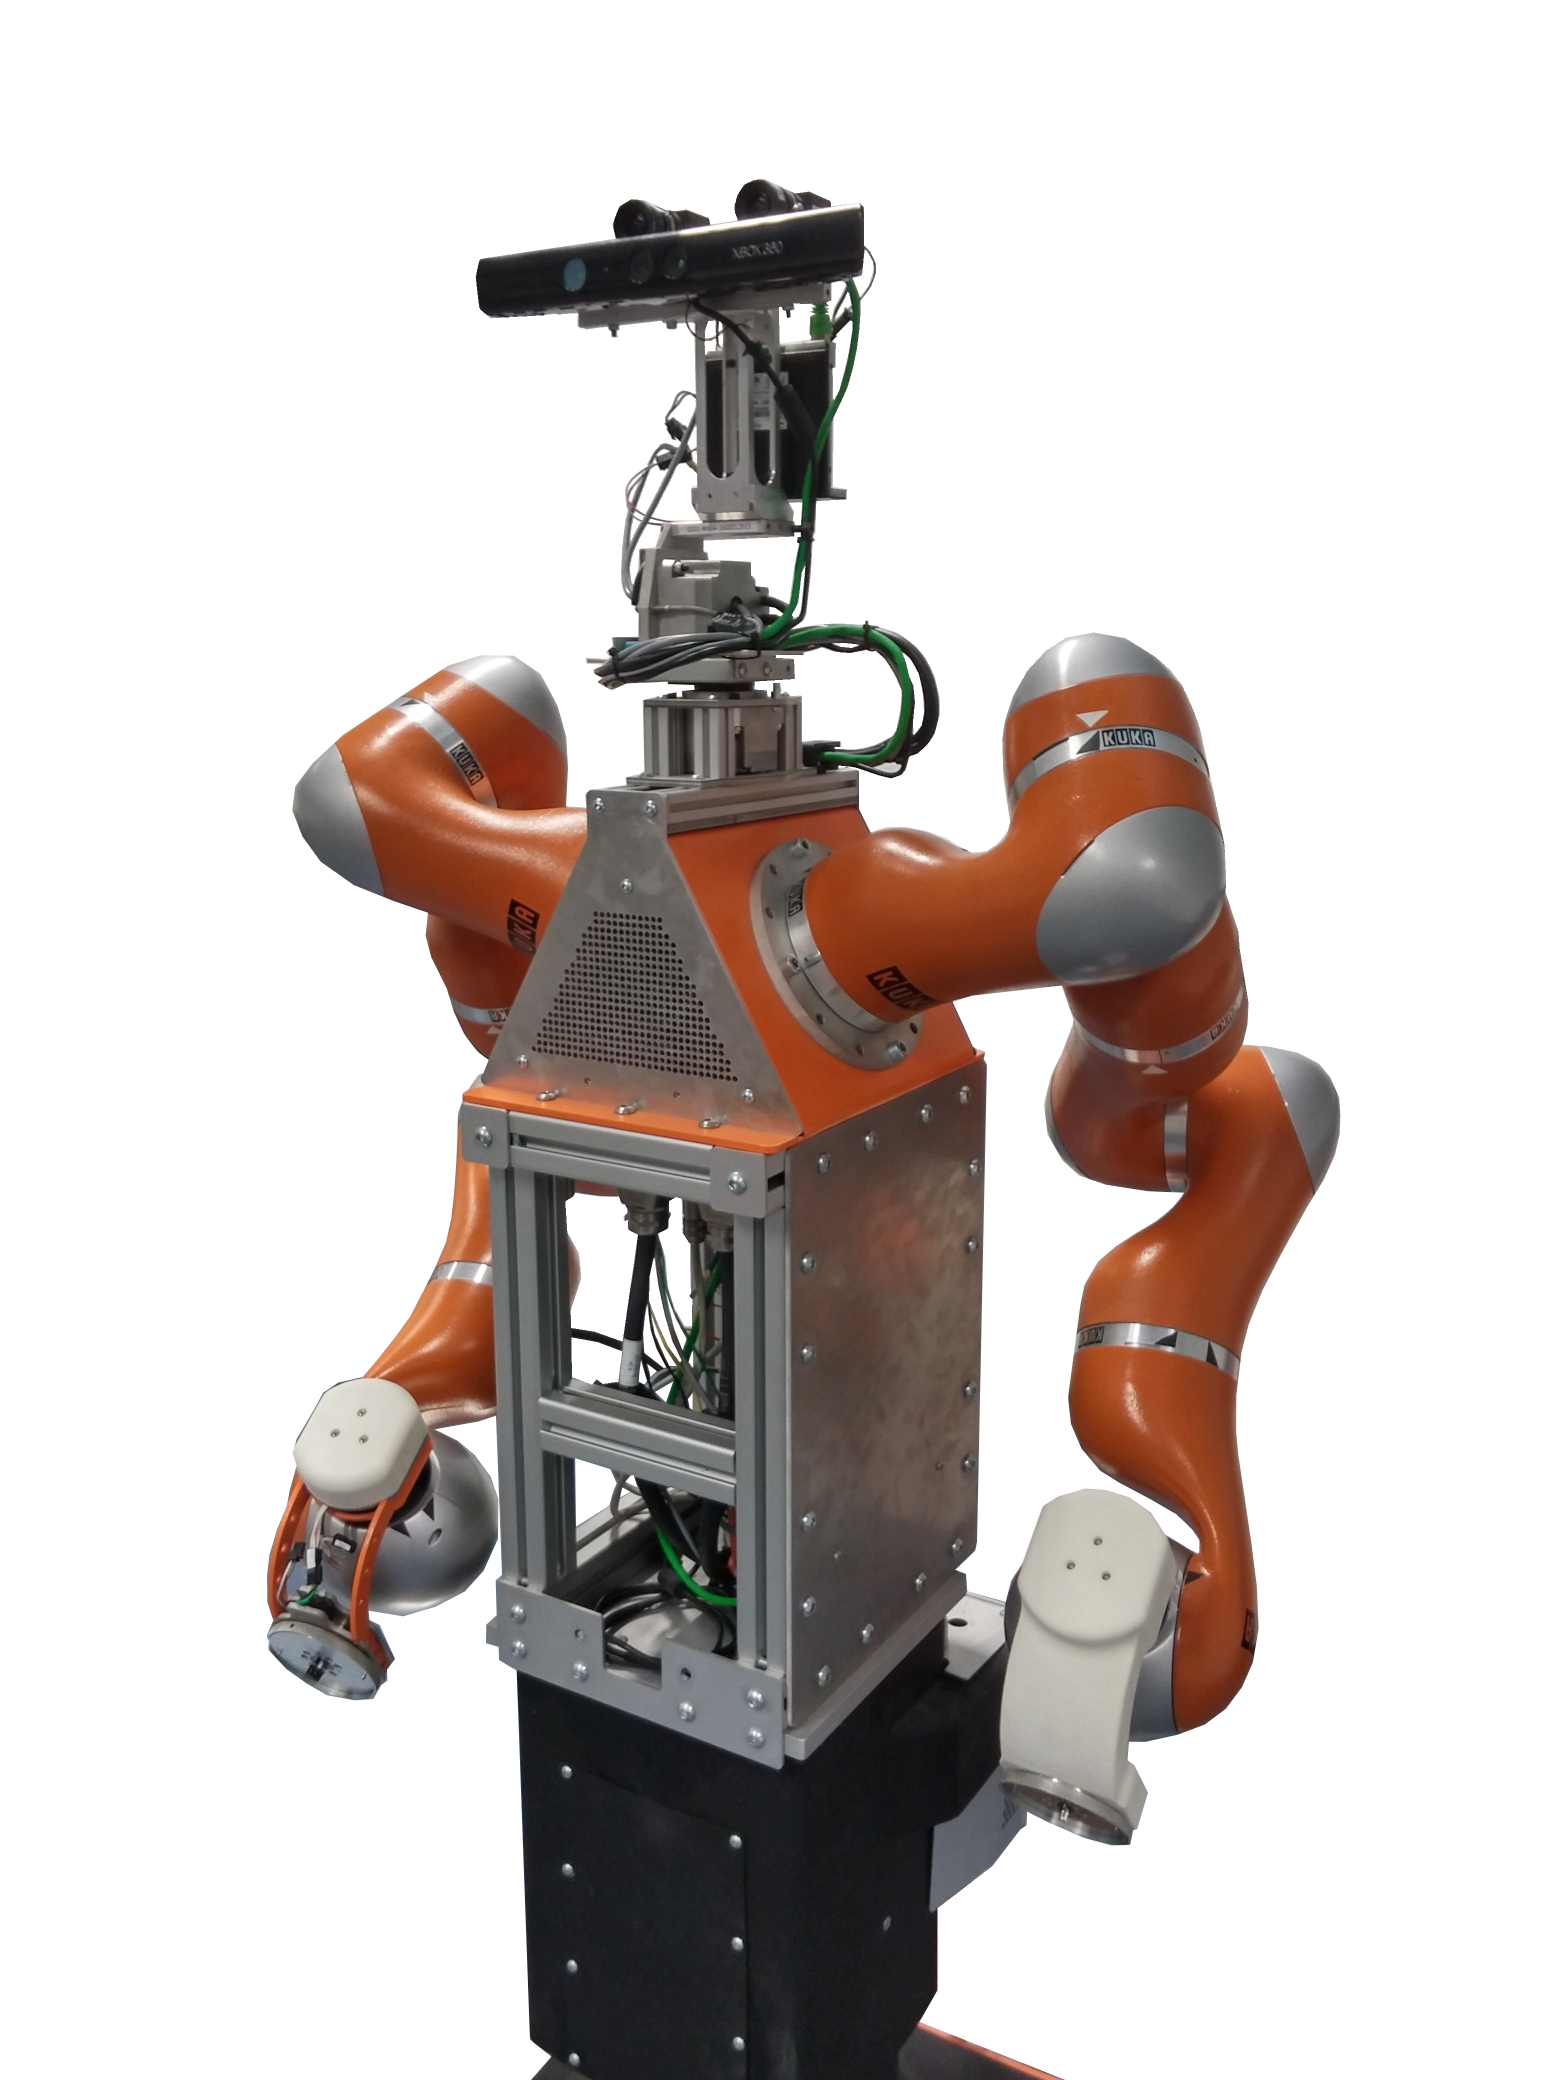
\includegraphics[width=0.5\textwidth]{graphics/velma.png}
	\caption{Robot manipulacyjny Velma.}
	\label{fig:velma}
	\end{figure} 

	Platforma jest niesymetrycznie podzielona na dwie części, przednią i tylną, w sposób pokazany na rysunku \ref{fig:base_ortho}.
	Przegub o jednym stopniu swobody (tzw. zawias) jest jedynym łącznikiem pomiędzy tymi dwoma fragmentami.
	Zadaniem tego przegubu jest zmniejszanie wpływu nierówności podłoża na ruch bazy, aby każde koło zachowało stały kontakt z podłożem.
	Bez tego przegubu, ruch po nierównym terenie uniemożliwiałby sprawne sterowanie platformą na skutek nieprzewidywalnych zaników tarcia kół o podłoże, powodując nieplanowane skręty.
	Takie zaniki tarcia kół są niewykrywalne w bezpośredni sposób, jak to zostało opisane w \cite{boringbot}.

	Platforma ma kształt prostokąta, jest 4 cm różnicy między szerokością, a długością robota.
	Koła są ustawione w wierzchołkach tego prostokąta.
	Szerokość jest większa, co można zobaczyć porównując widok z prawej strony, z widokiem z tyłu, rysunek \ref{fig:base_ortho}.
	Dokładne wymiary są podane na rysunku \ref{fig:base_dims} i tabeli \ref{tab:dims}.

	Platforma może w trakcie hamowania poruszać się innym kierunku, niż tuż przed zatrzymaniem.
	Jest to spowodowane tym, że konstrukcja rolek powoduje poślizg platformy w kierunku rolki mającej aktualnie kontakt z podłożem, a ten kierunek zależy od aktualnej
	orientacji bazy, nie od kierunku w jakim się porusza.
	Należy także wziąć tutaj pod uwagę inne cechy budowy kół, jak nierówne tarcie poszczególnych rolek o powierzchnię, 
	które może obrócić ten kierunek hamowania w nieprzewidywalny sposób \cite{braking}.

	\begin{figure}[H]
	\centering
	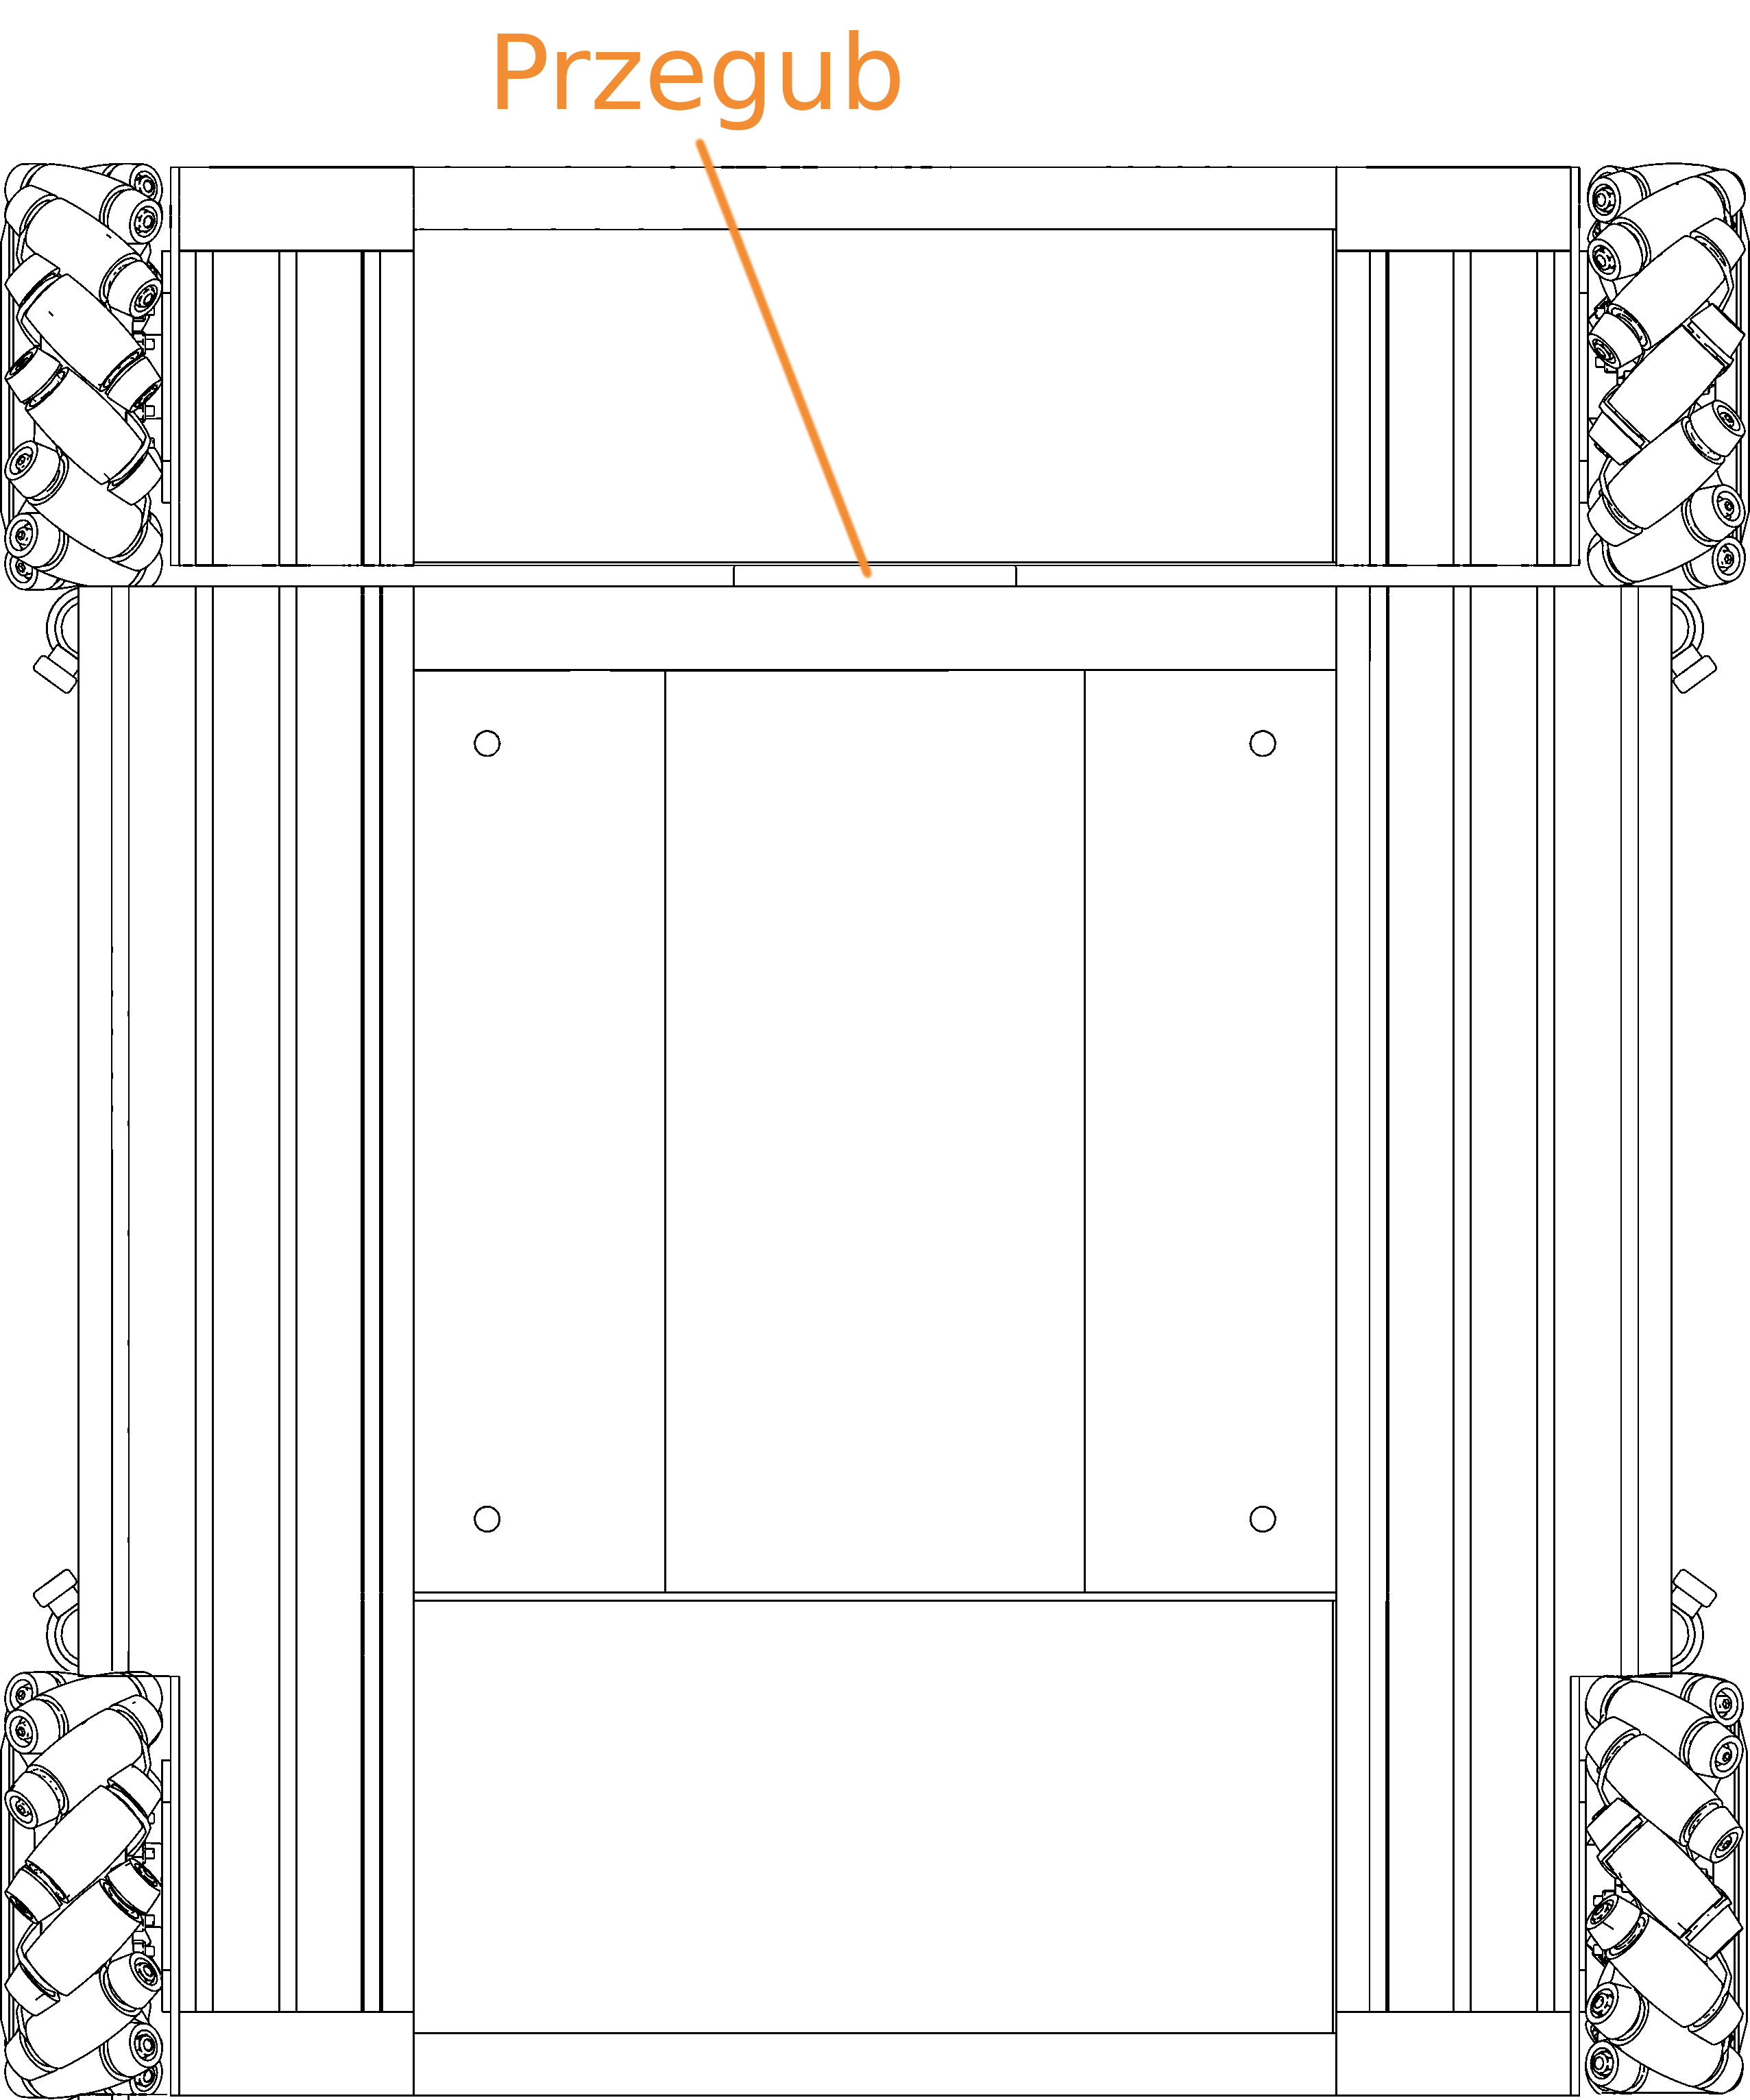
\includegraphics[width=0.5\textwidth]{graphics/base_top.png}
	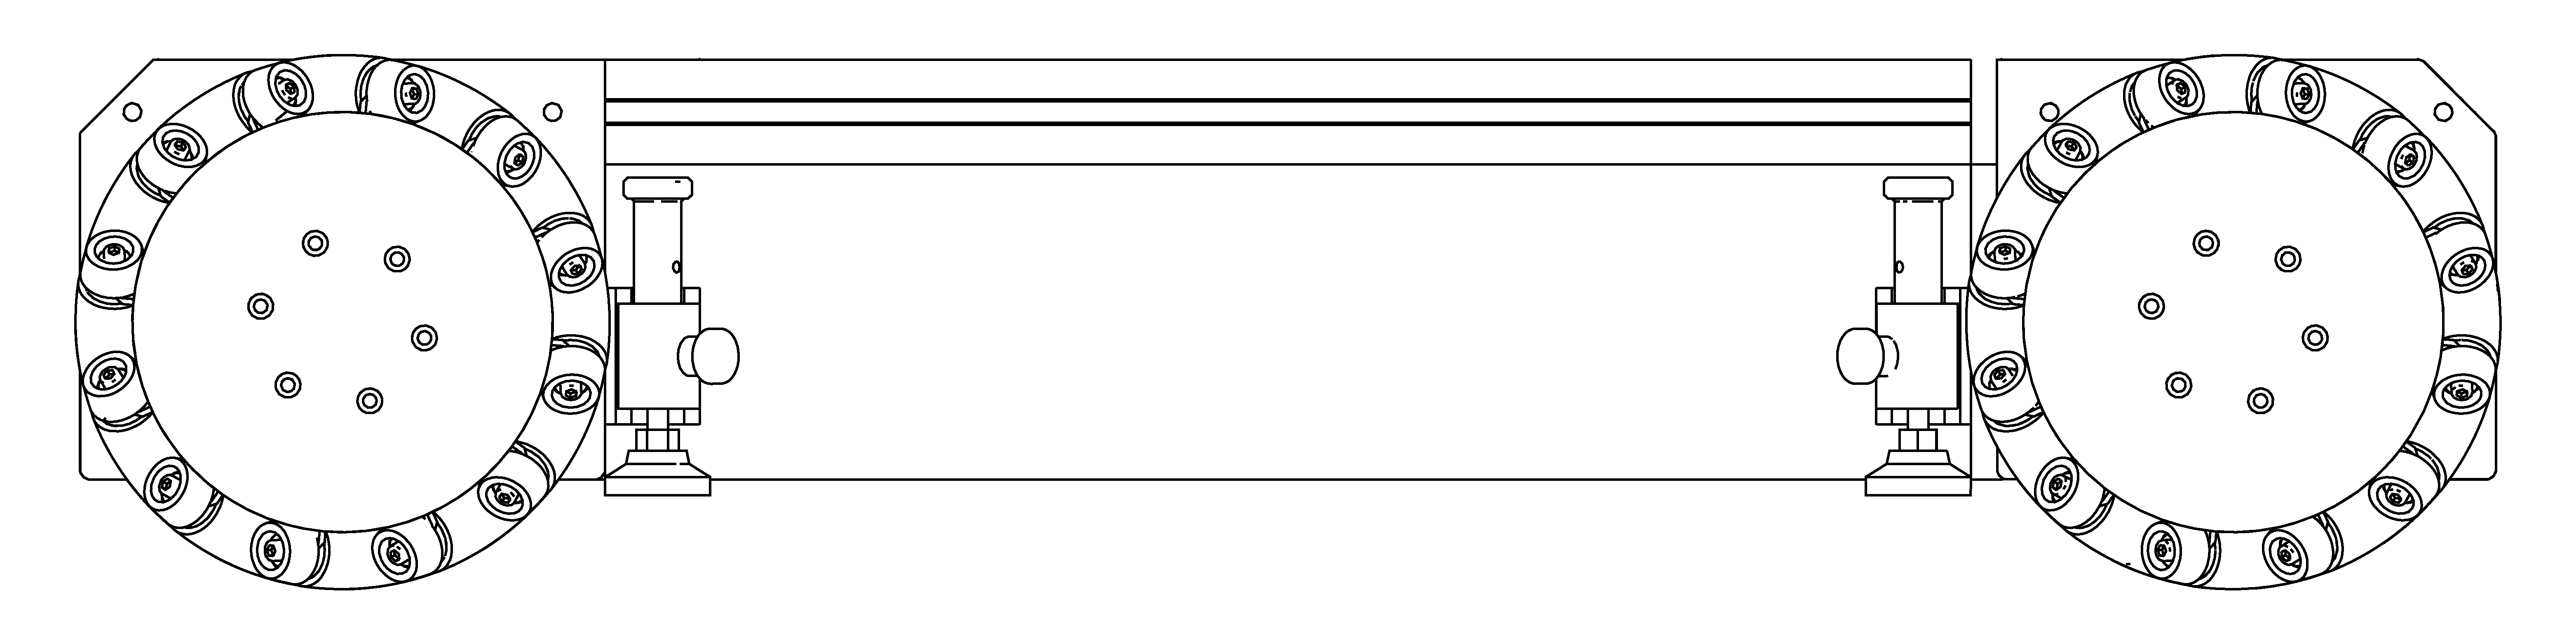
\includegraphics[width=0.62\textwidth]{graphics/base_side.pdf}
	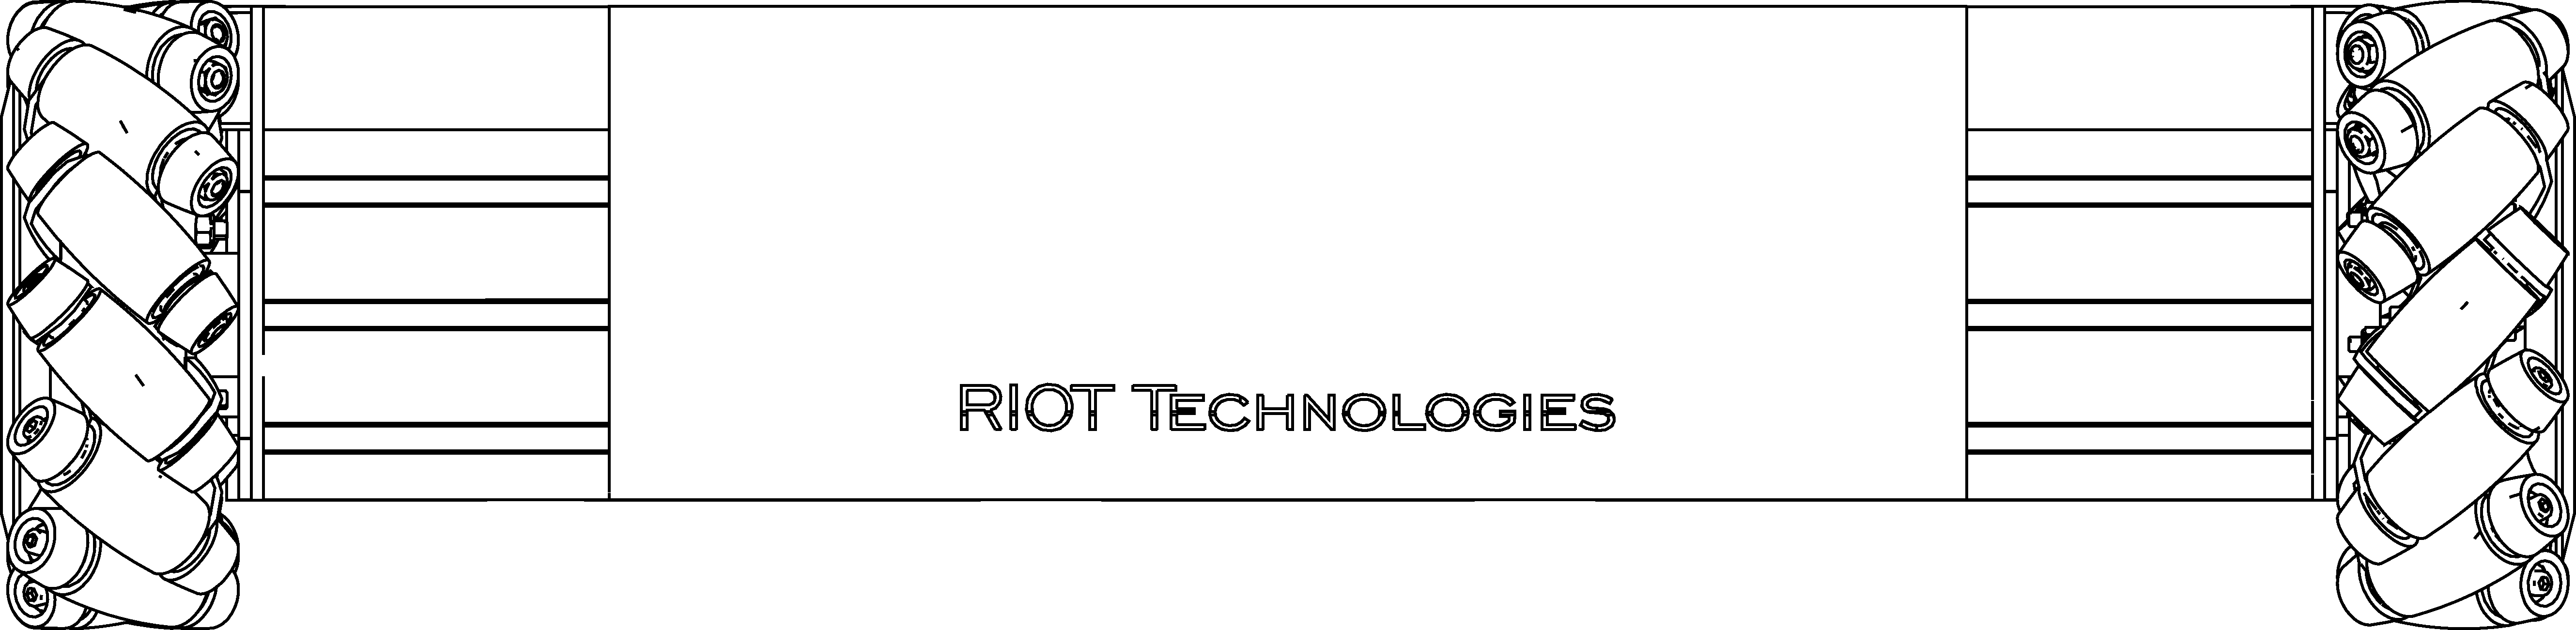
\includegraphics[width=0.62\textwidth]{graphics/base_front.pdf}
	\caption{Platforma mobilna. Widoki od góry, od prawej strony i od tyłu. Przegub obrotowy łączy dwie części.}
	\label{fig:base_ortho}
	\end{figure} 

	Platforma ma 3 stopnie swobody. 
	\begin{itemize}
		\item Przesunięcie wzdłuż osi X.
		\item Przesunięcie wzdłuż osi Y.
		\item Obrót wokół osi prostopadłej do podłoża.
	\end{itemize}
	
	Kierunek osi X i Y jest zgodny z ustalonymi dla programów sterujących platformą.
	
	\begin{figure}[H]
		\centering
		\includegraphics[width=0.8\textwidth]{graphics/base_dims.pdf}
		\caption{Wielkości używane we wzorach.}
		\label{fig:base_dims}
	\end{figure} 

	\begin{table}
		\centering
		\begin{tabular}{c c l}
		Oznaczenie & Wartość & Opis \\
		\hline
		$r$ & 0,1 m & Promień koła. \\
		$a$ & 0,76 m & Rozstaw kół na tej samej osi. \\
		$b$ & 0,72 m & Rozstaw osi. \\
		$\omega_i$ & & Prędkość kątowa $i$-tego koła. \\
		$v_x$ & & Składowa prędkości liniowej wzdłuż osi X. \\
		$v_y$ & & Składowa prędkości liniowej wzdłuż osi Y. \\
		$\omega_z$ & & Prędkość kątowa wokół osi Z, wektor skierowany w górę. \\
		\end{tabular}
		\caption{Parametry i zmienne modelu.}
		\label{tab:dims}
	\end{table}
	
	

\section{Koła szwedzkie}
	Koła szwedzkie, zwane także kołami Mecanum, to specjalne koła z dodatkowymi rolkami na obwodzie, ustawionymi pod kątem $45^\circ$ do osi koła.
	Rolki są pasywne i obracają się niezależnie od siebie. Każde koło ma 12 takich rolek, patrz rysunek \ref{fig:wheel}.
	W platformie ich osie ustawione są w ten sposób, że osie najwyższych, lub najniższych, rolek dwóch kół z tej samej strony robota przecinają się pod kątem prostym.
	Innymi słowy, robot ma identycznie ustawione koła na przeciwległych wierzchołkach, i razem ustawione są w kształt litery \emph{X}, patrząc na nie z góry.
	Należy pamiętać, iż oś aktualnie dolnej rolki jest prostopadła do osi górnej rolki.

	Istnieje również odwrotna odmiana ustawienia kół, w której rolki tworzą literę \emph{O}, 
	czyli oś przednia jest zamieniona z tylną, lub jakby cała platforma była odwrócona.
	Ten drugi sposób także pozwala na ruch wielokierunkowy, ale nie jest tak często stosowany \cite{paletobot}.
	
	Koła zamontowane w platformie zostały wyprodukowane przez amerykańską firmę AndyMark \cite{andymark}.
	Koła mają średnice o okrągłej liczbie 8 cali, czyli 20,32 cm oraz grubość 7,41 cm.
	Każde koło waży 1,6 kg i jest w stanie udźwignąć masę ok. 200 kg.
	
	Każda rolka podzielona jest na 3 części, patrz rysunek \ref{fig:wheel}, w celu lepszego zamocowania na kole, każda część może obracać się niezależnie.
	Teoretycznie zatem każde koło ma 36 rolek, lecz nie ma to znaczenia z punktu widzenia symulacji.

	\begin{figure}[H]
	\centering
	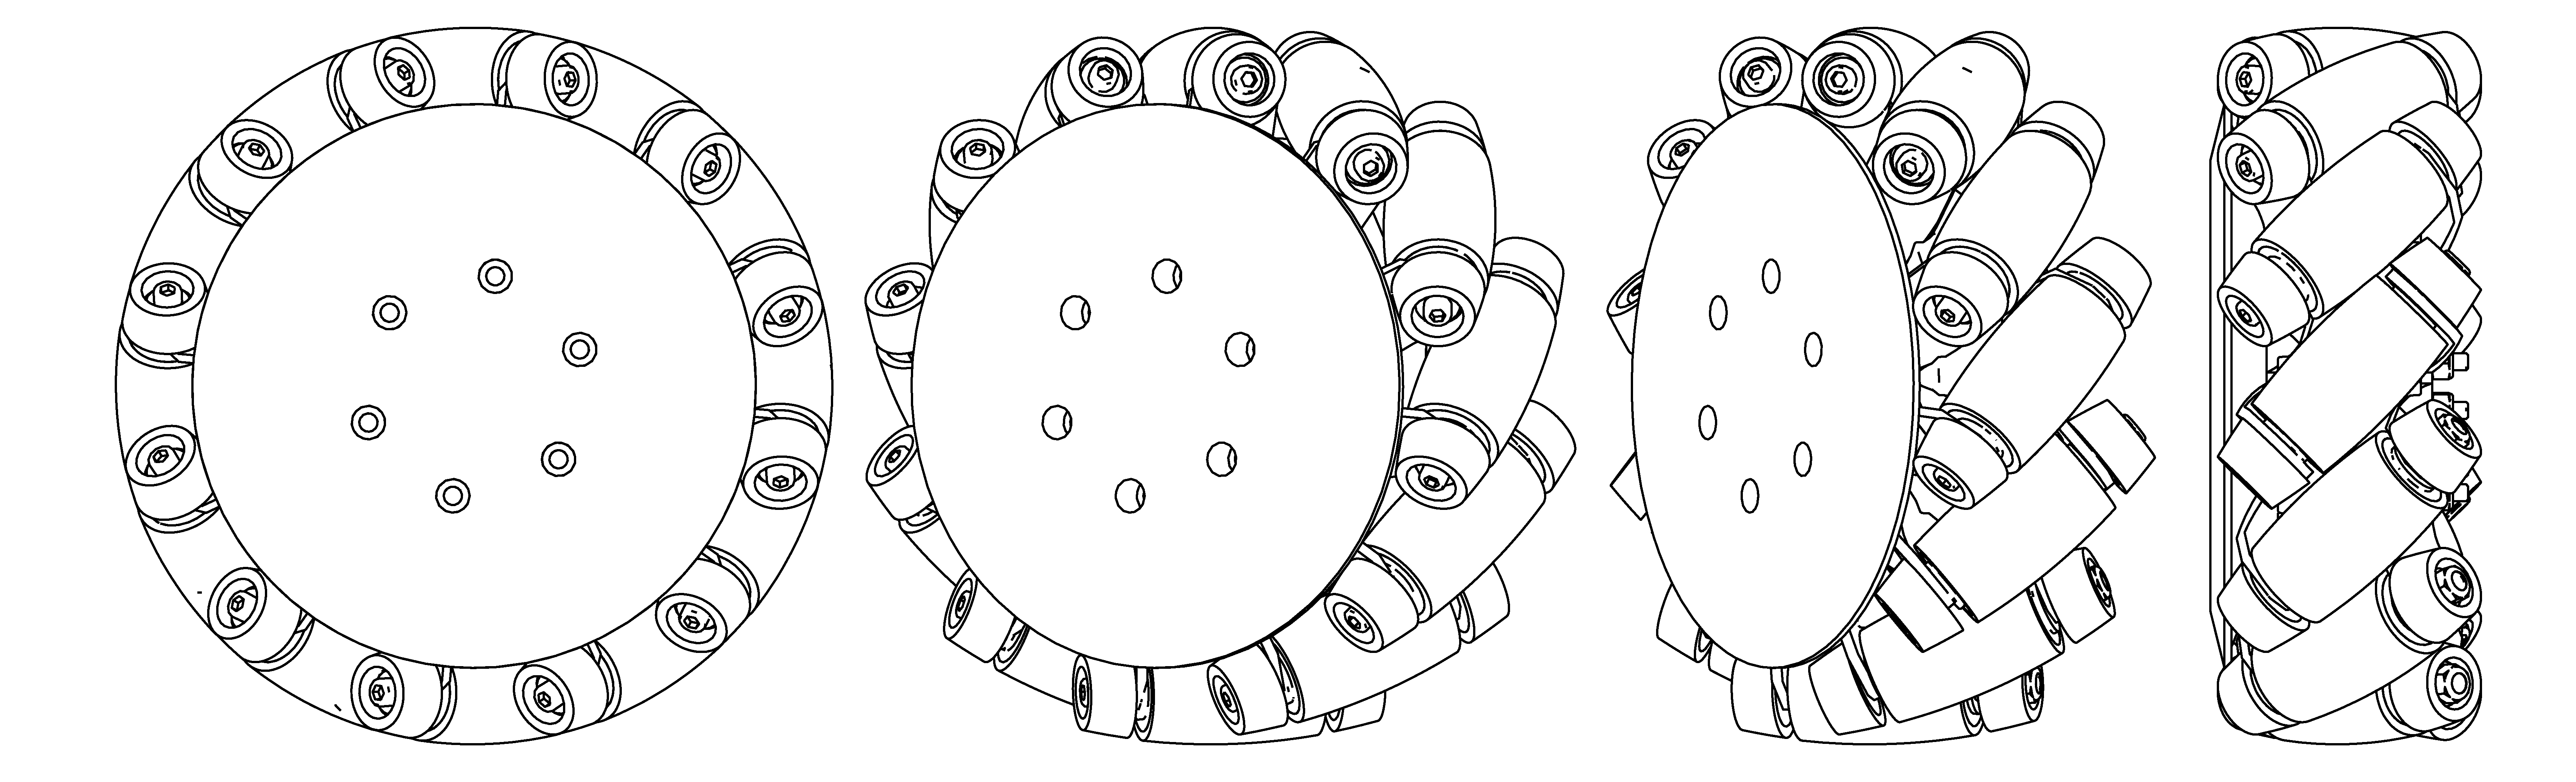
\includegraphics[width=\textwidth]{graphics/wheel.pdf}
	\caption{Widok 12 rolkowego koła szwedzkiego platformy wielokierunkowej.}
	\label{fig:wheel}
	\end{figure} 

	Każde koło ma 3 stopnie swobody \cite{kinematic_modeling}, tak samo jak cała platforma.
	\begin{itemize}
		\item Obrót koła w osi prostopadłej do płaszczyzny koła i przechodzącej przez jego środek.
		\item Rotacje pojedynczych rolek.
		\item Poślizg rolki w miejscu styku rolki z podłożem.
	\end{itemize}

	Na podstawie rysunku \ref{fig:wheel} można zauważyć, że krzywizna rolki jest tak ustawiona, aby punkt kontaktu rolki z podłożem w czasie obrotu koła płynnie przechodził na następną rolkę.
	Celem jest utrzymanie równej odległości osi obrotu koła od płaszczyzny podłoża.
	Nie powinno być efektu przeskoku z jednej rolki na drugą, gdyż to wprowadza nierówne tarcie, losowe poślizgi i nadmierne zużycie elementów wykonawczych.
	Kształt pojedynczej rolki jest wycinkiem paraboloidy, wzory opisujące kształt rolki są złożone.
	Zazwyczaj przybliża się taką rolkę wycinkiem torusa, w celu uproszczenia produkcji \cite{rollers}.

	Istnieją także koła o innej konstrukcji, złożone z wielu małych rolek, tak aby w każdym momencie więcej jak jedna rolka dotykała podłoża.
	Można także złożyć kilka powyższych kół obok siebie w jedno koło.
	Przydatne jest to dla robotów transportujących duże masy, gdyż zmniejsza to obciążenie pojedynczych rolek.
	Niestety, taka konstrukcja jest chroniona aktywnym patentem, więc pojedyncze koło, na które patent już wygasł, jest jedynym powszechnie używanym \cite{paletobot}.

	Podstawowym problemem konstrukcji koła jest nie tylko skomplikowana budowa, ale także ślizganie się rolek po powierzchni.
	Odległość osi obrotu koła od płaszczyzny podłoża nieznacznie zmienia się przy przenoszeniu ciężaru z rolki na rolkę, co przy dużych prędkościach powoduje drgania i jeszcze większe błędy szacowania pozycji

	\subsection{Ruch platformy na kołach}
		W zwykłym kole, dzięki tarciu, moment obrotu przekształcany jest na przyspieszenie w kierunku równoległym do podłoża i płaszczyzny koła.
		Dodatkowo wektory tarcia są równe we wszystkich kierunkach. To znaczy, koło będzie stawiało identyczny opór, niezależnie czy siła
		zostanie przyłożona wzdłuż osi obrotu koła, czy równolegle do płaszczyzny podłoża i płaszczyzny rolki.
		
		Specjalne koło Mecanum wywołuje tarcie kierunku obróconym o 45° w stosunku do osi obrotu koła, zależnie od typu koła (prawoskrętne lub lewoskrętne). 
		To oznacza, że przy nadaniu momentu siły $M$, wektor tarcia koła o powierzchnię $T$ będzie obrócony w stosunku do osi obrotu koła o 45°.
		Z kolei tarcie nada kołu siłę $F$ o przeciwnym zwrocie do wektora tarcia.
		Tarcie w kierunku $f_0$, prostopadłym do $F$, czyli zgodnie z obrotem najniżej położonej rolki, jest w idealnym przypadku zerowe.
		Z kolei wypadkowa siła od wszystkich kół nadaje platformie przyspieszenie i prędkość w odpowiednim kierunku.

		\begin{figure}[H]
		\centering
		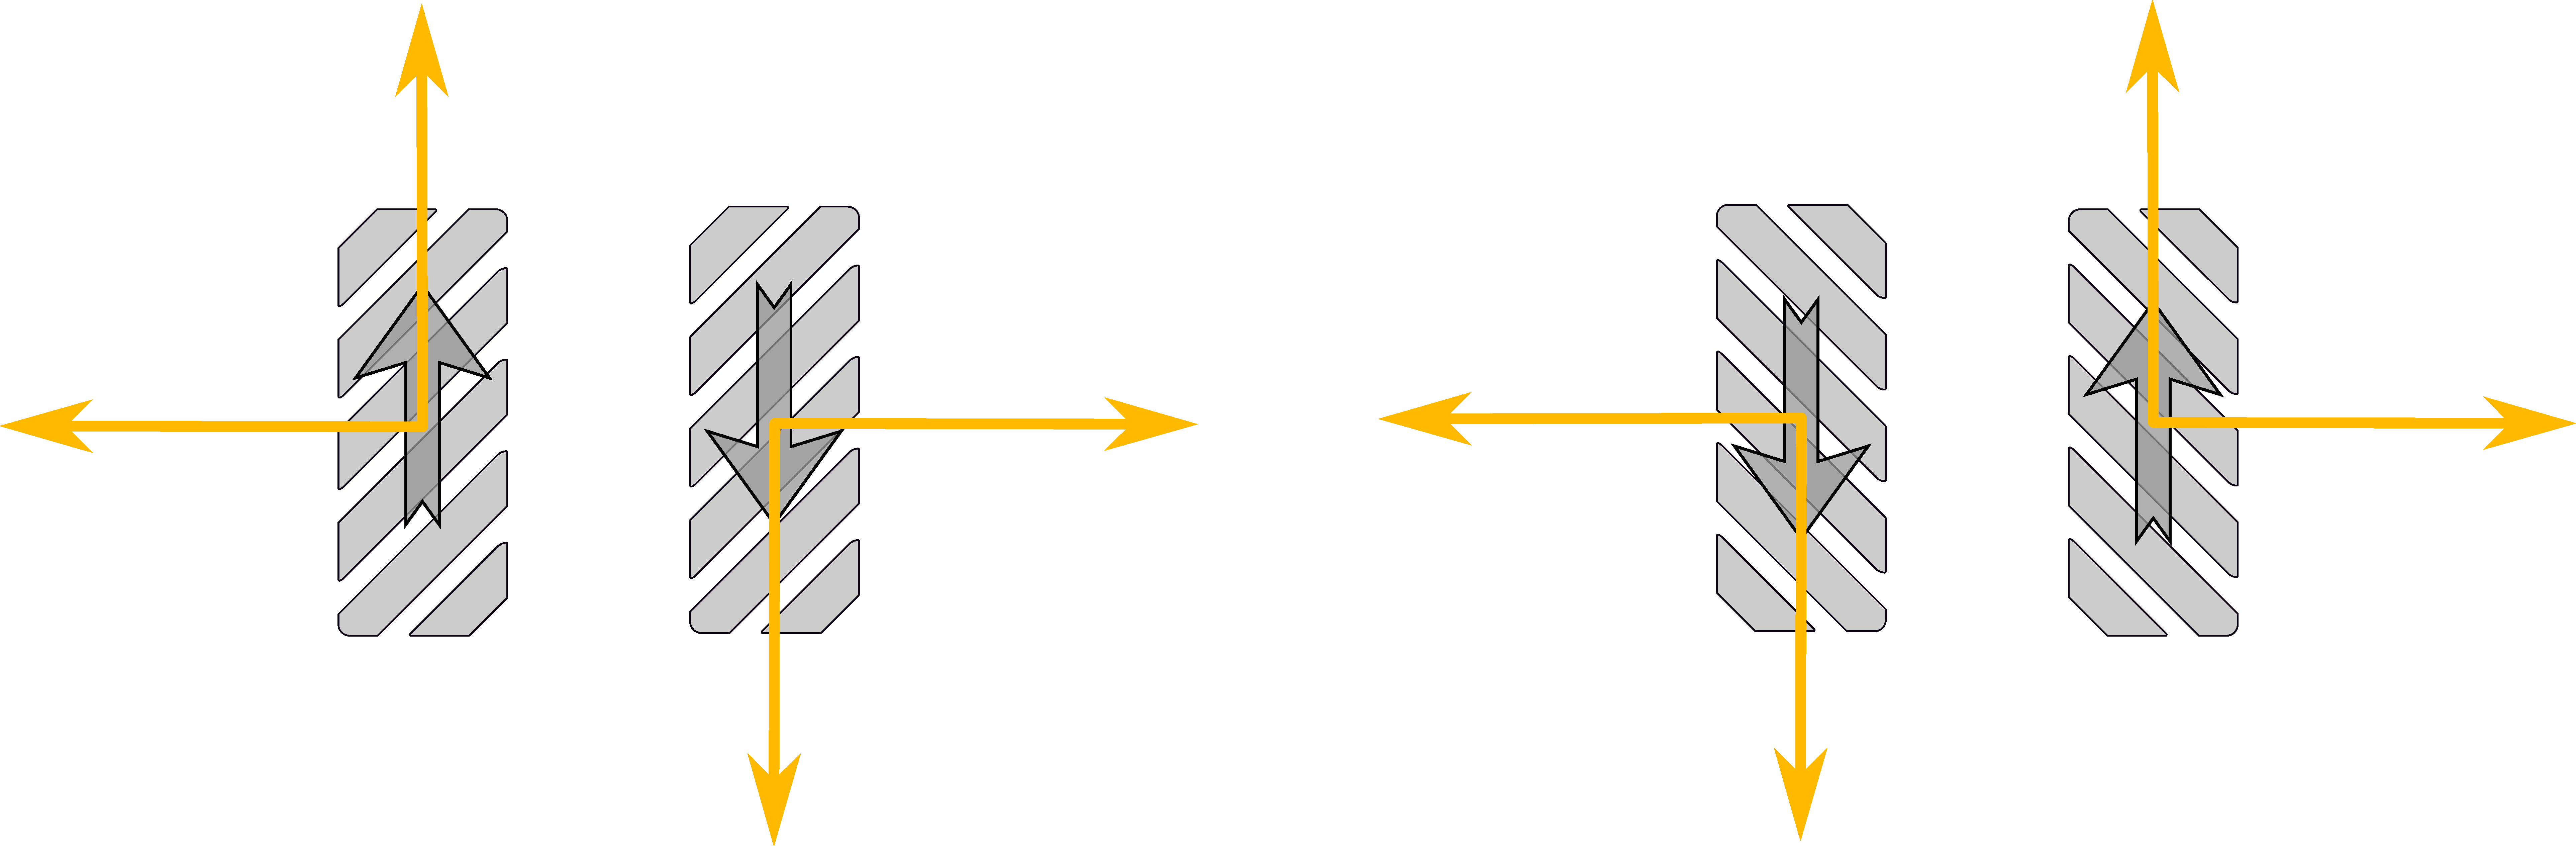
\includegraphics[width=\textwidth]{graphics/vectors.pdf}
		\caption{Wektory momentu siły i siły koła Mecanum, widzianego z góry.}
		\label{fig:wheel_vectors}
		\end{figure} 

		Ustawiając te koła w odpowiedni, pokazany na rysunku \ref{fig:base_dims}, sposób, można wywołać odpowiednie znoszenie się składowych sił,
		a w efekcie pozwolić robotowi na poruszanie się w kierunkach nieosiągalnych dla pojazdów o standardowych kołach.
		Warto nałożyć te wektory na wcześniejszy rysunek \ref{fig:mecanum_dirs}, aby dokładniej zobaczyć, 
		dlaczego koła nadają platformie daną prędkość wypadkową przy odpowiednim obrocie kół.

		\begin{figure}[H]
		\centering
		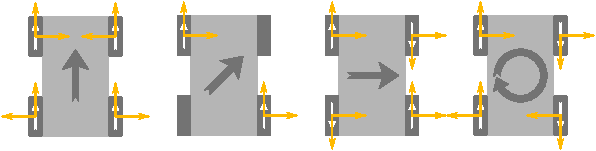
\includegraphics[width=\textwidth]{graphics/mecanum_dirs_vect.pdf}
		\caption{Ruchy platformy widzianej z góry, z nałożonymi składowymi wektorów sił.}
		\label{fig:mecanum_dirs_vect}
		\end{figure} 

		Warto rozpatrzyć każdy przypadek. Platforma posiada jedną płaszczyznę symetrii, ze względu na asymetryczny przegub.
		\begin{enumerate}
			\item Składowe wektorów sił o kierunku prostopadłym do pionowej płaszczyzny symetrii urządzenia znoszą się, ponieważ mają przeciwne zwroty na lewej i prawej parze kół.
			Pozostają jedynie składowe równoległe do płaszczyzny symetrii, które powodują prostoliniowy ruch naprzód.
			\item Dwa koła nie obracają się. Nie jest to ruch pasywny, gdyż taki wprowadzałby nieprzewidywane poślizgi, a aktywne hamowanie.
			Wektory się nie znoszą i platforma wykonuje ruch pod kątem 45° do płaszczyzny symetrii. Ruch odbywa się równolegle do kierunku $f_0$ zatrzymanych kół,
			zatem nie stawiają one w tym momencie oporu.
			\item Ruch podobny jest do przypadku 1. Tutaj również wektory znoszą się parami, jednak tym razem na przednich parach i tylnych. 
			Pozostają składowe prostopadłe do płaszczyzny symetrii, które nadają platformie przyspieszenie w bok.
			\item Prędkość kątowa powstaje, gdy wypadkowa kół po jednej stronie platformy znosi się z wypadkową po drugiej stronie.
		\end{enumerate}

		Warto nadmienić, że gdy wypadkowy wektor prędkości koła jest prostopadły do osi koła, to jest gdy
		koło porusza się zgodnie z kierunkiem obrotu, w idealnym przypadku rolki nie obracają się.
		Inaczej mówiąc, rolka będzie się obracać tym mocniej, im bardziej ruch koła wymuszany jest równolegle do osi koła, 
		czy to na skutek znoszenia się wektorów, czy oporu przeszkody.
		
		Przykładowo, przy ruchu naprzód, rolki koła się nie obracają, lecz przy ruchu w bok biorą aktywny udział.
		Ma to wpływ na zużywanie się tych elementów, nie tylko z punktu widzenia ilości obrotów danej rolki na pokonanym dystansie, 
		ale także sposobu w jaki wymuszany jest jej ruch.
		Rolki robota przy jeździe zawsze obracają się szarpanym ruchem w obie strony, ze względu na poślizgi od innych kół, 
		niejednostajne tarcie piast wszystkich rolek, czy różnice terenu. 
		Zatem przejazd przykładowego odcinka, przy platformie ustawionej przodem do kierunku jazdy, lub bokiem, będzie w różnym stopniu i w różny sposób zużywał elementy wykonawcze robota.
		To, jak dokładnie zużywają się przeguby i jaki styl jazdy opłaca się zastosować, aby zminimalizować uszkodzenia elementów jest dużą, odrębną dziedziną nauki.
		Odpowiednio skomplikowany algorytm sterowania może brać pod uwagę tą mechanikę kół.

\section{Enkodery}
	Każde koło posiada wbudowany w silnik enkoder. To urządzenie wykrywa aktualny ruch koła i zwraca jego aktualną prędkość i rotację.
	Korzystając z modelu kinematyki, można obliczyć z tych danych wypadkową prędkość robota, a następnie, za pomocą całkowania, wyznaczyć aktualną
	pozycję w stosunku do punktu startowego.
	
	W opisywanym robocie, silniki kół mają na tyle dużą moc, że wartość prędkości, wykrytej przez enkodery, bardzo niewiele odstaje od prędkości zadanej.
	Oznacza to, że teoretycznie, można nadawać kołom bardzo duże momenty sił, a koło rzeczywiście wykona zadaną akcję.
	Jednakże eksperymenty pokazały, że zasilacz robota może nie móc pracować przy takim poborze prądu i awaryjnie się odłączyć, co jest głównym powodem dla którego 
	należy ograniczać nadawanie zbyt dużych przyspieszeń platformie.

	Poślizg kół powoduje jednak, że odometria, bazująca na danych generowanych przez czujniki enkoderów, obarczona jest błędami losowymi i nie może być 
	użyta jako jedyna metoda wyznaczania pozycji względnej w trakcie jazdy robota \cite{heavy}. Zatem dodano do urządzenia także inne czujniki.
	
\section{Skaner laserowy}
	\label{sec:lidar}
	Dodatkowym czujnikiem, używanym przy wyznaczaniu pozycji platformy, jest skaner laserowy.
	Platforma wyposażona jest w dwa, dwuwymiarowe czujniki typu LiDAR firmy SICK.
	LiDAR to połączenie wyrazów \emph{light} i \emph{radar}, chociaż skrót może być rozwinięty w różne słowa.

	\begin{figure}[h]
	\centering
	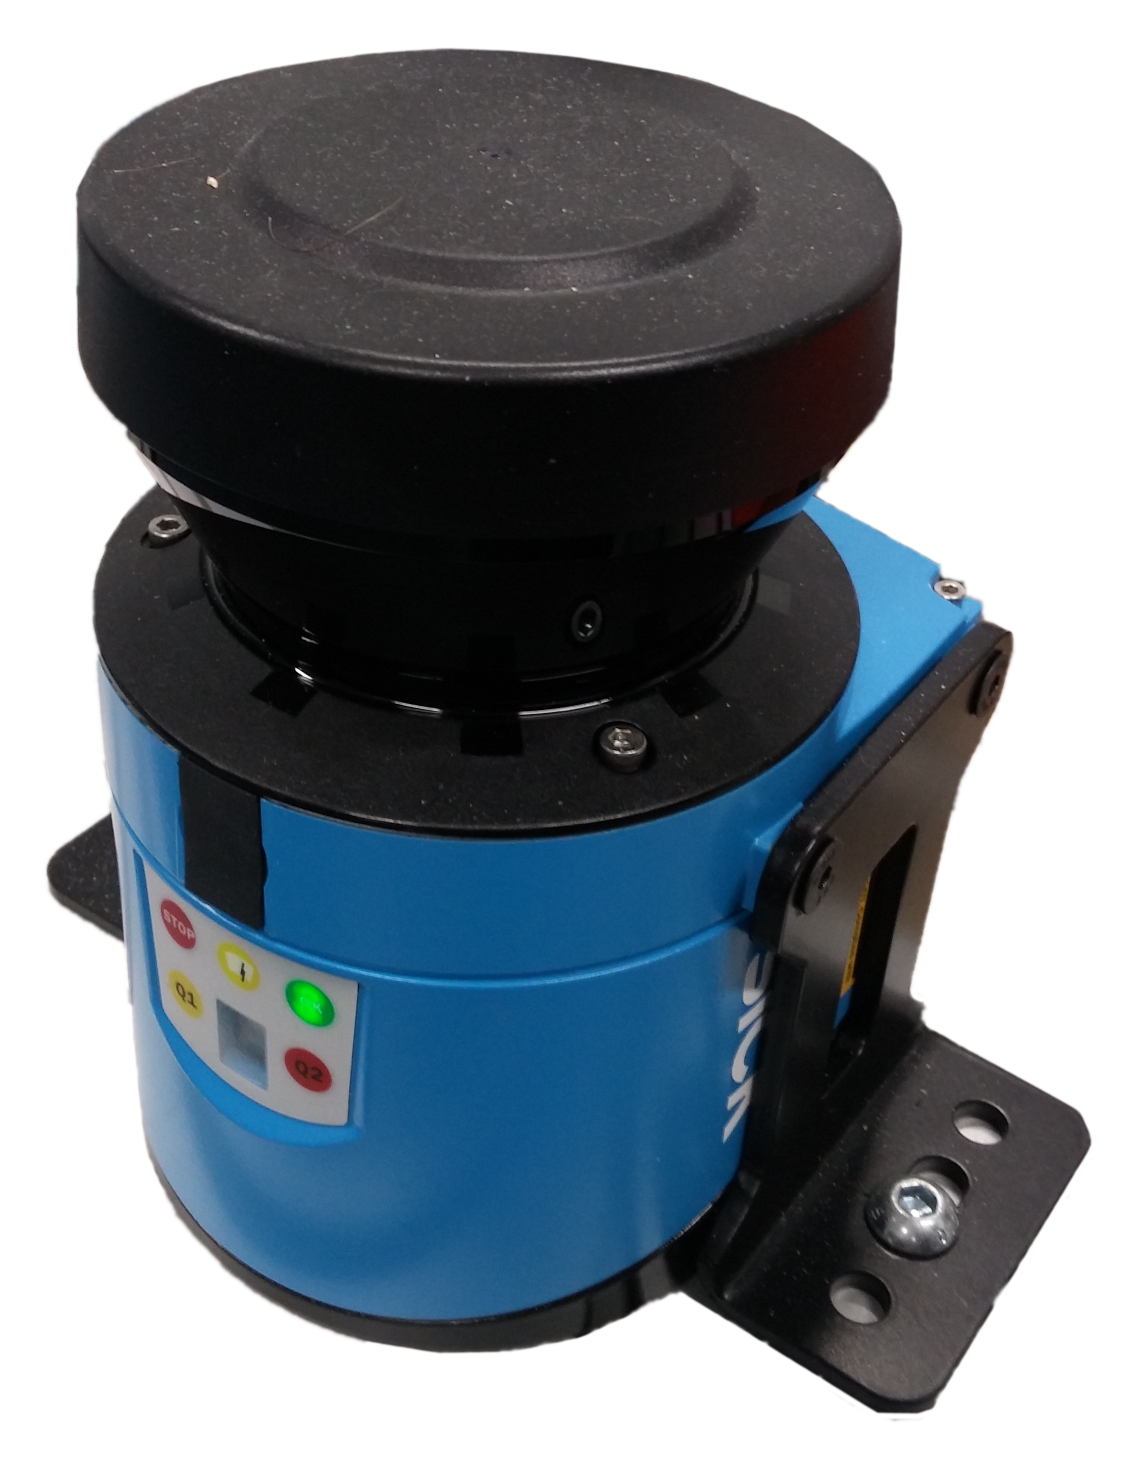
\includegraphics[width=0.5\textwidth]{graphics/sensor.png}
	\caption{Skaner laserowy SICK LMS100-10000.}
	\label{fig:sensor}
	\end{figure} 

	\subsection{Zasada działania}
		Wszystkie skanery tego typu mają bardzo podobną zasadę działania.
		W środku urządzenia znajduje się obrotowe lusterko, zwrócone pod kątem 45° do osi obrotu.
		Równolegle do osi jego obrotu znajduje się laser, który emituje pulsacyjną wiązkę podczerwonego promienia co pewien okres czasu.
		Emitowanie stałego promienia może być niebezpieczne dla wzroku obsługujących go ludzi.
		Aktualna pozycja lusterka jest wykrywana przez enkoder.
		Obok lasera jest czujnik, który bada wysłane przez laser, odbite od lusterka, obiektu i ponownie lusterka, światło.

		Na koniec, algorytm we wbudowanym mikrokontrolerze ustala kąt i odległość czujnika od wykrytego obiektu.
		Odpowiada także za usunięcie szumu i ewentualnych odbić promienia.
		Komunikacja z urządzeniem może odbywać się za pomocą różnych interfejsów sieciowych, zazwyczaj w architekturze typu master-slave.
		W przypadku tej platformy jest to Ethernet.
		
		Skośna szyba, będąca wycinkiem powierzchni stożka, zabezpiecza wnętrze przed zanieczyszczeniami, jej kształt niweluje ewentualne odbicia lasera, emitowanego poziomo ze środka.
		W niektórych czujnikach montuje się także szereg dodatkowych diod podczerwieni na obrębie szyby, skierowanych w górę, lub w dół, oraz czujniki/reflektory z drugiej strony.
		Pozwala to na wykrycie stopnia zanieczyszczenia szyby, aby powiadomić użytkownika o potrzebie wyczyszczenia urządzenia.

	\subsection{Komunikacja}
		Wysyłając do czujnika odpowiedni ciąg bajtów, można ustawić jego tryb działania, odpytać o zebrane dane, czy wykryć konfigurację i stan.

		W przypadku tej platformy, komunikacja odbywa się poprzez interfejsy EtherCAT i Ethernet.
		EtherCAT to sposób komunikacji urządzeń po kablu Ethernetowym, w trybie \emph{master}-\emph{slave}, przy zachowaniu sztywnych ram czasowych. 
		\emph{Master} wysyła pakiet do podłączonych szeregowo urządzeń \emph{slave}, które przekazują go przez siebie i w razie potrzeby modyfikują dane w locie.
		
		Program odbierający dane od czujnika komunikuje się bezpośrednio z urządzeniem, które zwraca pakiety zawierające pomiary z ostatniego obrotu czujnika, oraz dodatkowe dane 
		opisujące sam pomiar, takie jak czas, początkowy kąt pomiaru, czy tryb pracy.
		Dokładne pola w pakiecie i cechy czujnika dostępne są na stronie producenta \cite{sick_website}.

		Urządzenie wspiera uwierzytelnianie przez hasło, wgrywanie nowego oprogramowania,
		ustawienia czasu, oraz zmianę różnych parametrów działania.

	\subsection{Podstawowe cechy}
		Czujnik składa się z dwóch części, głównego trzonu, oraz nakładki.
		Połączenie tych elementów powoduje, że jego zakres pomiaru posiada martwy kąt.
		Przedstawia to dobrze grafika producenta \ref{fig:lidar}.
		\begin{figure}[h]
		\centering
		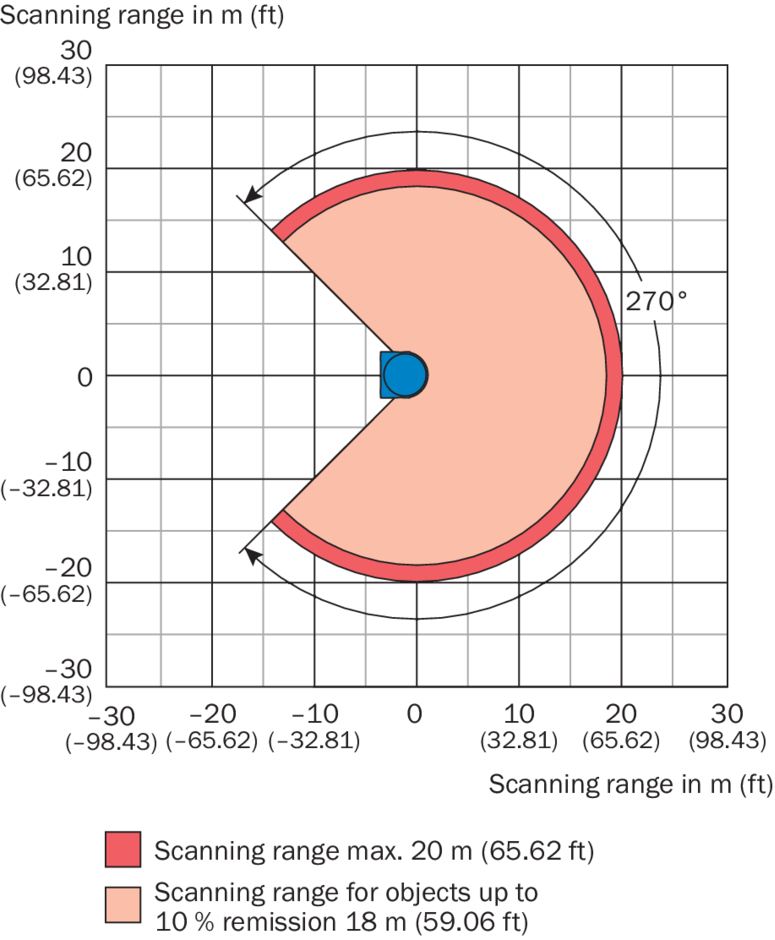
\includegraphics[width=0.6\textwidth]{graphics/sick.png}
		\caption{Wykres producenta dotyczący zasięgu czujnika \cite{sick_website}.}
		\label{fig:lidar}
		\end{figure} 
		
		\begin{table}
		\centering
		\begin{tabular}{l r}
		Cecha & Wartość \\
		\hline
		Kąt pracy & 270\textdegree \\
		Długość fali światła lasera & 905 nm (podczerwień) \\
		Częstotliwości skanowania & 25 Hz / 50 Hz \\
		Maksymalna odległość obiektu & $\approx$ 20 m \\
		Rozdzielczość kątowa & $0,25 \degree$ / $0,5 \degree $ \\
		Systematyczny błąd pomiarowy & $\pm 0,03$ m \\
		Przypadkowy błąd pomiaru odległości & $0,012$ m \\
		\end{tabular}
		\caption{Podstawowe cechy czujnika laserowego.}
		\label{tab:lidar}
		\end{table}
		Na podstawie tych danych można obliczyć, że w jednym przebiegu po całym zakresie kątowym urządzenia, 
		emitowane jest około 1080, lub 540 impulsów (w zależności od trybu działania).
		Taka liczba promieni wymagana jest w symulacji, aby wiernie odwzorować urządzenie.

\section{Jednostka inercyjna}
	Ten czujnik to małe urządzenie, posiadające zazwyczaj zestaw wewnętrznych czujników, przydatnych przy określaniu prędkości, rotacji i przyspieszeń modułu.
	Dodatkowo, wiele zestawów tego typu posiada także czujniki pola magnetycznego, położenia, lub nawet termometry.
	
	Czujnik użyty w platformie to ADIS16460AMLZ, firmy Analog Devices. Szczegółowa dokumentacja jest dostępna na stronie sprzedawcy \cite{adis_website}.
	
	Urządzenie ma kształt małej kostki i komunikuje się za pomocą złącza SPI, a co za tym idzie, wymaga zewnętrznego mikrokontrolera, aby móc wysyłać wygenerowane dane
	do sieci do innych urządzeń.
	
	Czujnik jest wyposażony w:
	\begin{itemize}
		\item Trzyosiowy żyroskop.
		\item Trzyosiowy akcelerometr.
		\item Czujnik temperatury.
		\item Sprzętowe wspomaganie korekcji błędów i kalibracji.
	\end{itemize}
	
	Błędy pomiarowe akcelerometra są bardzo duże, w stosunku do błędów pomiarowych żyroskopu i skanera laserowego. 
	Aby użyć tych danych w programie, należy zastosować na nich algorytmy usuwające szum i uśredniające wyniki.
	Rysując dane zebrane bezpośrednio z czujnika na wykresie, można jedynie z małą dokładnością określić kierunek przyspieszenia działającego na platformę, ale nie jego 
	wartość.
	
	W symulacji nie jest używana informacja o temperaturze otoczenia, zatem nie ma potrzeby jej symulować.
	
\section{Podłączenie urządzenia}
	Platforma podłączona jest do dedykowanego komputera, który pracuje z systemem operacyjnym Ubuntu i dodatkowymi modułami, które zapewniają 
	pracę w czasie rzeczywistym, aby urządzenie mogło poprawnie współpracować z robotem.
	
	Na tym systemie pracuje program, który przyjmuje komendy z innej sieci, odbierane z innego, biurowego komputera.
	Są tutaj także uruchomione algorytmy, obliczające pozycję platformy, bazując na odometrii.
	
\section{Sterowanie urządzeniami}
	Efektory robota wymagają podania odpowiedniego sterowania, a czujniki odpowiedniego odbiornika.
	\subsection{Sterownik silników}
		Program sterujący generuje abstrakcyjne dane, na przykład liczbę zmiennoprzecinkową, zapisaną binarnie.
		Przykładowy silnik fizyczny nie jest w stanie działać na podstawie takich danych, do pracy potrzebuje odpowiedniego napięcia na wejściu.
		Do tłumaczenia jednych danych na drugie, potrzebny jest sterownik niskopoziomowy.
		Najczęściej implementowany jest w formie mikrokontrolera, lub podobnego systemu wbudowanego.

		Jego zadanie to odczytanie danych, podanych przez program sterujący i na przykład generowanie na ich podstawie odpowiedniego przebiegu PWM, lub obsługa przetwornika cyfrowo-analogowego.
		Do innych zadań może należeć kontrola, czy żądana wartość nie uszkodzi urządzenia.
		Zazwyczaj sterownik może komunikować się z powrotem z resztą systemu, aby zgłaszać ewentualne awarie.

		Taki program i powiązany z nim układ elektroniczny są najczęściej dostarczone przez producenta robota i nieznane użytkownikowi.
		Dodatkowo, tworzy to kolejną warstwę abstrakcyjną dla sterownika głównego, który nie musi zważać na generowanie różnych danych dla różnych modeli tych samych efektorów.
		
	\subsection{Sterownik czujników}
		Implementowany podobnie do sterownika silników, ma za zadanie konwertować surowe i obarczone błędami dane z czujników na format zrozumiały dla programu sterującego.
		W tym miejscu usuwa się błędy grube, niweluje stałe na podstawie kalibracji, wygładza szum i interpretuje dane, aby pozyskać wymagane przez wyższe warstwy informacje.

		Przykładowo, czujnik zwraca jedynie ciąg pomiarów, ale to do tego programu należy połączenie pomiaru z informacją o emisji promienia, na ich podstawie obliczenie odległości od przedmiotu i porównanie z innymi pomiarami w celu usunięcia błędów grubych.
		Większość zaawansowanych receptorów posiada owe układy cyfrowe i programy wbudowane w urządzenie.
		Dostarczone są przez producenta tak samo, jak sterowniki efektorów.
		
		Aby zasymulować ten element, należy zbudować program generujący dane na podstawie aktualnego stanu maszyny do symulacji, w sposób w jaki działa czujnik w rzeczywistości.
		Na przykład, dla czujnika laserowego, silnik symulacji fizycznej emituje odpowiednią ilość promieni i oblicza ich punkty przecięcia się z wirtualnymi modelami.
		Renderowanie obrazu pozwala na symulację kamery.

		Ponieważ dane fizyczne nigdy nie są idealne, w celu przybliżenia wyjścia wirtualnego czujnika do oryginału, dodaje się szum o odpowiednim rozkładzie i błędy.

	\subsection{Program sterujący}
		W programie sterującym obliczane jest sterowanie, na podstawie dostarczonych odczytów z czujników.
		Zazwyczaj wykorzystuje się tutaj także zewnętrzne biblioteki, dostarczające zaawansowane algorytmy.
		Ich zadania mogą polegać na budowie wewnętrznej mapy, wyznaczaniu ścieżki, omijaniu przeszkód, odwrotnej kinematyce i tym podobnych.

		Taki program zwykle działa na mocniejszych układach logicznych, niż sterowniki, ze względu na duże zapotrzebowania na moc obliczeniową
		i niedeterministyczny czas obliczeń.
		Jeśli robot komunikuje się z użytkownikiem, to zachodzi to w tym module. 

		Programy sterujące mogą być implementowane w językach wysokopoziomowych, nawet skryptowych, gdyż wymagania czasowe nie są rygorystyczne.
		Co więcej, często się zdarza, że odpowiednie składowe programu bazują na różnych technologiach.

		Środowisko symulacyjne powinno zapewnić pełną abstrakcję komunikacji tego modułu.
		Oznacza to, że niezależnie, czy program steruje rzeczywistym robotem, czy symulacją wirtualną, zawsze powinien móc komunikować się i otrzymywać dane w tym samym formacie.
		W idealnym przypadku program nie powinien mieć możliwości stwierdzić, czy steruje symulacją, czy fizycznym urządzeniem.
		

\chapter{Środowiska programistyczne} 
\label{sec:tools}
W tym rozdziale opisane są narzędzia użyte do wykonania zadania.

Środowisko symulacji składa się z maszyny symulującej fizykę, odpowiedzialnej za obliczenia fizyczne, a także API do obsługi całej symulacji.
Zaawansowana maszyna symulacyjna powinna dobrze obsługiwać tarcia, więzy na ruch obiektów, przyłożone siły, materiały fizyczne dla określania tarcia i sprężystości obiektów, 
oraz wszystko to, co potrzebne do jak najwierniejszego odtworzenia zachowania rzeczywistego obiektu.

Na rynku jest wiele różnych maszyn, zarówno do symulacji w czasie rzeczywistym, jak i do wyznaczania pozycji obiektów po długich obliczeniach.
Istnieją technologie otwartoźródłowe, inne są własnościowe. Mogą używać tylko procesora, lub też być wspomagane przez kartę graficzną (na przykład \emph{PhysiX}).
Niektóre maszyny symulują, prócz zderzeń obiektów, także rozpływ cieczy, dymy, płótna, ciała sprężyste i strukturę wewnętrzną brył, 
lecz te funkcjonalności nie są potrzebne dla symulacji opisywanej platformy. Nazywa się je czasami ,,silnikami symulacji fizyki'', co jest bezpośrednim tłumaczeniem nazwy
\emph{physics engine} z języka angielskiego.

\section{\emph{Robot Operating System} (ROS)}
	Nazwa tego programu jest myląca.
	Nie jest to system operacyjny, lecz programowa struktura ramowa (\emph{framework}), zawierająca odpowiednie biblioteki i narzędzia do tworzenia programów sterujących \cite{ros_website}.
	Są tu algorytmy wyznaczania tras, budowy map, manipulowania robotycznymi ramionami, itp. 

	Programy w środowisku ROS pisze się w C++ lub Pythonie i integruje z robotem za pomocą kilku gotowych struktur kolejek wiadomości.
	Ta struktura ramowa zawiera także pakiety do wizualizacji odbieranych danych w formie graficznej.

	Działanie systemu jest oparte o pakiety.
	Każdy taki pakiet jest katalogiem zawierającym w sobie pliki opisujące jego parametry i skrypty CMake, używane do kompilacji.
	Pakiet może zawierać programy wykonywalne, dane, definicje, lub inne dowolne pliki.
	W symulacji opisywanej platformy, modele są pakietami, zawierającymi biblioteki ładowane dynamicznie, uruchamiane przez jeszcze inny pakiet symulatora.
	Pakiety mogą być zależne od siebie, osobno w kwestii kompilacji, jak i uruchomienia.
	
	ROS potrzebuje także działającego demona w tle. Odpowiada on za komunikację i kontroluje stany wszystkich węzłów.
	Z punktu widzenia konstrukcji systemu, można porównać go do jądra systemu operacyjnego, a węzły do działających procesów.
	Dlatego też nazwa \emph{Robot Operating System} nie jest przypadkowa.
		
	Na stronie internetowej ROSa, znajduje się bogata biblioteka pakietów, stworzonych przez inne osoby.
	Każdy może także umieścić tam swój własny pakiet, aby inni mogli go ściągnąć i wykorzystać w swoich projektach.

	Komunikacja pomiędzy programami odbywa się w sposób ciągły przez kolejki wiadomości, lub pojedyncze asynchroniczne wywołania, zwracające wynik.
	Program(węzeł) może nadawać strumień wiadomości do kanału komunikacyjnego, ale niekoniecznie musi istnieć w tym czasie odbiornik.
	Można buforować wiadomości, podglądać strumienie, tworzyć wykresy z danych, podłączać nadajnik do kilku odbiorników, podglądać graf komunikacji pomiędzy węzłami, itp.
	Do wszystkiego służy bogaty zestaw komend i wbudowanych narzędzi.
	
	Używane wbudowane narzędzia z tej struktury ramowej to:
	\begin{description}
		\item[\texttt{rosbag}] Narzędzie do zbierania i odtwarzania danych, wysyłanych przez kanał komunikacyjny.
		\item[\texttt{catkin}] System budujący pakiety, działający na skryptach CMake.
		\item[\texttt{roslaunch}] Program do wykonywania skryptu uruchamiającego pakiet.
		\item[\texttt{rosrun}] Program do uruchamiania pliku wykonywalnego z pakietu.
		\item[\texttt{rostopic}] Narzędzie do zarządzania węzłami, wysyłania i podglądania strumieni komunikacyjnych.
		\item[\texttt{roscore}] Demon ROS, zarządzający wszystkimi węzłami.
	\end{description}
	Dodatkowo, używane funkcjonalności funkcji bibliotecznych:
	\begin{itemize}
		\item Rejestracja nowego węzła w demonie ROS.
		\item Stworzenie nadajnika strumienia wiadomości.
		\item Stworzenie odbiornika strumienia wiadomości.
		\item Powiadomienia.
		\item Nadawanie macierzy przekształceń jednorodnych.
		\item Zawieszenie programu.
	\end{itemize}


\section{Gazebo}
	Gazebo \cite{gazebo_website} jest symulatorem graficznym, działającym na podstawie uprzednio przygotowanych plików konfiguracyjnych.
	Zazwyczaj używany w trybie wsadowym, uruchamiany z argumentami z linii poleceń i plikiem opisującym symulację.
	Plik ten zawiera nazwy i ścieżki umieszczanych w symulacji modeli i wtyczek.
	Z tego powodu interfejs graficzny jest dość ubogi.

	Program wykonuje symulację z wykorzystaniem podanych modeli, używając jednego z czterech popularnych maszyn symulacyjnych: ODE, Bullet, Simbody lub DART.
	Wszystkie te symulatory są wolnym oprogramowaniem i używane są także w innych programach, na przykład w edytorze Blender.

	Symulator oprócz tego ma wbudowany edytor modeli, w którym można składać i ustawiać odpowiednie obiekty razem w przestrzeni trójwymiarowej
	i generować plik opisujący symulację.
	Edytor budynków pozwala na stawianie wirtualnych ścian, korytarzy, drzwi i ogólnego otoczenia, w którym roboty mogą pracować i być symulowane.
	Funkcjonalność tych edytorów jest bardzo ograniczona, brak jest tak podstawowych funkcji, jak cofanie ruchu.
	Dlatego lepiej jest zdefiniować model w pliku tekstowym.
	Również tworząc modele poza edytorem, posiada się nad nimi większą kontrolę, a parametry składowych da się ustawiać z dowolną dokładnością.

	Gazebo przyjmuje modele w specjalnym formacie SDF. Jest to standaryzowany, zdefiniowany niezależnie od symulatora format, do opisywania budowy robotów i czujników.
	Dzięki temu plik SDF może być użyty w innej symulacji, w innym programie, pod warunkiem przestrzegania standardu.
	Składnia jest zgodna ze standardowym językiem XML, co znaczy, że może być tworzona na dowolnym edytorze tekstowym.

	Wtyczka do sterowania modelem jest skompilowaną biblioteką, dołączaną na starcie programu.
	Tworzy się ją w C++ lub Pythonie, jako klasę dziedziczącą po abstrakcyjnej klasie dostarczonej przez Gazebo.
	Dzięki temu może korzystać ze wszystkich funkcji systemu operacyjnego, jak na przykład komunikacja za pomocą pamięci współdzielonej.
	Gazebo dostarcza także swój własny mechanizm kolejek wiadomości, który sprawdza się w jednolitej komunikacji z zewnętrznymi programami, korzystającymi z symulatora Gazebo, jednak jest niezależny od podobnej mechaniki ROSa. Z punktu widzenia ROSa, programy uruchamiane w Gazebo są jednym węzłem, który posiada wiele strumieni komunikacyjnych,
	zarówno dostarczonych przez sam symulator, jak i wczytanych wtyczek.

	Program jest w pełni wspierany na dystrybucji GNU/Linuksa Ubuntu ale bez problemu można go także skompilować na innych dystrybucjach.
	Nie wspiera innych systemów operacyjnych.
	Interfejs jest dopracowany i przestrzega systemowych ustawień DPI, lecz nie korzysta z dedykowanych bibliotek do tworzenia 
	interfejsów typu Qt, lub GTK.
	Uruchamianie programu jest proste i nie wymaga dodatkowych ustawień, wywoływania skryptów inicjalizujących, 
	tworzenia odpowiednich katalogów, czy definiowania zmiennych systemowych.
	Podobnie jak inne programy, tworzy ukryty katalog w katalogu domowym użytkownika, gdzie składuje wszystkie modele i logi.

	Gazebo może także być składnikiem systemu ROS, kod źródłowy jest dzielony w ramach wspólnej organizacji.
	Kolejne wersje Gazebo są powiązane z kolejnymi wersjami ROSa, nie można użyć przestarzałej wersji Gazebo z nowszym ROSem i odwrotnie.
	Symulator można zainstalować osobno lub jako jeden z pakietów ROSa.
	Jednakże, ze względu na chęć zachowania wysokiej kompatybilności pakietów ROSa, nie zawsze najnowsza wersja symulatora jest dostarczana razem z najnowszą wersją programowalnej struktury ramowej.
	
	Gazebo implementuje prawie wszystkie elementy standardu SDF, ale tylko niektóre będą używane. Posiada także kilka narzędzi do wizualizacji wygenerowanych danych, ale i ROS je posiada.
	\begin{itemize}
		\item Symulacja fizyki za pomocą maszyny do symulacji ODE.
		\item Całkowanie prędkości poprzez umieszczenie obiektu kinematycznego w przestrzeni wirtualnej i nadawanie mu prędkości.
		\item Możliwość modyfikacji wektorów tarcia.
		\item Dane o prędkościach i pozycjach wszystkich obiektów na scenie.
		\item Symulacja skanera laserowego.
		\item Symulacja jednostki inercyjnej.
		\item Wizualizacja obiektów za pomocą siatki trójkątów i kolorów.
		\item Wizualizacja kolizji, kształtów i inercji obiektów.
		\item Wizualizacja pozycji i rotacji poszczególnych obiektów, ich lokalne układy współrzędnych.
	\end{itemize}

\section{V-Rep}
	V-Rep \cite{vrep_website}, to duże i złożone środowisko, reklamujące się wieloma zaawansowanymi mechanizmami i funkcjami.
	Pomimo otwartego kodu, użycie komercyjne jest płatne. Dla zastosowań akademickich program jest bezpłatny.
	Bogaty interfejs graficzny zakłada budowę i symulację wszystkiego w tym jednym programie.

	W środowisku używa się dwóch z maszyn symulacyjnych, wykorzystywanych w Gazebo, czyli ODE i Bullet, oraz dodatkowo Vortex i Newton. Z tej czwórki tylko Vortex ma zamknięty kod.

	Głównym mankamentem programu jest zapisywanie utworzonych w systemie modeli.
	Program tworzy drzewiastą strukturę modelu, w pliku binarnym własnego formatu, co uniemożliwia edycję i wizualizację modelu bez uruchamiania całego programu 
	i importowania modelu do symulacji.
	Brak przenośności, czy wsparcia systemu kontroli wersji dla takich nietekstowych plików także jest problemem.

	Pisanie wtyczek najczęściej odbywa się w języku Lua. Poprzez komunikację sieciową, są też też dostępne inne języki, jak C, Matlab, Java, itp.
	Komunikacja z innymi programami odbywa się poprzez specjalne wtyczki do środowiska.
	API pozwala stworzyć mały, wbudowany interfejs graficzny do sterowania symulacją poprzez przyciski i suwaki.

	Ze strony producenta pobrać można gotowe archiwum z programem, który nie wymaga żadnej instalacji i posiada wszystkie potrzebne zasoby do pracy i nauki, 
	jak przykładowe modele istniejących komercyjnych robotów.
	Program działa w trzech najpopularniejszych systemach operacyjnych --- Windows, Linux i OS X.
	
	Przy wykonywaniu zadania, użyty będzie jeden z gotowych modeli robotów wielokierunkowych, wspomniana wcześniej Kuka Youbot, aby na jego podstawie zbudować model opisywanej platformy. Zostanie zapisany skrypt w Lua, który będzie używał wbudowanych mechanik do komunikacji ze strukturą ramową ROS. 
	Symulator ODE, ten sam co w Gazebo, będzie zastosowany w symulacji, ponieważ daje najlepsze wyniki. Interfejs graficzny do sterowania robotem nie będzie używany.

\section{Pozostałe narzędzia}
	Do tworzenia oprogramowania na systemach Unixowych można użyć dowolnych edytorów, gdyż standardowo wszystko jest potem kompilowane za pomocą narzędzi wiersza poleceń i skryptów.
	Jednak warto sobie ułatwić pracę zaawansowanymi środowiskami graficznymi.
	\begin{description}
	\item[CMake] to popularny i używany przez ROS i Gazebo system budowy kodu. Program tworzy na podstawie swoich plików konfiguracyjnych plik \texttt{makefile} do kompilacji źródeł i łączenia bibliotek.
	\item[GCC] będzie użyty do kompilacji, gdyż jest to najpopularniejszy tego typu program używany w GNU/Linux. Same symulatory zostały w nim skompilowane.
	\item[KDevelop] jest graficznym edytorem tekstowym i nadaje się do pisania kompilowalnego kodu wtyczek. Można podłączyć je pod komendę \texttt{make} i korzystać z mechanizmów interpretacji błędnych linii kodu, graficznego debugowania i podobnych.
	\item[Bash] będący bardzo popularnym językiem skryptowym nadaje się do automatyzacji pracy i uruchamiania testów w kontrolowany i prosty sposób.
	Uniwersalne narzędzie pomagające w wielu miejscach.
	\item[Git] jest narzędziem kontroli wersji, używanym przy bardzo wielu projektach informatycznych. Pozwala na łatwe umieszczenie kodu w repozytorium GitHub.
	\item[Gnuplot] służy do generowania wykresów z danych, zapisanych w pliku tekstowym.
	\item[Dia] to graficzny edytor do tworzenia diagramów UML.
	\end{description}



\chapter{Model platformy}
Pierwszym krokiem do stworzenia modelu dynamicznego, jest stworzenie modelu kinematycznego, aby móc porównać z nim tworzony model dynamiczny, oraz fizyczną platformę,
w celu weryfikacji poprawności działania.
Dzięki temu można łatwo oszacować, jak bardzo błędy symulacji, oraz błędy niedoskonałości fizycznego modelu odstają od matematycznych wyliczeń.

Dodatkowo, stworzenie modelu platformy kinematycznej pozwala na proste odrzucanie niedziałających implementacji modelu kinematycznego.
Model platformy kinematycznej ma także kluczowe zastosowanie w odometrii.

\begin{figure}[H]
\centering
 \includegraphics[width=0.8\textwidth]{graphics/base_dims.pdf}
\caption{Wielkości używane we wzorach.}
\label{fig:base_dims}
\end{figure} 

\begin{table}
\centering
\begin{tabular}{c c l}
Oznaczenie & Wartość & Opis \\
\hline
$r$ & 0,1 m & Promień koła w najszerszym miejscu na środku. \\
$a$ & 0,76 m & Szerokość platformy między środkami kół tej samej osi. \\
$b$ & 0,72 m & Długość platformy między środkami kół tego samego boku. \\
$\omega_i$ & & Prędkość kątowa każdego z kół. \\
$v_x$ & & Prędkość transwersalna w osi X. \\
$v_y$ & & Prędkość transwersalna w osi Y. \\
$\omega_z$ & & Prędkość kątowa w osi Z, wektor skierowany w górę. \\
\end{tabular}
\caption{Opisy i wartości symboli używanych we wzorach i rysunkach.}
\label{tab:dims}
\end{table}

\section{Sposób zapisu w formacie SDF}
\label{sec:sdf}
	\emph{Simulation Description Format} (SDF) jest formatem XML, pozwalającym na określenie elementów i zależności pomiędzy nimi w przestrzeni trójwymiarowej, 
	w szczególności budowy i rozmieszczenia robotów.
	Powstał jako zamiennik poprzedniego formatu URDF ze względu na jego skomplikowaną semantykę i brak możliwości określania środowiska wokół robotów, 
	na przykład rozmieszczenie elementów na symulowanej scenie, określania wyglądu i fizycznego zachowania się materiałów itp.

	W przeciwieństwie do poprzednika zapisującego model w przestrzeni drzewiastej, SDF równolegle określa wszystkie składowe modelu, 
	oraz zależności między nimi, jak więzy i względne pozycje.
	Model składowych robota ma strukturę gwiazdową. Jeden element, \texttt{model}, jest nadrzędny, wszystkie składowe są logicznie rozmieszczone równolegle.
	Specjalnie opisane więzy definiują interakcje pomiędzy elementami.
	Jako model, standard rozumie nie tylko roboty, ale także obiekty typu przeszkody, źródła światła, elementy animowane i tym podobne.
	Standard jest dobrze opisany na ich stronie internetowej \cite{sdf_website}.

	Element typu \texttt{world}, równoległy do modeli, zawiera informacje o środowisku symulacji.
	Dodatkowo można dodać informację o ustawieniach maszyny symulującej fizykę, wyglądzie sceny, wietrze, grawitacji, polu magnetycznym itp.

	W każdym z modeli, zawiera się nazwa, domyślna pozycja, sposób traktowania przez symulator i wtyczki programów obsługujących zaawansowane zachowanie modelu,
	opisane w równoległych do składowych elementach, ale jako że wszystkie te mogą wystąpić tylko raz, należy traktować je jako część elementu \texttt{model}.
	Model, lub jego fragment, może być zaimportowany z innego pliku, lecz nie zmieni to struktury gwiazdowej, a co za tym idzie, może dojść do utraty informacji.
	Ten przypadek zachodzi przy modelach czujników laserowych, opisanych w rozdziale \ref{sec:monokl}.

	Model zawiera w sobie równolegle wszystkie elementy typu \texttt{link}, każdy z nich jest osobną, kompletną częścią robota, na przykład kołem, 
	fragmentem ramienia chwytaka, kadłubem, czujnikiem.
	Składowa w sobie informacje o pozycji względem lokalnego środka układu współrzędnych modelu, masie, kształcie, fizycznym kształcie, materiale fizycznym i wyglądzie.
	Pozwala na dodanie elementów reprezentujących źródła dźwięku, czujniki, baterie itp.

	Same elementy zawierają jedynie informacje o swoim początkowym umiejscowieniu w modelu, ale nie o sposobie poruszania się i nałożonych więzach.
	Do tego potrzebne są, równoległe do elementów modelu, typy \texttt{joint} określające typ więzów, osie, współczynniki sprężystości, wytrzymałość, siłę silników.
	Każde połączenie określa, między jakimi obiektami się łączy.
	
	\begin{figure}[H]
	\dirtree{%
	.1 sdf.
	.2 world\DTcomment{Opis przestrzeni symulacji}.
	.2 model\DTcomment{Model w przestrzeni}.
	.3 plugin\DTcomment{Program sterujący modelem}.
	.3 link\DTcomment{Składowa modelu}.
	.4 collision\DTcomment{Fizyczny kształt składowej}.
	.4 visual\DTcomment{Siatka definiująca wygląd składowej}.
	.4 sensor\DTcomment{Czujnik w składowej}.
	.5 plugin\DTcomment{Program sterujący czujnikiem}.
	.3 joint\DTcomment{Wiąz pomiędzy składowymi}.
	}
	\caption{Najważniejsze elementy formatu SDF.}
	\label{fig:sdf_dir}
	\end{figure} 
	
\section{Model kinematyczny}
	\label{sec:pseudovelma}
	Kinematyka to nauka o ruchach obiektów na podstawie nadanych wektorów prędkości.
	Pomija ona takie aspekty jak masa, moment bezwładności, czy siły.
	
	Model kinematyczny jest sterowany funkcjami matematycznymi, 
	zamieniającymi prędkość kątową kół platformy na prędkości transwersalne geometrycznego środka platformy w układzie współrzędnych lokalnych, oraz jego prędkość kątową. 
	Symulator pozwala również na całkowanie tego ruchu, aby uzyskać aktualną pozycję platformy.
	
	Funkcje tłumaczące prędkości kół najwygodniej zapisać w postaci macierzowej, podobnie do tego, jak opisano w \cite{wheels}. 
	Wzór powtarza się w wielu innych pracach naukowych, a jego dokładny kształt zależy od kolejności numerowania kół i interpretacji wymiarów.
	Dla opisanego tutaj przypadku, (stałe zdefiniowane są w tabeli \ref{tab:dims}):
	
	\begin{equation}
	\begin{bmatrix}
	v_x \\
	v_y \\
	\omega_z \\
	\end{bmatrix}
	=
	\frac{r}{4}
	\begin{bmatrix}
	-1 & 1 & -1 & 1 \\
	1 & 1 & 1 & 1 \\
	\frac{2}{a+b} & \frac{-2}{a+b} & \frac{-2}{a+b} & \frac{2}{a+b} \\
	\end{bmatrix}
	\begin{bmatrix}
	\omega_1 \\
	\omega_2 \\
	\omega_3 \\
	\omega_4 \\
	\end{bmatrix}
	\end{equation}
	
	Uzyskane wartości należy przemnożyć przez odpowiednie wektory jednostkowe, obrócić względem lokalnego układu współrzędnych dla modelu i zastosować w funkcjach nadających prędkości bryle.

	Ponieważ sterowanie pozycją modelu kinematycznego odbywa się wyłącznie poprzez wzory matematyczne, w jego symulacji nie uczestniczy maszyna symulacyjna fizyki.
	Taki model nie reaguje na kolizje z innymi obiektami, nie reaguje na różnicę terenu i nie używa informacji o współczynnikach tarcia materiałów, jak model dynamiczny.

	Nazwa kodowa \texttt{pseudovelma} odnosi się do tego, że jest to nieprawdziwy ruch sterowany z zewnątrz, a nie prawdziwa symulacja.

	\subsection{Problemy implementacji}
		Gazebo nie ma zaimplementowanego pełnego wsparcia dla standardu SDF.
		W szczególności nie działa struktura elementów \texttt{frame}, odpowiadająca za transformacje obiektów względem innych obiektów.
		Nie jest to zapisane w dokumentacji, a jedynie zgłoszone od kilku lat w systemie kontroli wersji jako błędy.

		Oznacza to, że wszystkie elementy typu \texttt{link}, będąc dziećmi \texttt{model}, nie zachowują swojej pozycji w lokalnym układzie współrzędnych.
		Powoduje to, że nadając prędkość kątową modelowi za pomocą funkcji, nadajemy ją każdej składowej osobno.
		Każde z kół i dwie części bazy, obracają się zgodnie z zadanymi wartościami, ale ich środki pozostają w miejscu w którym rozpoczęły symulację,
		ignorując kompletnie pozycję zdefiniowaną dla elementu rodzica \texttt{model}.
		
		Z punktu widzenia symulacji fizycznej ma to sens, gdyż nie można zakładać że składowe modelu są w jakikolwiek sposób podłączone do jego głównej części
		(która wcale nie musi mieć zdefiniowanego kształtu fizycznego), to wprowadzałoby także nieścisłości w typie połączenia, niektóre elementy powinny być przecież ruchome.

		Aby przeciwdziałać temu zjawisku, należy przenieść zawartość elementów \texttt{link} do elementu \texttt{model} i ustawić je jako \texttt{visual} elementu \texttt{model}.
		W ten sposób traktowane są jako część renderowana modelu, a nie osobne składowe.
		Nie można użyć tutaj więzów statycznych, gdyż te są wykorzystywane przez maszynę symulacyjną fizyki i ignorowane są przy kinematycznym ruchu.

		Powstała niedogodność jest taka, że ciężej jest sterować obrotem elementów \texttt{visual}, gdyż są zarządzane przez kompletnie inny system symulatora,
		służący do graficznego renderowania sceny.
		Oczywiście ma to znaczenie jedynie kosmetyczne, gdyż w żaden sposób nie wpływa na ruch modelu bazy.

	\subsection{Komunikacja}
		Komunikacja programu sterującego platformą odbywa się przez wbudowane z ROSa narzędzie \emph{topic}.

		Wiadomość zawierająca dane prędkości kół czterokołowego robota nie mieści się w standardzie, zatem został stworzony specjalny typ \texttt{omnivelma\_msgs/Vels}.
		Ta stryktura zawiera cztery wartości zmiennoprzecinkowe podwójnej precyzji, oznaczające prędkości w rad/s.

		Program w każdym cyklu symulacji nadaje wiadomości:
		\begin{itemize}
		\item \texttt{geometry\_msgs/PoseStamped} z aktualną pozycją i rotacją platformy, oraz nagłówkiem z identyfikatorem i czasem nadania pakietu.
		\item \texttt{geometry\_msgs/TwistStamped} z aktualną prędkością platformy, oraz identycznym nagłówkiem.
		\item \texttt{nav\_msgs/Odometry} z obiema powyższymi danymi i nagłówkiem. Służy przy obliczaniu ruchów platformy na podstawie enkoderów kół.
		\end{itemize}
		Ponadto program przyjmuje dane:
		\begin{itemize}
		\item \texttt{omnivelma\_msgs/Vels} z zadanymi prędkościami kół.
		\end{itemize}

	\subsection{Zachowanie}
		Platforma ignoruje kompletnie otoczenie, poruszając się przez inne obiekty na scenie.
		Po nadaniu stałych prędkości kół, następuje ruch po okręgach zgodnie z rysunkiem \ref{fig:mecanum_dirs}.

		Program sterujący, co każdą klatkę symulacji (okres zależy od zasobów procesorowych komputera), zwraca aktualną pozycję i rotację, 
		działając jak układ całkujący funkcje ruchu z powyższej macierzy.

\section{Model dynamiczny}
	\label{sec:omnivelma}
	Wykorzystując maszynę do symulacji fizyki, można umieścić w niej model określający kształty, masy i zależności pomiędzy składowymi modelu, 
	następnie nadać elementom wirtualne siły i otrzymać przybliżone wyniki do tego, jak zachowywałaby się rzeczywista platforma.

	Wszystkie programy i definicje związane z tym modelem noszą nazwę \texttt{omnivelma}, co nawiązuje do wielokierunkowości ruchów robota manipulującego, którego podstawa ma transportować.

	Robot jest bryłą, na którą składają się następujące części składowe:
	\begin{itemize}
	\item Główna część trzonu.
	\item Ruchoma, mniejsza część trzonu z przodu robota.
	\item 4 koła, 2 podłączone do głównej części, a 2 do przedniej.
	\item Po 12 rolek na każdym kole.
	\item Przegub zawiasowy, łączący dwie części podstawy.
	\item 4 przeguby zawiasowe z silnikami, łączące części bazy z kołami.
	\item 12 przegubów zawiasowych na każdym kole, łączących koła z rolkami.
	\end{itemize}

	Jest to dość skomplikowany obiekt do symulacji, dlatego należy skłonić się do znalezienia sposobu na uproszczenie modelu, w celu zmniejszenia ilości obliczeń symulatora
	i błędów reprezentacji liczb zmiennoprzecinkowych.

	Istnieje wiele podejść do stworzenia odpowiedniego modelu. Każde z nich było proponowane na różnych forach przez osoby symulujące podobne bazy, a także w zawartej bibliografii.
	
	Jednak idealne rozwiązanie nigdy nie zostało znalezione.
	Działający w tym przypadku sposób, także nie został wcześniej sprawdzony.

	\subsection{Jak największe zbliżenie do oryginału}
		Wspomniany wyżej sposób jest najbardziej wymagającym obliczeniowo, ale także najprostszym z możliwych.
		Należy stworzyć elementy składowe systemu i nadać im fizyczny kształt za pomocą odpowiedniej siatki trójkątów.
		Kształt obiektów może być także ustalony jednym prymitywów, jak sześcian, kula, łamana, walec i płaszczyzna.
		Takie przybliżenie znacznie przyspiesza obliczenia, gdyż może być specjalnie traktowane przez algorytmy.

		Słabym punktem tego rozwiązania jest fakt, że rolki są niestandardowym kształtem, opisanym dokładniej w \cite{rollers}, 
		którego dokładność jest bardzo wysoce wymagana dla zmniejszenia niedokładności ruchów.
		Przybliżenie jej walcem powoduje problemy przy przenoszeniu ciężaru na kolejną rolkę, gdyż koło będzie musiało przez chwilę oprzeć się o krawędź.
		Taki model samoczynnie drgałby przy obrocie koła, zwiększając tym samym i tak duże niedokładności. 
		Podejście to zostało także zaproponowane w innej pracy naukowej \cite{modelling_ways}.

		Przybliżenie rolki siatką, jedynie zmniejsza powyższy efekt, gdyż sama siatka zbudowana jest z prostych odcinków.
		Zwiększając jej gęstość można teoretycznie poprawić jakość symulacji, kosztem olbrzymiego skoku ilości obliczeń, każde obarczone błędami liczbowymi.
		Kalkulowanie kolizji fizycznej siatek jest najdroższe ze wszystkich obliczeń kolizji w maszynach symulacji fizyki.

	\subsection{Resetowanie pozycji koła}
		Ten sposób został użyty w modelach w symulatorze V-Rep.

		Polega on na tym, iż koło, podłączone do bazy, posiada przegub zawiasowy, obrócony pod kątem 45° w stosunku do osi koła, tak aby był równolegle do aktualnie dolnej rolki.
		Do tego przegubu podłączona jest kula reagująca z podłożem, którą to w każdej iteracji symulacji należy zresetować do pozycji wyjściowej, razem z przegubem.
		Kula jest prymitywem i obliczenia jej kolizji są najmniej wymagające obliczeniowo dla maszyny symulacyjnej.

		\begin{figure}[H]
		\dirtree{%
		.1 kadłub\DTcomment{Podstawa bazy}.
		.2 przegub z silnikiem\DTcomment{Nadaje moment obrotowy na żądanie}.
		.3 wirtualne koło\DTcomment{Obiekt bez kształtu, obraca się jak koło}.
		.4 siatka\DTcomment{Odpowiada za wygląd obiektu koła}.
		.4 przegub 45°\DTcomment{Obrócony pod kątem 45°}.
		.5 kula kształtu\DTcomment{Uczestniczy w symulacji fizyki}.
		}
		\caption{Zagnieżdżenie obiektów koła z resetowaną symulacją rolki.}
		\label{fig:vrep_wheel}
		\end{figure}

		Wywołuje to takie działanie, jak gdyby koło w danej chwili mogło obracać się w dwóch kierunkach, tak jak aktualnie najniższa rolka i tak jak wymusza to na kole 
		symulator silnika mechanicznego.
		Przez następną klatkę symulacji, model zachowuje się poprawnie, aż obrót głównej osi zaczyna negatywnie wpływać na symulację,
		zmieniając kąt wewnętrznego przegubu, przez co przestaje być równoległy do dolnej rolki.
		Zanim jednak ten efekt się nasili, jego rotacja jest przywracana do pozycji początkowej.
		Ponieważ jest to wywoływane poprzez zmianę rotacji, a nie nadanie momentu obrotowego obiektowi, 
		maszyna symulacyjna nie bierze w takim przypadku pod uwagę tarcia kuli o podłoże. 

		Niestety, nie jest możliwe uzyskanie tego rozwiązania wprost w Gazebo, gdyż struktura drzewiasta obiektów nie jest zaimplementowana, jak to wcześniej zostało opisane.
		Co więcej, metody natychmiastowo zmieniające pozycje obiektu nie działają poprawnie.
		W dodatku, potrzebna jest także możliwość ustawiania rotacji i pozycji przegubu, elementu \texttt{joint}, co nie jest wystawione do modyfikacji w API.

		Bardzo skomplikowany sposób działania kół skłania do szukania innych rozwiązań.

		Taka budowa koła ma jeszcze jedną, ważną cechę. 
		Jakość symulacji zależy od jej prędkości.
		Jest tak, ponieważ im bardziej obciążony jest symulator, tym większy czas pomiędzy kolejnymi klatkami symulacji i pomiędzy kolejnymi resetowaniami pozycji koła.
		Oznacza to, że druga oś zaczyna wpływać na symulację z nieliniowo rosnącym błędem, aż do kolejnego resetu koła.
		Przy odpowiednio niskim czasie odświeżania, różnice powodują nieakceptowalny spadek jakości symulacji.

	\subsection{Zmiana osi rolki}
		Poprzedni przypadek można zmodyfikować, poprzez wyznaczanie nowej osi przegubu, łączącego wirtualne koło z kulą symulującą rolkę.
		Takie rozwiązanie nie wymaga przywracania rotacji obiektów do poprzedniej wartości, a co za tym idzie, może być użyte w symulatorze Gazebo.

		Oś wewnętrzna, podłączona jest do koła wirtualnego i obraca się razem z nim.
		W każdym cyklu należy zamienić, obróconą już w tej klatce oś, na kierunek pierwotny względem postawy platformy.
		Spowoduje to, że kolejna iteracja fizyki będzie mogła obracać kulą reprezentującą rolkę pod odpowiednim kątem.

		Należy obliczyć kierunek osi w przestrzeni globalnej, biorąc pod uwagę aktualną pozycję platformy i obrót kół.
		Obliczenia tego kierunku są złożone.

		Potrzeba jest jeszcze wybrania momentu wyznaczania nowego kierunku osi, bowiem maszyna symulacyjna wywołuje wiele różnych funkcji w jednym cyklu symulacyjnym.
		Zależnie to tego, który moment czasowy się obierze, można spodziewać się różnego zachowania modelu.

		Implementacja tej budowy niestety nie stworzyła działającego rozwiązania.
		Wykonywanie kodu w różnych momentach symulacji nie wpływało na efekt.
		Platforma poprawnie poruszała się jedynie do przodu i do tyłu. 
		Pierwszy problem pojawiał się, gdy w czasie ruchu na bok, prędkość malała, aby zmienić zwrot pomimo niezmiennej prędkości kół.
		Po kilku sekundach problem się powtarzał. Takie zachowanie najczęściej spowodowane jest zachowaniem kierunku osi w lokalnym układzie współrzędnych koła.

		Drugim problemem był ruch po krzywej, w której model nieregularnie podskakiwał, w końcu nawet obracając się w pionie.
		Takie zachowanie oczywiście dalekie jest od oryginału.

		Prawdopodobnie problemem było wewnętrzne traktowanie przegubów przez maszynę symulacyjną.
		Takie nienaturalne zachowanie, jak nagła zmiana osi przegubu, musiała wprowadzać nieprawidłowe wartości do zmiennych stanu, 
		co w rezultacie powodowało tak chaotyczny ruch.

	\subsection{Modyfikacja kierunków i wartości wektorów tarcia}
		\label{sec:friction}
		Warto tu wytłumaczyć, w jaki sposób maszyny symulacji fizyki interpretują kolizję i dotyk.

		\begin{figure}[H]
		\centering
		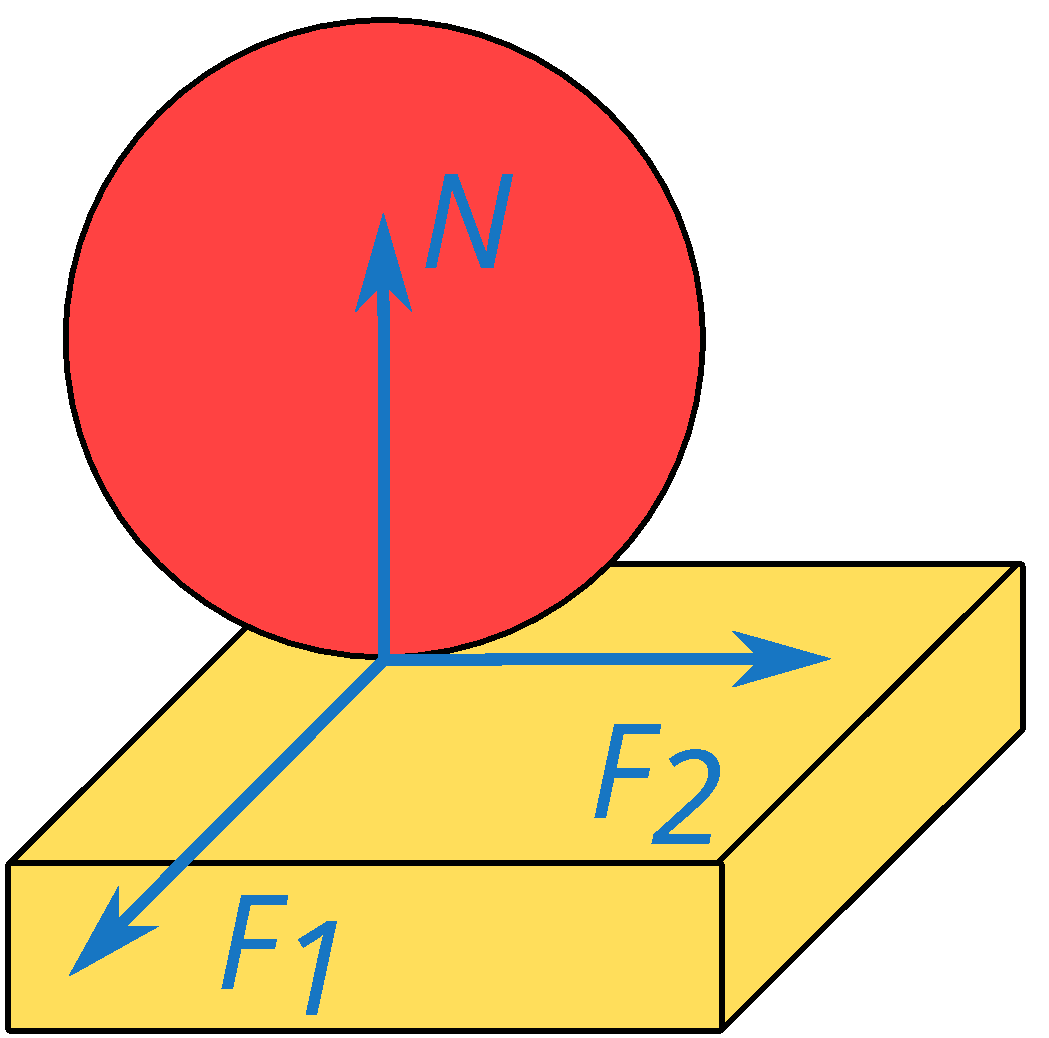
\includegraphics[width=0.5\textwidth]{graphics/friction.pdf}
		\caption{Wektory punktu kolizji.}
		\end{figure} 

		Po wykryciu punktu kolizji i wyznaczeniu wektora normalnych $N$ do dotykających się obiektów, system powinien zadziałać odpowiednimi siłami, 
		aby zatrzymać, lub odbić obiekty od siebie.
		Dodatkowo, ponieważ prędkości obiektów nie muszą być równoległe do wektora kolizji, należy zasymulować siłę tarcia z odpowiednią dla współczynnika tarcia wartością.
		Można to uzyskać, nadając obiektom w punkcie kolizji siłę prostopadłą do wektora normalnych, 
		ten wektor może być rozpisany przy pomocy dwóch wektorów jednostkowych $F_1$ i $F_2$. 
		Te wektory zawsze są prostopadłe do wektora normalnych, równoległe do płaszczyzny kolizji.

		W normalnej symulacji fizyki nigdy nie potrzeba osobno modyfikować współczynników tarcia i kierunku tych wektorów, 
		gdyż zazwyczaj powierzchnie symulowanych obiektów mają równe współczynniki tarcia w każdym kierunku.
		Jednakże modyfikując te wektory statycznie, lub dynamicznie, można uzyskać bardzo interesujące efekty.
		Instrukcja silnika symulacji podaje przykład, w którym aby zamodelować tarcie opon samochodu na zakręcie, prostopadle do kierunku jazdy, 
		należy dynamicznie zmieniać współczynnik tarcia dla wektora $F_1$, lub $F_2$ w kierunku promienia koła.
		Ten współczynnik tarcia, prostopadły do kierunku jazdy, może być liniowo zależny od prędkości.
		Spowoduje to, że im większa prędkość samochodu, tym boczna siła odśrodkowa bardziej wpłynie na tor jego jazdy, co ma odwzorowanie w rzeczywistości.
		Więcej informacji można znaleźć na stronie instrukcji maszyny symulacyjnej ODE \cite{ode_contact}.

		W opisywanym tutaj modelu, modyfikuje się wektor $F_1$, oraz współczynniki tarcia w obu kierunkach, aby przybliżyć zachowanie się rolki.
		Ponieważ wektory $F_1$ i $F_2$ są określone w lokalnym dla koła układzie współrzędnych, 
		w każdej iteracji maszyny symulacji należy obrócić je względem aktualnej pozycji bazy i odwrotności obrotu koła.
		Idealna rolka obraca się całkowicie bez tarcia, a ruch wzdłuż jej osi jest niemożliwy.
		Można więc ustawić zerowy współczynnik tarcia w kierunku prostopadłym do osi, oraz nieskończenie duży dla wektora równoległego do osi.

		\begin{figure}[H]
		\centering
		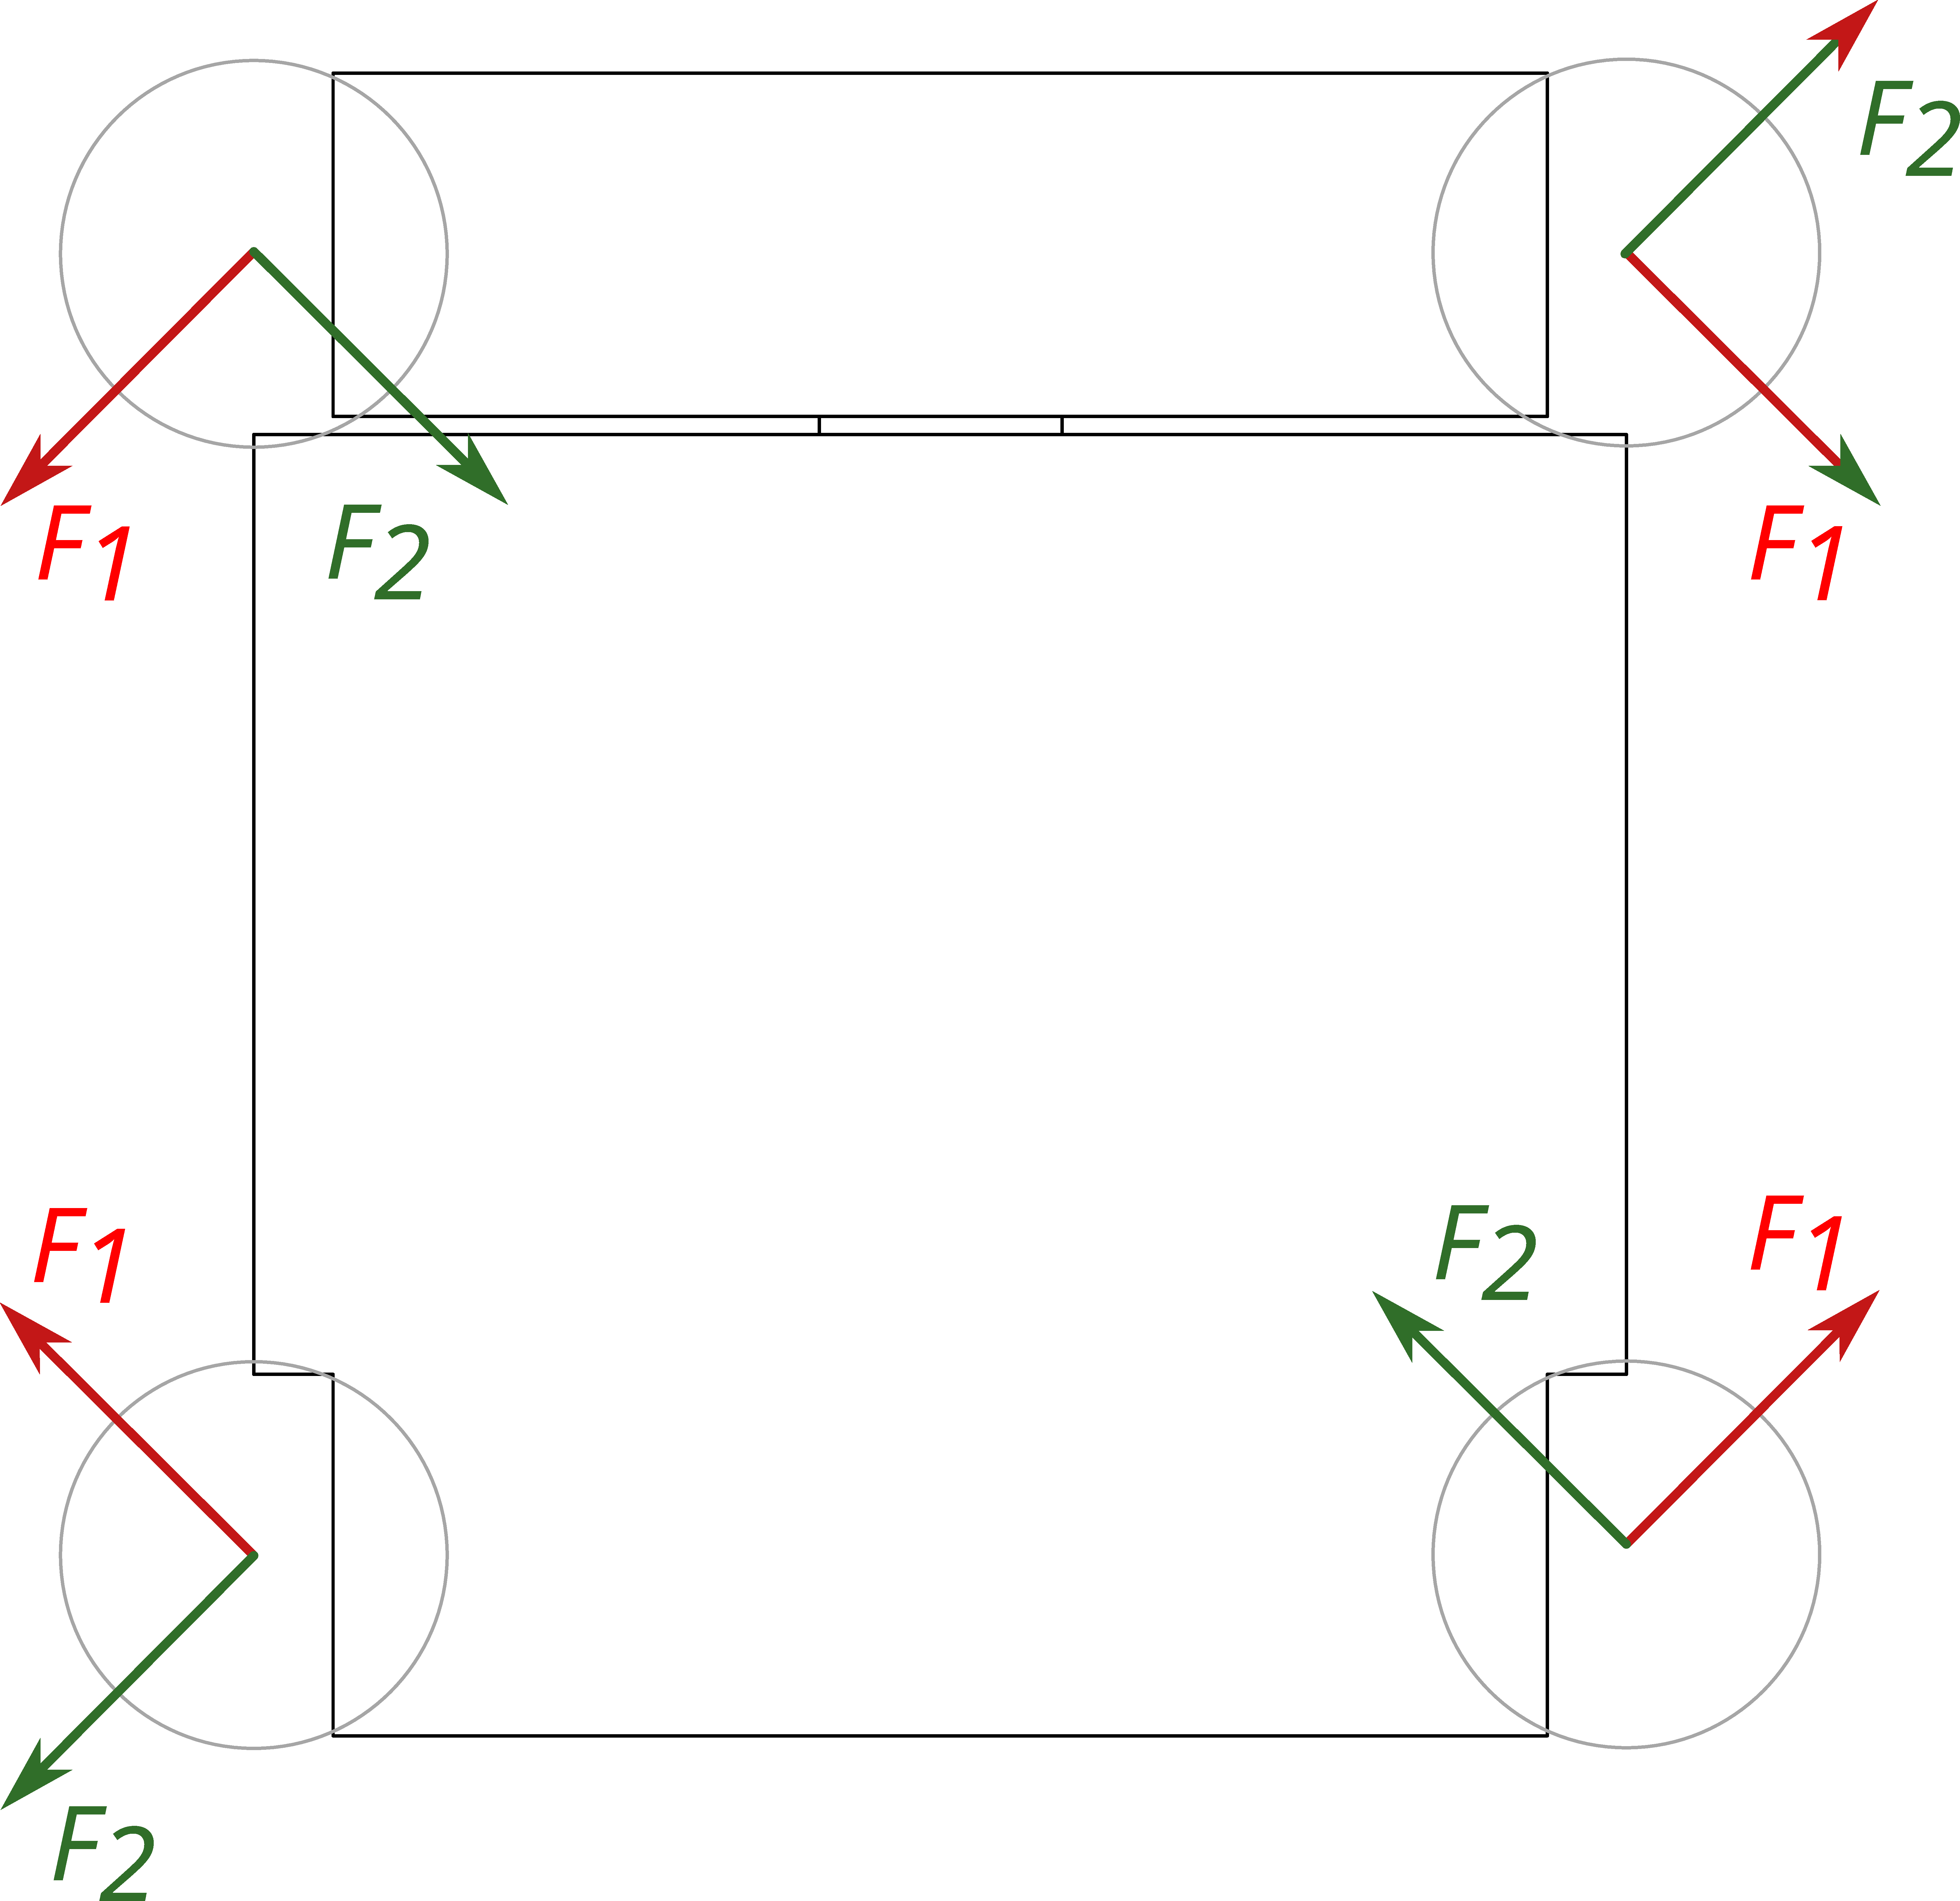
\includegraphics[width=0.8\textwidth]{graphics/base_vects.pdf}
		\caption{Kierunki wektorów dla których należy nadać współczynniki tarcia przy symulacji platformy, widok z góry. Tarcie w kierunku $F_1$ powinno być nieskończone, a w $F_2$ zerowe.}
		\end{figure} 

		Niestety, w rzeczywistości rolki wykonane są ze śliskiego plastiku, który zezwala na poślizg kół wzdłuż ich osi.
		Osie kolek również nie obracają się płynnie, trzeba użyć dużej siły, aby obrócić dowolną z nich, pod naciskiem platformy tarcie jest jeszcze większe.
		Każda rolka obraca się z innym tarciem wprowadzając kolejne zakłócenia.
		Podłoże po którym porusza się robot także nie jest tu bez znaczenia.
		Należy zatem wystawić interfejs do łatwej zmiany współczynników tarcia, aby później dobierać odpowiednie wartości na podstawie zachowania rzeczywistego robota.

		Podobnie, jak w poprzednich przypadkach, modeluje się tylko najniższą, dotykającą podłoża rolkę.
		Jak wcześniej wspomniano, ma ona bardzo skomplikowany kształt, lecz można przybliżyć całe koło kulą.
		Zatem w miejscu każdego koła zamontowana jest kula z dynamicznie modyfikowanym tarciem i siatką w kształcie koła do wizualizacji, 
		oraz przegub z motorem łączący odpowiednią część bazy z kołem.
		To najprostsza budowa modelu (a zatem najszybsza) z poprzednich.
		
		\begin{figure}[H]
		\dirtree{%
		.1 kadłub\DTcomment{Podstawa bazy}.
		.2 przegub z silnikiem\DTcomment{Nadaje moment obrotowy na żądanie}.
		.3 kula\DTcomment{Modyfikowane wektory tarcia}.
		.4 siatka\DTcomment{Odpowiada za wygląd obiektu koła}.
		}
		\caption{Zagnieżdżenie obiektów koła w strukturze drzewiastej z modyfikowanymi wektorami tarcia. W implementacji Gazebo przegub i kula są zagnieżdżone równolegle.}
		\label{fig:omnivelma_wheel}
		\end{figure}

		Takie rozwiązanie wiąże się z pewnym ryzykiem.
		Wymaga, aby symulator używał maszyny ODE, co zmniejsza przenośność modelu. ODE jest domyślnym symulatorem w Gazebo.
		Maszyna Bullet również liczy kolizje w ten sposób i ma modyfikowalne wektory, 
		lecz nie daje podobnych wyników. Być może jest to spowodowane brakiem odpowiedniej konfiguracji, lub innym wewnętrznym traktowaniem modelu.

	\subsection{Komunikacja}
		Ze względu na wiele ustawień elementów bazy, należy stworzyć bogaty interfejs.
		W każdym cyklu symulacji, program sterujący modelem platformy nadaje wiadomości:
		\begin{itemize}
		\item \texttt{geometry\_msgs/PoseStamped} z aktualną pozycją i rotacją platformy, oraz nagłówek z czasem i identyfikatorem.
		\item \texttt{geometry\_msgs/TwistStamped} z aktualną prędkością platformy i nagłówkiem.
		\item \texttt{omnivelma\_msgs/EncodersStamped} z odczytaną ze stanu obiektów kół aktualną rotacją i pozycją, z nagłówkiem. 
		To jest symulator enkoderów wbudowanych w silniki platformy.
		\end{itemize}
		
		Przyjmowane są także dane:
		\begin{itemize}
		\item \texttt{omnivelma\_msgs/Vels} z zadanymi prędkościami kół.
		\item Wywołanie ustawiające współczynniki tarcia wzdłuż wektorów $F_1$ i $F_2$.
		\item Wywołanie ustawiające masy i momenty obrotowe niektórych elementów składowych konstrukcji.
		\end{itemize}

	\subsection{Rozszerzenie modelu}
		\label{sec:model_nan}
		Ponieważ komputerowa reprezentacja liczby zmiennoprzecinkowej pozwala na zapisanie nie tylko liczbowych wartości, można rozszerzyć model o dodatkową funkcjonalność,
		wywoływaną wysłaniem do modelu cichej nie-liczby (\emph{NaN}) w wiadomości, w polu prędkości odpowiedniego koła. 
		Cicha nie-liczba powstaje w procesorze, w module operacji zmiennoprzecinkowych, przy przeprowadzaniu nieprawidłowych, 
		acz niekrytycznych obliczeń, na przykład dzielenie przez zero, lub dzielenie nieskończoności przez minus-nieskończoność 
		(także zapisywane jako forma liczby zmiennoprzecinkowej).
		Takie operacje nie powodują błędu programu, jedynie wynik w postaci nie-liczby propaguje przez wszystkie pozostałe operacje.

		Nadanie prędkości modelom w przestrzeni wirtualnej polega na wywołaniu odpowiedniej funkcji maszyny symulującej fizykę.
		Można zadać pytanie, jak zachowa się model, jeśli dla niektórych kół nie zmieniać prędkości po każdym odebraniu pakietu?

		Wobec tego, jeśli w pakiecie z nowymi prędkościami kół znajdzie się cicha nie-liczba, program sterujący nie nada nowej prędkości temu kołu.
		Jest to podobne do nadania tej samej prędkości, jaką posiada aktualnie obiekt koła (jaką zwróciłby enkoder).

		Zwraca to uwagę również na potrzebę, aby program do komunikacji z rzeczywistym robotem nie skończył się błędem po odebraniu jednej z takich nieokreślonych wiadomości.
		Ponieważ przekształca liczby zmiennoprzecinkowe, zawarte w ROSoswych pakietach, na dane zrozumiałe przez sterownik silnika, które zazwyczaj są liczbami
		stałoprzecinkowymi, program może zachować się nieprzewidywalnie.
 
\chapter{Implementacja} 
\label{sec:implementation}
W tym rozdziale opisane są szczegóły techniczne zastosowanych rozwiązań.

\section{Istniejące implementacje}
	Istnieją także inne modele jeżdżących robotów na kołach szwedzkich.
	Można z nich brać przykład i sugerować się źródłami kodu i budową modeli.

	Kuka Youbot jest popularnym robotem wielokierunkowym. Jego modele są domyślnie dostępne w różnych symulatorach, między innymi w Gazebo i V-Repie, które są dobrymi kandydatami do 
	użycia w projekcie.
	Tylko w przypadku V-Repa, istnieje wstępny sterownik do którego da się wysyłać odpowiednie wartości kierunku, a on nadaje takie prędkości kołom, aby poruszać modelem w zadanym kierunku.
	Wersja dla Gazebo jest statycznym obiektem z błędnie ustanowionymi przegubami, jego efektory nie są zaimplementowane.
	
	Dodatkowo, V-Rep posiada wbudowane dwa inne pojazdy o napędach kół Mecanum i czujnikach laserowych.
	Zewnętrzne modele także pomogą przy wstępnej weryfikacji zachowania się budowanego tutaj modelu, czy nie zachowuje się nadzwyczaj dziwnie w pierwszych fazach projektu.

	Ze względu na niezwykle zaawansowany obiekt kół i kształt rolek, ważne jest aby uprościć model, poprzez zamianę niektórych składowych i dodanie sztucznych więzów.
	Całościowy model może być zbyt skomplikowany, aby maszyny symulacji mogły go obliczać w czasie rzeczywistym.
	Dokładny model także jest znacznie trudniej poprawnie wymodelować, ze względu na liczne tarcia i poślizgi rolek.
	Proponowane uproszczenia modeli opisane są w sekcji \ref{sec:omnivelma}.
	

\section{Ogólne typy implementacji}
	\subsection{Program wykonywalny w ROS}

	\subsection{Wtyczka Gazebo}
		\subsubsection{Wtyczka sterownika modelu}
		\subsubsection{Wtyczka sterownika czujnika}
	
\section{Program ręcznego sterowania}
%TODO diagram klas


%TODO implementacja wszystkiego

\chapter{Testy systemu}
W tym rozdziale przedstawione są różne konfiguracje pakietów, wraz z wykresami ruchów platform, oraz wnioski płynące z tych zachowań.

% \section{Porównanie modeli dynamiki i kinematyki}
% 	Posiadając model kinematyczny, którego ruch jest sterowany wzorami, można porównać jego pozycję i rotację z modelem dynamicznym.
% 	Należy w tym samym momencie nadać bazom identyczne prędkości kół i zebrać dane dotyczące wzajemnej pozycji.
% 	Nadano kołom kolejne prędkości zgodnie z numeracją w rysunku \ref{fig:base_dims}, $[-2 , 1 , 0 , -3]$.
% 	Do zebrania pomiarów posłużył pakiet \texttt{ocznica}.
% 
% 	\begin{figure}[H]
% 	\centering
% 	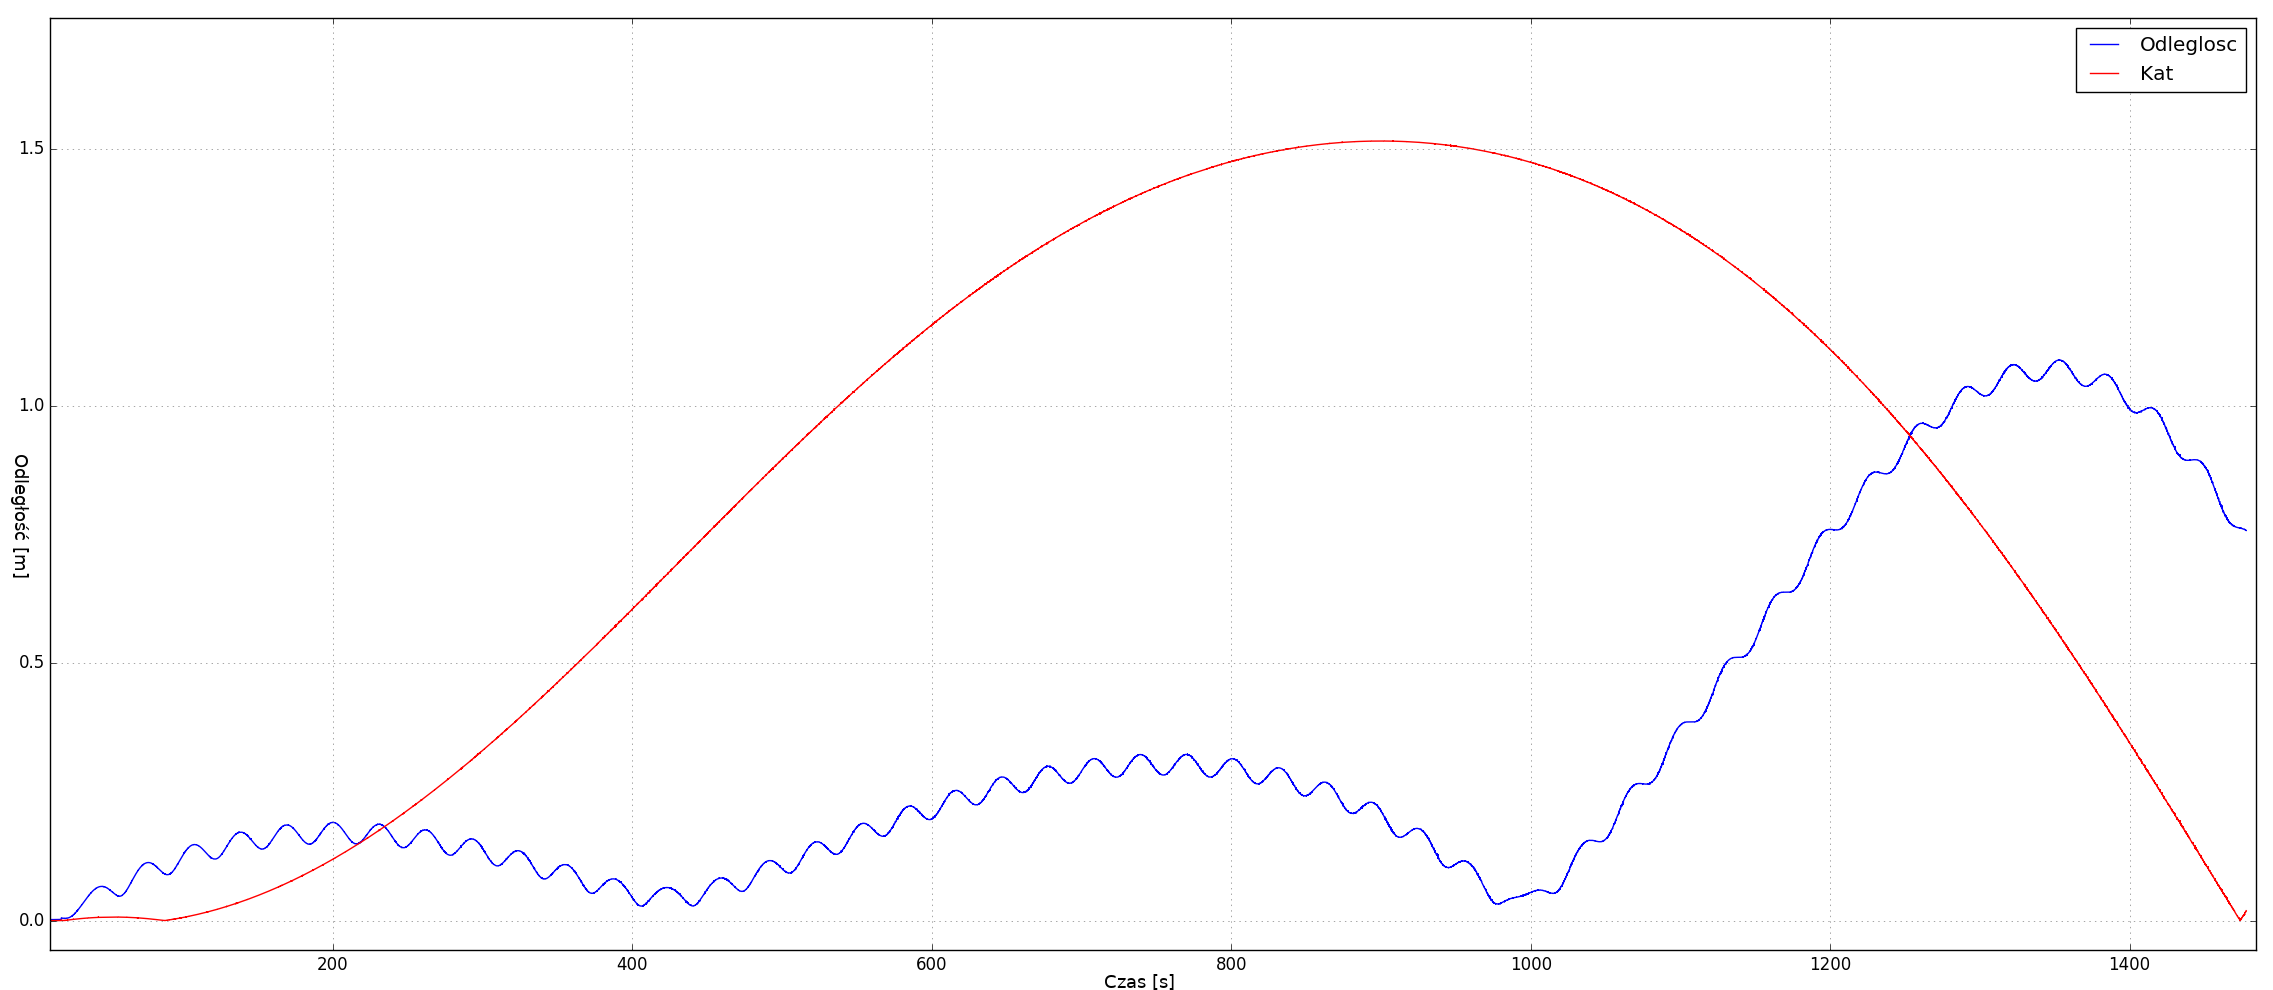
\includegraphics[width=\textwidth]{graphics/test1.png}
% 	\caption{Odległość i kąt pomiędzy platformami w czasie.}
% 	\end{figure} 
% 
% 	%TODO połączenie komponentów na UML, jak nie Tikz to Draw.io
% 	
% 	Takie ustawienie spowodowało ruch po okręgu o okresie ok. 32 s.
% 	Modele początkowo posiadały zbliżoną pozycję i rotację, ale w miarę upływu czasu opóźnienia modelu dynamicznego stały się zauważalne.
% 	Także kąt między nimi zaczął się zmieniać, lecz w znacznie większym stopniu, niż wynikałoby to z opóźnienia pozycji.
% 	Przez cały czas trwania eksperymentu model dynamiczny zrobił kąt pełny w stosunku do kinematycznego, a jego odległość zmieniała się sinusoidalnie.
% 	Oba modele wykonały taką samą ilość obiegów.
% 
% 	Po pierwsze widać, że już na samym początku pomiarów odległość nagle wzrosła, co jest spowodowane poślizgiem platformy przy nadaniu kołom prędkości.
% 	Model kinematyczny rozpoczyna jazdę natychmiastowo.
% 	Dzieje się tak, pomimo doskonałym współczynnikom tarcia, w dodatku masa platformy nie jest dobrana zgodnie z rzeczywistością, a lżejsza.
% 	Ten efekt może być zmniejszony za pomocą ustawiania współczynnika tarcia podłoża, ale nie jest możliwe jego całkowite wyeliminowanie, gdyż jest to cecha maszyn symulacji fizyki.
% 
% 	Drugą zauważalną cechą wykresu są małe oscylacje o okresie jednego obiegu.
% 	Ma to efekt taki sam, jak gdyby obie platformy wystartowały z różnych pozycji, których odległość jest mniejsza od średnicy trasy.
% 	To powodowałby, że odległość między ich pozycjami oscylowałaby w właśnie taki sposób.
% 	Modele wystartowały z tego samego punktu w tym samym czasie, jednakże środek ciężkości modelu dynamicznego nie pokrywał się ze środkiem platformy względem którego obliczano pozycję.
% 	W związku z tym jej ruch odbywa się wokół środka ciężkości masy, ale pozycja jest liczona względem geometrycznego środka.
% 	To pokazuje, że należy bardzo dokładnie ustawić masy elementów składowych w stosunku do rzeczywistego modelu, gdyż w przeciwnym wypadku symulacja obarczona będzie właśnie takimi oscylacjami.
% 	Co więcej, ruchome elementy transportowanego robota manipulującego będą miały wpływ na pozycję środka ciężkości i ruch podstawy.
% 	Dlatego należy wprowadzić element transportowanej masy, którego środek ciężkości powinien być modyfikowalny.
% 
% 	Trzecią cechą są duże oscylacje, rosnące w czasie.
% 	Na razie nie jest dokładnie wiadome, dlaczego powstają.
% 	Warto jednak zauważyć, że nie są zbieżne w czasie z kątem obrotu, gdyż jego wartość ma mniejszy okres.
% 
% 	Opóźnienia powstałe na modelu dynamicznym są cechą dokładności maszyny symulacyjnej fizyki i nie da się ich całkowicie wyeliminować.
% 	Jednakże ich wartość jest znacznie mniejsza od niedokładności wprowadzonej przez niedoskonałość rzeczywistego obiektu.
% 	To oznacza, że model ma rzeczywistą wartość pod kątem pomocy w symulacji robota.



\chapter{Podsumowanie}
\label{sec:ending}

Stworzono modele platform oraz czujników, a także system wielu innych pakietów usprawniających testowanie i sterowanie robotem.

Eksperymenty przeprowadzone na modelu i platformie pokazały, że błędy lokalizacji w modelu mogą być nawet większe, niż w rzeczywistym robocie.
Z punktu widzenia testowania programu symulacyjnego jest to przydatne, gdyż program sterujący, przetestowany na symulatorze, na pewno poprawnie określi sterowanie
dla robota o mniejszych błędach ruchu.
Model kinematyki posiada bardzo wiele parametrów działania, nie tylko w kwestii mas ogniw i ich momentów bezwładności, ale
także w kwestii obsługi maszyny symulacyjnej fizyki.
Istnieje kilka sposobów na nadawanie prędkości kątowej kołom.
Aby znaleźć najodpowiedniejszy, należy przeprowadzić czasochłonne badania nad działaniem każdego z nich, również biorąc pod uwagę sposób działania maszyny do symulacji.
Sama maszyna może być modyfikowana w celu lepszego zamodelowania bazy (gdyż ma otwarty kod), lub zastąpiona inną maszyną do symulacji fizyki.

Testy pokazały również, jak wiele różnych i czasami nielogicznych zachowań występuje w modelach i robocie.
Sama poprawna interpretacja wszystkich tych cech wykresów wymaga dogłębnego zbadania działania robota i maszyny do symulacji fizyki.

Ponieważ model posiada uproszczone modele kół Mecanum, niektóre ich cechy (jak na przykład opór obrotowy rolek) nie mogą być zamodelowane
lub też istnieje jakiś nietypowy sposób (na przykład nieznaczna zmiana kierunku wektora siły tarcia) na zamodelowanie takich własności.

Jednostka inercyjna wykrywa własności robota, nieistniejące w modelu, na przykład drgania powstałe przy nagłej zmianie prędkości platformy.
Próby wprowadzania takich własności do modelu mogą nie być możliwe lub też wymagać kolejnych badań, na przykład w kwestii dodania sprężystości do niektórych więzów.
Istnieje także minimalny szum, zależny w dużym stopniu od ustawień parametrów modelu.

Model skanera laserowego jest bardzo prosty w działaniu, zatem jego ewentualny rozwój nie będzie aż tak skomplikowany, jak innych czujników.

Pakiety pomocnicze i skrypty uruchamiające okazały się przydatne w sterowaniu platformą, jednak niektóre były nadto skomplikowane i niepotrzebne.
Pakiet rozdzielania sterowania platformy może być zastąpiony przez kilkukrotne wywołanie wbudowanego pakietu.
Program do ręcznego sterowania jest nadto skomplikowany a i tak nie był używany do sterowania robotem, ani do przeprowadzania testów z rozdziału \ref{sec:tests}.
Stanowią jednak one dobre wspomaganie do późniejszego rozwijania modelu w celu odpowiedniego ustawienia parametrów, aby jak najdokładniej przybliżyć jej działanie do platformy.



\begin{thebibliography}{0}

% stosowanie_modelu.pdf
\bibitem{kinematic_modeling}
P. Muir, C. Neuman,
``Kinematic modeling for feedback control of an omnidirectional wheeled mobile robot'', 
Proceedings, IEEE International Conference in Robotics and Automation, 
Vol 4. pp. 1772-1778, 1987.

% koła.pdf
\bibitem{wheels}
M. O. Tătar, C. Popovici, D. Mândru, I. Ardelean, A. Pleşa,
``Design and development of an autonomous omni-directional mobile robot with Mecanum wheels'',
Conference: 2014 IEEE International Conference on Automation, Quality and Testing, Robotics,
Cluj-Napoca, 2014, pp. 1-6. DOI: 10.1109/AQTR.2014.6857869.

% paletobot.pdf
\bibitem{paletobot}
M. Lamy, 
``Mechanical development of an automated guided vehicle'',
Master of Science Thesis MMK 2016:153 MKN 171,
KTH Industrial Engineering and Management,
Machine Design.

% matematyka_rolki.pdf
\bibitem{rollers}
A. Gfrerrer, 
``Geometry and kinematics of the Mecanum wheel'',
Computer Aided Geometric Design,
25(9):784-791.

% silny_robot.pdf
\bibitem{heavy}
L. Xie, C. Scheifele, W. Xu, K. A. Stol, 
``Heavy-Duty Omni-Directional Mecanum-Wheeled Robot for Autonomous Navigation'',
2015 IEEE International Conference on Mechatronics (ICM), Nagoya, 2015, pp. 256-261.
DOI: 10.1109/ICMECH.2015.7083984.

% hamowanie.pdf
\bibitem{braking}
V. Kálmán, 
``On modeling and control of omnidirectional wheels'',
PhD. dissertation, Budapest University of Technology and Economics,
Department of Control Engineering and Information Technology,
Budapeszt 2013.

% ruchome_osie.pdf
\bibitem{extra_axis}
J.B. Song, K.S. Byun,
``Design and Control of a Four-Wheeled Omnidirectional Mobile Robot with Steerable Omnidirectional Wheels'',
Journal of Robotic Systems,
21(4):193-208, 
Kwiecień 2004.

% jakiśtam.pdf
\bibitem{boringbot}
I. Doroftei, V. Grosu, V. Spinu,
``Omnidirectional Mobile Robot – Design and Implementation'',
Bioinspiration and Robotics Walking and Climbing Robots, M. K. Habib (Ed.), 
ISBN: 978-3-902613-15-8, InTech,
2007.

% sposoby_modelowania.pdf
\bibitem{modelling_ways}
V. Kálmán,
``Omnidirectional Wheel Simulation --- a Practical Approach'',
Acta Technica Jaurinensis,
6(2):73-90,
2013.

\bibitem{gazebo_website}
Strona internetowa symulatora Gazebo. \\
\url{http://gazebosim.org}

\bibitem{vrep_website}
Strona internetowa symulatora V-Rep. \\
\url{http://coppeliarobotics.com}

\bibitem{ros_website}
Strona internetowa programowej struktury ramowej \emph{Robot Operating System}. \\
\url{http://www.ros.org}

\bibitem{sdf_website}
Strona internetowa standardu SDF. \\
\url{http://sdformat.org/spec}

\bibitem{sick_website}
Strona internetowa SICK, producenta czujników laserowych. \\
\url{https://www.sick.com/de/en/detection-and-ranging-solutions/2d-lidar-sensors/lms1xx/lms100-10000/p/p109841}

\bibitem{adis_website}
Strona internetowa sprzedawcy czujnika inercji. \\
\url{https://www.digikey.com/product-detail/en/analog-devices-inc/ADIS16460AMLZ/ADIS16460AMLZ-ND/5957823}

\bibitem{ode_contact}
Dokumentacja ODE z wyjaśnieniem działania kolizji. \\
\url{http://ode-wiki.org/wiki/index.php?title=Manual:_Joint_Types_and_Functions#Contact}

\bibitem{andymark}
Strona internetowa producenta kół Mecanum, użytych w platformie. \\
\url{http://www.andymark.com/8in-Mecanum-HD-Set-p/am-2118.htm}

\end{thebibliography}


\end{document} 
